% گزارش KG-GT v2. کامپایل: xelatex main.tex (دو بار، برای فهرست و ارجاع‌ها)
\documentclass[11pt,a4paper]{article}
\usepackage[margin=2.2cm]{geometry}
\usepackage{amsmath,amssymb,bm}
\usepackage{graphicx,booktabs,float,array}
\usepackage{placeins}
\usepackage{tikz}
\usetikzlibrary{positioning,arrows.meta,fit,calc,shapes.geometric,backgrounds,decorations.pathreplacing}
\usepackage[colorlinks=true,linkcolor=black,citecolor=black,urlcolor=black]{hyperref}
\usepackage{xepersian}
\settextfont[Path=fonts/,BoldFont=Vazirmatn-Bold.ttf,ItalicFont=Vazirmatn-Medium.ttf,BoldItalicFont=Vazirmatn-Bold.ttf]{Vazirmatn-Regular.ttf}
\setlatintextfont[Path=fonts/,BoldFont=Vazirmatn-Bold.ttf,ItalicFont=Vazirmatn-Medium.ttf,BoldItalicFont=Vazirmatn-Bold.ttf]{Vazirmatn-Regular.ttf}
\setdigitfont[Path=fonts/,BoldFont=Vazirmatn-Bold.ttf,ItalicFont=Vazirmatn-Medium.ttf,BoldItalicFont=Vazirmatn-Bold.ttf]{Vazirmatn-Regular.ttf}

\linespread{1.25}
\setlength{\parskip}{0.35em}
\renewcommand{\arraystretch}{1.12}
\setcounter{tocdepth}{2}

% سبک‌های نمودار: متن همه‌ی نمودارها انگلیسی و چپ‌به‌راست است (فقط زیرنویس‌ها فارسی‌اند).
\definecolor{kinc}{HTML}{EB6834}\definecolor{eegc}{HTML}{2A78D6}\definecolor{fusc}{HTML}{1BAF7A}\definecolor{intc}{HTML}{7B4FB5}
\tikzset{
  box/.style={draw, rounded corners=2pt, align=center, minimum height=7mm, inner sep=3pt, font=\footnotesize, fill=white,
              execute at begin node={\hyphenpenalty=10000\exhyphenpenalty=10000}},
  io/.style={box, fill=black!6},
  result/.style={box, line width=0.9pt},
  kbox/.style={box, fill=kinc!10, draw=kinc!70!black},
  ebox/.style={box, fill=eegc!10, draw=eegc!70!black},
  fbox/.style={box, fill=fusc!12, draw=fusc!70!black},
  arr/.style={-{Stealth[length=2mm]}, semithick},
  darr/.style={arr, dashed},
  grp/.style={draw, dashed, rounded corners=3pt, inner sep=6pt},
  lab/.style={font=\scriptsize, align=center},
  mnode/.style={circle, draw, minimum size=6.2mm, inner sep=0pt, font=\tiny\bfseries, fill=white},
  enode/.style={circle, fill=eegc!80!black, minimum size=1.6mm, inner sep=0pt},
}
% ---- رسم‌های تکرارشونده: گراف پنج عضله، سر با الکترودها، بلوک ترنسفورمر، سیگنال
% \musclegraph{prefix}{center}{radius}{color}
\newcommand{\musclegraph}[4]{%
  \foreach \m/\a in {AD/90,BR/18,FD/-54,ED/-126,FDI/162}{\node[mnode, draw=#4!70!black, fill=#4!8] (#1\m) at ($(#2)+(\a:#3)$) {\m};}
  \foreach \u/\v in {AD/BR,AD/FD,AD/ED,AD/FDI,BR/FD,BR/ED,BR/FDI,FD/ED,FD/FDI,ED/FDI}{\draw[#4!45, line width=0.5pt] (#1\u)--(#1\v);}
  \draw[-{Stealth[length=1.4mm]}, #4!80!black, line width=0.9pt] (#1FD)--(#1AD);
  \draw[-{Stealth[length=1.4mm]}, #4!80!black, line width=0.9pt] (#1ED)--(#1BR);}
% \headgraph{prefix}{center}{radius}
\newcommand{\headgraph}[3]{%
  \draw[black!60] (#2) circle (#3);
  \draw[black!60] ($(#2)+(-0.13*#3,0.99*#3)$)--($(#2)+(0,1.17*#3)$)--($(#2)+(0.13*#3,0.99*#3)$);
  \foreach \x/\y [count=\i] in {-0.3/0.75,0.3/0.75,-0.6/0.4,-0.2/0.4,0.2/0.4,0.6/0.4,-0.75/0,-0.35/0,0/0,0.35/0,0.75/0,-0.6/-0.4,-0.2/-0.4,0.2/-0.4,0.6/-0.4,-0.3/-0.75,0.3/-0.75}{\node[enode] (#1\i) at ($(#2)+(\x*#3,\y*#3)$) {};}
  \foreach \u/\v in {8/9,9/10,3/8,4/9,5/9,9/13,9/14,8/12,10/15,4/5,2/6}{\draw[eegc!60, line width=0.4pt] (#1\u)--(#1\v);}}
% \tblock{name}{position}{width}{title}{N}{color}: بلوک ترنسفورمر با نرمال‌سازی پیشین
% The title sits inside the block, so arrows reach its border without crossing text.
% \tblock{name}{position}{width}{title}{N}{color}{line above attention}{line above FFN}{bottom note}
\newcommand{\tblock}[9]{%
  \node[draw=#6!70!black, fill=#6!6, rounded corners=3pt, minimum width=#3, minimum height=3.1cm] (#1) at (#2) {};
  \node[lab, font=\scriptsize\bfseries] at ($(#1)+(0,1.25)$) {#4};
  \node[lab, font=\tiny, text=black!70] at ($(#1)+(0,0.84)$) {#7};
  \node[box, minimum width=#3-5mm, minimum height=5mm, font=\scriptsize] (#1a) at ($(#1)+(0,0.4)$) {Multi-head attention};
  \node[lab, font=\tiny, text=black!70] at ($(#1)+(0,-0.12)$) {#8};
  \node[box, minimum width=#3-5mm, minimum height=5mm, font=\scriptsize] (#1f) at ($(#1)+(0,-0.56)$) {Feed-forward};
  \node[lab, font=\tiny, text=black!70] at ($(#1)+(0,-1.18)$) {#9};
  \node[lab, font=\bfseries\small, anchor=west] at (#1.east) {$\times$#5};}
% attnmap{name}{center}{n}{cell}{shift}{color}{diagonal boost}: a small attention-like heat map, rows = queries
\newcommand{\attnmap}[7]{%
  \begin{scope}[shift={(#2)}]
  \foreach \i in {1,...,#3}{\foreach \j in {1,...,#3}{%
    \pgfmathsetmacro\hmv{min(92,10+58*exp(-abs(\j-\i+#5)/1.5)+#7*(\i==\j))}%
    \fill[#6!\hmv] ({(\j-1-#3/2)*#4},{(#3/2-\i)*#4}) rectangle ++(#4,#4);}}
  \draw[black!55] ({-#3/2*#4},{-#3/2*#4}) rectangle ({#3/2*#4},{#3/2*#4});
  \coordinate (#1) at (0,0);
  \coordinate (#1-n) at (0,{#3/2*#4}); \coordinate (#1-s) at (0,{-#3/2*#4});
  \coordinate (#1-w) at ({-#3/2*#4},0); \coordinate (#1-e) at ({#3/2*#4},0);
  \end{scope}}
% \sig{start}{length}{amplitude}{color}{seed-phase}: یک سیگنال کوچک
\newcommand{\sig}[5]{\draw[#4, line width=0.6pt, domain=0:#2, samples=60, smooth] plot (\x+#1, {#3*(0.55*sin(\x*190+#5)+0.35*sin(\x*530+2*#5)+0.2*sin(\x*1100+3*#5))});}
\newcommand{\env}[5]{\draw[#4, line width=0.8pt, domain=0:#2, samples=60, smooth] plot (\x+#1, {#3*max(0, sin(\x*120+#5))^2});}

\newcommand{\fig}[3]{\begin{figure}[htbp]\centering\includegraphics[width=#2\textwidth,height=0.8\textheight,keepaspectratio]{figures/#1}\caption{#3}\label{fig:#1}\end{figure}}

\title{گزارش مدل \lr{KG-GT v2}:\\ پیش‌بینی پوش \lr{EMG} از سینماتیک و \lr{EEG} با تفسیرپذیری در همه‌ی لایه‌ها}
\author{تیم ۶، مدرسه‌ی بین‌رشته‌ای علوم اعصاب محاسباتی}
\date{مهر ۱۴۰۵}

\begin{document}
\maketitle

\begin{abstract}
این گزارش دو مدل را مقایسه می‌کند که فعالیت پنج عضله‌ی دست و بازو (پوش \lr{EMG}) را در داده‌ی \lr{WAY-EEG-GAL} پیش‌بینی می‌کنند. در این داده ۱۲ نفر بارها جسمی را گرفته و بلند کرده‌اند.

مدل پایه (\lr{KG-GT}، دفترچه‌ی \lr{main\_1stage} در شاخه‌ی \lr{KG-GT-CUDA}) یک \lr{Transformer} روی \lr{EEG} و یک \lr{muscle graph} دارد که سینماتیک دست آن را هدایت می‌کند، و فقط یک خروجی می‌دهد. روی سری‌های آزمون به \lr{VAF} \lr{۷۲٫۲} درصد و همبستگی \lr{۰٫۸۵۱} رسید. اما آزمون‌های حذف ورودی نشان دادند تقریباً همه‌ی این دقت از سینماتیک می‌آید، و با یک خروجی نمی‌توان سهم \lr{EEG} را جدا کرد.

مدل \lr{v2} سه خروجی جدا دارد: \lr{K} فقط از سینماتیک و تاریخچه‌ی بلندکردن‌ها، \lr{E} فقط از \lr{EEG}، و \lr{F} که \lr{K} را با یک اصلاح کوچک از \lr{EEG} جمع می‌کند. \lr{K} با \lr{VAF} \lr{۷۵٫۸} درصد و $r$ \lr{۰٫۸۷۲} در هر ۱۲ نفر از مدل پایه بهتر شد. \lr{E} به‌تنهایی به $r$ \lr{۰٫۶۴۵} رسید و در هر ۱۲ نفر از \lr{null test} گذشت. \lr{F} عملاً با \lr{K} برابر ماند. \lr{residual test} نشان داد \lr{EEG} فقط اطلاعات بسیار کمی درباره‌ی خطای \lr{K} دارد ($r$ حدود \lr{۰٫۰۷}، معنادار در ۱۰ نفر از ۱۲) که کمتر از نیم واحد به \lr{VAF} اضافه می‌کند.

\lr{v2} طوری ساخته شد که بتوان هر خروجی را از طریق همه‌ی لایه‌ها تا ورودی دنبال کرد: با \lr{attention rollout}، \lr{attention flow}، \lr{gradient-weighted rollout} و \lr{gradient × input}. خود این روش‌ها با \lr{deletion check} و \lr{weight-shuffle check} سنجیده شدند، یکسانی نقشه‌ها بین ۱۲ نفر اندازه گرفته شد و نتایج با پژوهش‌های پیشین مقایسه شد. نقشه‌ی گروهی \lr{EEG} کانونی تکرارپذیر روی \lr{C3} و \lr{CP1} دارد و باند بتا را ترجیح می‌دهد.
\end{abstract}

\tableofcontents
\newpage

\section{داده و هدف پیش‌بینی}

داده‌ی \lr{WAY-EEG-GAL} \cite{luciw2014} ثبت هم‌زمان \lr{EEG}، الکترومیوگرافی (\lr{EMG})، سینماتیک دست و نیروهای جسم را در آزمایش «گرفتن و بلندکردن» دارد. ۱۲ شرکت‌کننده جسمی را با دست راست می‌گیرند، بلند می‌کنند، چند ثانیه نگه می‌دارند و سر جایش می‌گذارند. وزن جسم (سبک، متوسط، سنگین) و جنس سطح تماس آن بین سری‌ها و گاهی بین بلندکردن‌ها تغییر می‌کند. هر سری چند ده بلندکردن پشت سر هم است.

هدف در هر دو مدل این گزارش، پوش \lr{EMG} پنج عضله است: دلتوئید قدامی (\lr{AD})، براکیورادیالیس (\lr{BR})، فلکسور انگشتان (\lr{FD})، اکستنسور انگشتان (\lr{ED}) و اولین بین‌استخوانی پشتی (\lr{FDI}). پوش با این مراحل ساخته می‌شود: فیلتر \lr{band-pass} ۳۰ تا ۳۰۰ هرتز روی سیگنال خام ۴۰۰۰ هرتز، عملگر انرژی \lr{TKEO}، \lr{low-pass} علّی ۸ هرتز و کاهش نرخ به ۵۰۰ هرتز. \lr{EMG} فقط هدف است و هیچ‌جا ورودی مدل نیست.

سری‌های هر شرکت‌کننده به سه دسته‌ی آموزش، \lr{validation} و آزمون تقسیم می‌شوند؛ تقسیم برای هر شرکت‌کننده جداگانه و لایه‌بندی‌شده بر اساس شرایط سری است و هر دو مدل از همین تقسیم استفاده می‌کنند. همه‌ی اعداد این گزارش روی سری‌های آزمون است (برای هر شرکت‌کننده دو سری).

معیارها برای هر عضله جدا حساب می‌شوند. اگر $y$ هدف و $\hat y$ پیش‌بینی باشد:
\begin{equation}
\mathrm{VAF}=100\left(1-\frac{\operatorname{Var}(y-\hat y)}{\operatorname{Var}(y)}\right),\qquad
\mathrm{CCC}=\frac{2\,\operatorname{Cov}(y,\hat y)}{\operatorname{Var}(y)+\operatorname{Var}(\hat y)+(\bar y-\bar{\hat y})^2},
\end{equation}
و $r$ \lr{Pearson correlation} است. \lr{VAF} هم شکل و هم دامنه را می‌سنجد و \lr{r} فقط شکل را. «\lr{height ratio}» میانگین پیش‌بینی به میانگین هدف در مرحله‌ی نگه‌داشتن جسم است و مقدار مطلوبش ۱ است.

\section{مدل پایه: \lr{KG-GT} در شاخه‌ی \lr{KG-GT-CUDA}}
\label{sec:base}

مدل پایه همان مدلی است که دفترچه‌ی \lr{main\_1stage.ipynb} در شاخه‌ی \lr{KG-GT-CUDA} آموزش می‌دهد. نام آن از «\lr{Transformer} گراف با هدایت سینماتیک» (\lr{Kinematics-Guided Graph Transformer}) آمده است. کل مدل در یک مرحله و یک‌جا آموزش می‌بیند.

\subsection{ورودی‌ها و خروجی}

\textbf{\lr{EEG}:} ۳۲ کانال با نرخ ۵۰۰ هرتز، پس از فیلتر \lr{band-pass} \lr{۰٫۵} تا ۴۰ هرتز، فیلتر ناچ ۵۰ هرتز و حذف خودکار \lr{artifact} با \lr{ICA}. سیگنال در حوزه‌ی زمان (نه \lr{band power}) به مدل داده می‌شود.

\textbf{سینماتیک:} ۲۴ ویژگی با نرخ ۵۰۰ هرتز: ۱۰ ویژگی وضعیت دست، نیروی بار ($F_L$) و نیروی گرفتن ($F_G$) که در یک «\lr{gate} نزدیکی دست به جسم» ضرب شده‌اند، ۱۰ سرعت وضعیت دست و سرعت دو نیروی \lr{gated}. \lr{gate} وقتی انگشت اشاره تا ۱۲ سانتی‌متری جسم است ۱ است و تا ۲۰ سانتی‌متر به‌تدریج به صفر می‌رسد؛ با آن، نیرویی که دیگران هنگام آماده‌سازی جسم وارد می‌کنند وارد مدل نمی‌شود. سرعت‌ها با فیلتر ساویتزکی‌گولای (پنجره‌ی ۵۱ نمونه) حساب می‌شوند و همه‌ی ویژگی‌ها با آماره‌های سری‌های آموزش استاندارد می‌شوند.

\textbf{پنجره:} یک ثانیه (۵۰۰ نمونه) بدون هم‌پوشانی. هدف در هر پنجره پوش \lr{EMG} استانداردشده (\lr{z-score}) است و خروجی مدل در پایان به واحد اصلی برمی‌گردد.

\subsection{معماری}

شکل~\ref{fig:base-arch} مسیر داده را نشان می‌دهد. با نماد $X^{e}\in\mathbb{R}^{T\times 32}$ برای \lr{EEG} و $X^{k}\in\mathbb{R}^{T\times 24}$ برای سینماتیک ($T=500$):

\begin{enumerate}
\item \textbf{\lr{temporal encoder}:} \lr{Transformer} با ۴ لایه، ۸ سر، عرض $d=128$ و شبکه‌ی \lr{feed-forward} ۵۱۲، با توجهِ تکه‌تکه (تکه‌های ۵۰۰ نمونه‌ای) و \lr{sinusoidal positional encoding}: $H=\mathrm{Enc}(X^{e})\in\mathbb{R}^{T\times128}$.
\item \textbf{تصویر به گره‌های عضله:} یک لایه‌ی خطی $H$ را به پنج گره با عرض ۶۴ می‌برد: $N_t\in\mathbb{R}^{5\times 64}$.
\item \textbf{\lr{muscle graph} با هدایت سینماتیک:} \lr{graph attention} (\lr{GAT} \cite{velickovic2018}) با ۴ سر بین پنج گره. امتیاز یال $j\to i$ در سر $h$ و زمان $t$ سه جزء دارد:
\begin{equation}
s^{h}_{ij}(t)=\frac{q^{h}_i(t)\cdot k^{h}_j(t)}{\sqrt{d_k}}+B^{h}_{ij}+\big[W x^{g}(t)+b\big]^{h}_{ij},
\end{equation}
که $B$ \lr{bias} ایستای یال‌هاست (مقداردهی اولیه از همبستگی \lr{EMG} آموزش) و $x^{g}(t)$ دوازده ویژگی اول سینماتیک (وضعیت دست و دو نیروی \lr{gated}) است که با یک لایه‌ی خطی به \lr{bias} پویای یال‌ها تبدیل می‌شود.
\item \textbf{\lr{kinematic skip highway}:} ۱۴ ویژگی (دو نیروی \lr{gated} و ۱۲ سرعت) از یک شبکه‌ی کوچک (خطی، \lr{LayerNorm}، \lr{GELU}، خطی) می‌گذرند و مستقیم به بردار گره‌ها اضافه می‌شوند: $Z_t=\mathrm{GAT}(N_t,x^{g}_t)+\mathrm{MLP}(x^{s}_t)$.
\item \textbf{\lr{decoder} و هم‌ترازی تأخیر:} یک لایه‌ی خطی برای هر عضله $Z_t$ را به یک عدد تبدیل می‌کند و یک تأخیر آموختنی برای هر عضله (تا $\pm300$ میلی‌ثانیه) خروجی را در زمان جابه‌جا می‌کند.
\end{enumerate}

\begin{figure}[p]
\centering
% Baseline KG-GT (main_1stage, branch KG-GT-CUDA): overview in the style of a paper's first figure (portrait).
\begin{latin}\resizebox{\textwidth}{!}{%
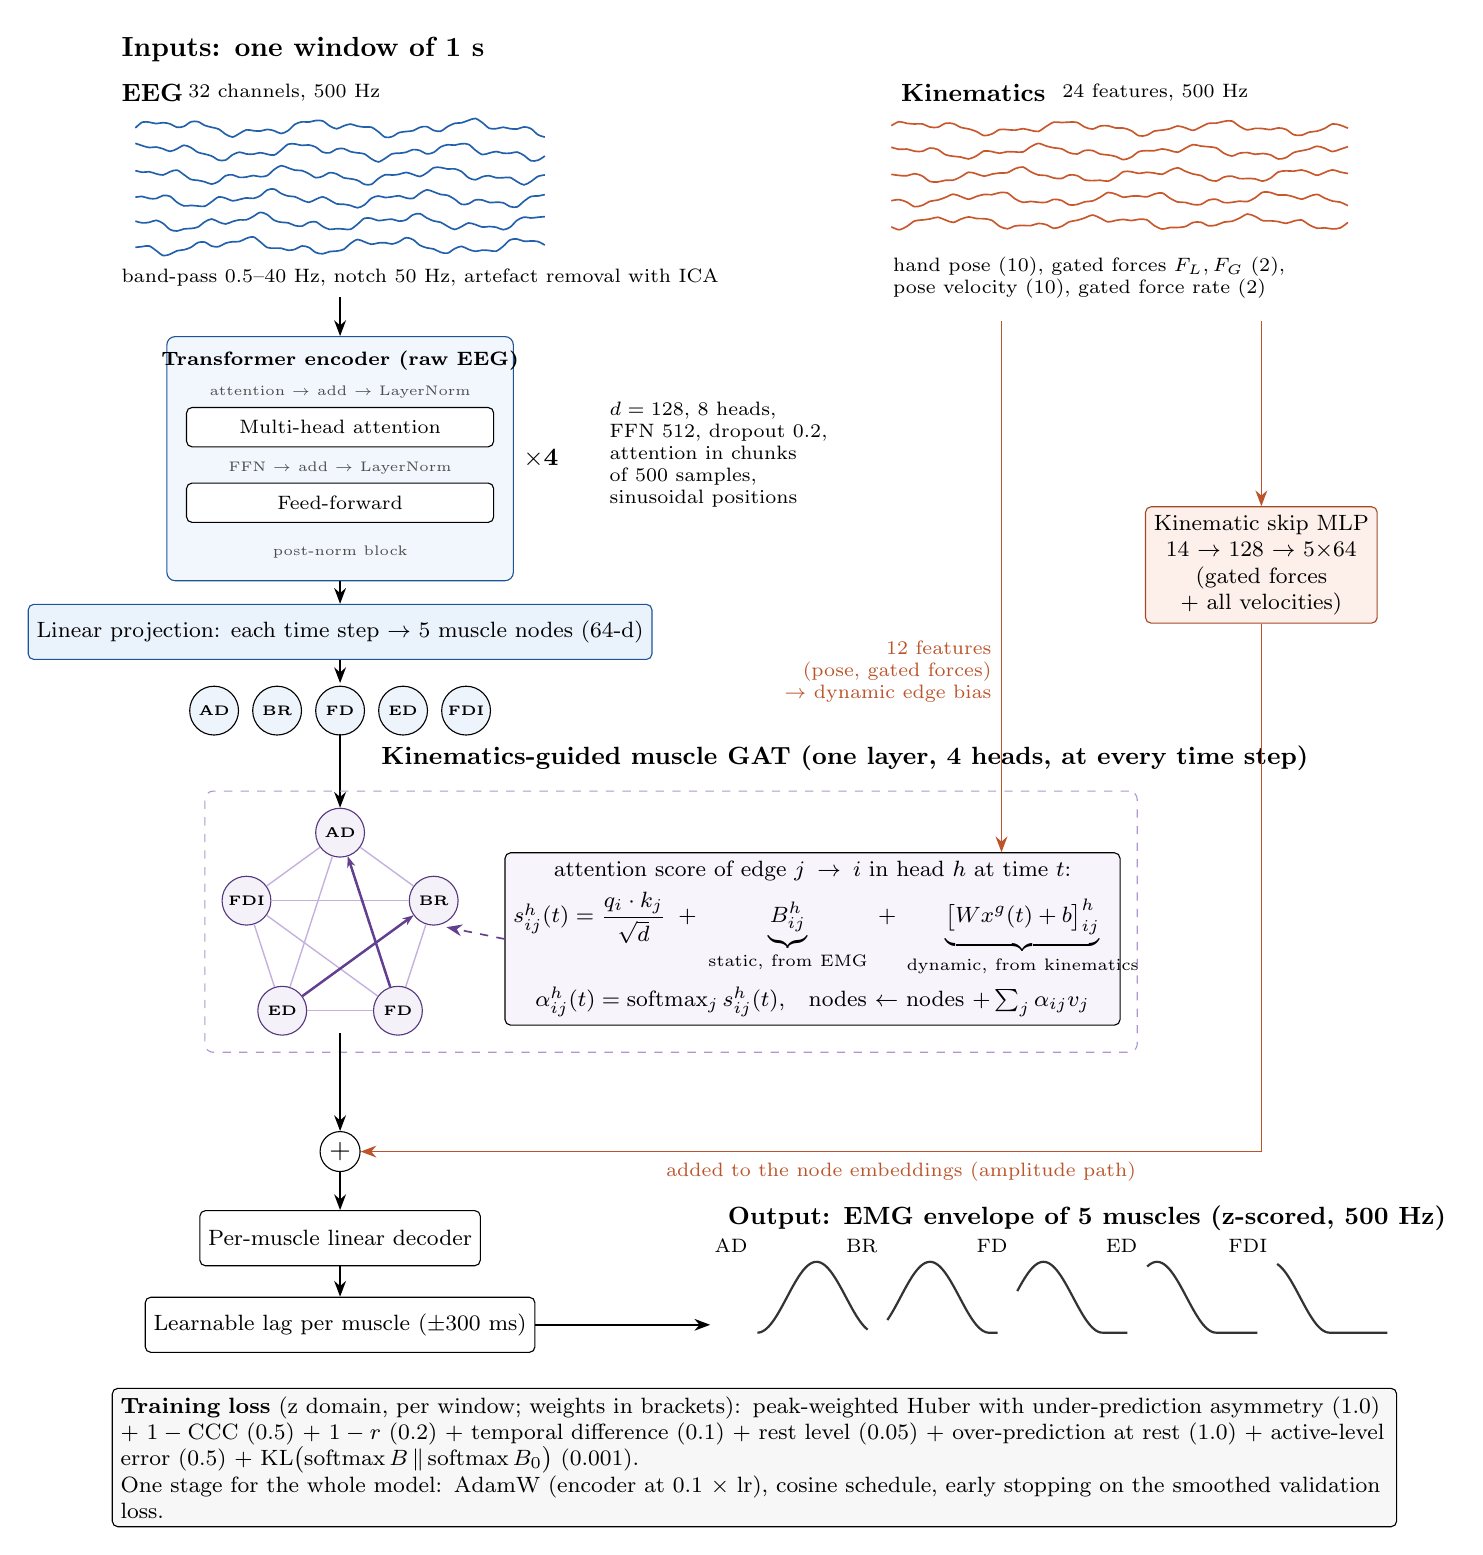
\begin{tikzpicture}[font=\footnotesize]
% ================= inputs
\node[lab, font=\normalsize\bfseries, anchor=west] at (-0.3,0.55) {Inputs: one window of 1 s};
\node[lab, font=\small\bfseries, anchor=west] at (-0.3,0.0) {EEG};
\node[lab, anchor=west] at (0.55,0.0) {32 channels, 500 Hz};
\foreach \k in {0,...,5}{\begin{scope}[shift={(0,-0.45-0.3*\k)}]\sig{0}{5.2}{0.12}{eegc!80!black}{40*\k}\end{scope}}
\node[lab, anchor=west] at (-0.3,-2.35) {band-pass 0.5--40 Hz, notch 50 Hz, artefact removal with ICA};
\node[lab, font=\small\bfseries, anchor=west] at (9.6,0.0) {Kinematics};
\node[lab, anchor=west] at (11.65,0.0) {24 features, 500 Hz};
\foreach \k in {0,...,4}{\begin{scope}[shift={(9.6,-0.45-0.3*\k)}]\sig{0}{5.8}{0.1}{kinc!85!black}{70*\k+15}\end{scope}}
\node[lab, anchor=west, align=left] at (9.5,-2.35) {hand pose (10), gated forces $F_L, F_G$ (2),\\ pose velocity (10), gated force rate (2)};

% ================= EEG path
\tblock{enc}{2.6,-4.65}{4.4cm}{Transformer encoder (raw EEG)}{4}{eegc}{attention $\to$ add $\to$ LayerNorm}{FFN $\to$ add $\to$ LayerNorm}{post-norm block}
\node[lab, anchor=west, align=left] at (5.9,-4.6) {$d=128$, 8 heads,\\ FFN 512, dropout 0.2,\\ attention in chunks\\ of 500 samples,\\ sinusoidal positions};
\draw[arr] (2.6,-2.6)--(enc.north);
\node[ebox, align=center] (proj) at (2.6,-6.85) {Linear projection: each time step $\to$ 5 muscle nodes (64-d)};
\draw[arr] (enc.south)--(proj.north);
\foreach \m/\k in {AD/0,BR/1,FD/2,ED/3,FDI/4}{\node[mnode, fill=eegc!8] (n\m) at (1.0+0.8*\k,-7.85) {\m};}
\draw[arr] (proj.south)--(2.6,-7.5);

% ================= kinematics-guided muscle GAT
\node[lab, font=\small\bfseries, anchor=west] at (3.0,-8.45) {Kinematics-guided muscle GAT (one layer, 4 heads, at every time step)};
\musclegraph{g}{2.6,-10.65}{1.25}{intc}
\draw[arr] (2.6,-8.15)--(gAD.north);
\node[box, fill=intc!6, align=center, text width=7.6cm] (score) at (8.6,-10.75) {attention score of edge $j\to i$ in head $h$ at time $t$:\\[3pt]
  \mbox{$s^{h}_{ij}(t)=\dfrac{q_i\cdot k_j}{\sqrt{d}}\;+\;\underbrace{B^{h}_{ij}}_{\text{static, from EMG}}\;+\;\underbrace{\big[W x^{g}(t)+b\big]^{h}_{ij}}_{\text{dynamic, from kinematics}}$}\\[3pt]
  \mbox{$\alpha^{h}_{ij}(t)=\mathrm{softmax}_j\, s^{h}_{ij}(t)$,\quad nodes $\leftarrow$ nodes $+\sum_j \alpha_{ij} v_j$}};
\draw[darr, intc!80!black] (score.west)--(3.95,-10.6);
\node[grp, draw=intc!60, fit=(gAD)(gFD)(gED)(gFDI)(gBR)(score)] (gatbox) {};

% ================= kinematic paths
\coordinate (kx) at (11.0,0);
\draw[arr, kinc!80!black] (11.0,-2.9)--(score.north -| kx) node[lab, pos=0.66, anchor=east, align=right]{12 features\\ (pose, gated forces)\\ $\to$ dynamic edge bias};
\node[kbox, align=center] (skip) at (14.3,-6.0) {Kinematic skip MLP\\ 14 $\to$ 128 $\to$ 5$\times$64\\ (gated forces\\ + all velocities)};
\draw[arr, kinc!80!black] (14.3,-2.9)--(skip.north);
\node[circle, draw, inner sep=1.5pt, fill=white, font=\normalsize] (plus) at (2.6,-13.45) {$+$};
\draw[arr] (2.6,-11.95)--(plus.north);
\draw[arr, kinc!80!black] (skip.south)|-(plus.east) node[lab, pos=0.7, below]{added to the node embeddings (amplitude path)};

% ================= decoder and output
\node[box, align=center] (dec) at (2.6,-14.55) {Per-muscle linear decoder};
\node[box, align=center] (lag) at (2.6,-15.65) {Learnable lag per muscle ($\pm$300 ms)};
\draw[arr] (plus)--(dec); \draw[arr] (dec)--(lag);
\node[lab, font=\small\bfseries, anchor=west] at (7.4,-14.3) {Output: EMG envelope of 5 muscles (z-scored, 500 Hz)};
\foreach \m/\k in {AD/0,BR/1,FD/2,ED/3,FDI/4}{
  \node[lab, anchor=east] at (7.9+1.65*\k,-14.65) {\m};
  \begin{scope}[shift={(7.9+1.65*\k,-15.75)}]\env{0}{1.4}{0.9}{black!80}{25*\k}\end{scope}}
\draw[arr] (lag.east)--(7.3,-15.65);

% ================= loss
\node[box, fill=black!3, anchor=north west, align=left, text width=16.1cm] (loss) at (-0.3,-16.45) {\textbf{Training loss} (z domain, per window; weights in brackets): peak-weighted Huber with under-prediction asymmetry (1.0) + $1-\mathrm{CCC}$ (0.5) + $1-r$ (0.2) + temporal difference (0.1) + rest level (0.05) + over-prediction at rest (1.0) + active-level error (0.5) + $\mathrm{KL}\big(\mathrm{softmax}\,B\,\|\,\mathrm{softmax}\,B_0\big)$ (0.001).\\ One stage for the whole model: AdamW (encoder at 0.1 $\times$ lr), cosine schedule, early stopping on the smoothed validation loss.};
\end{tikzpicture}}\end{latin}

\caption{نمای کلی مدل پایه \lr{KG-GT} از ورودی تا خروجی. پنجره‌ی یک‌ثانیه‌ای \lr{EEG} از \lr{encoder} \lr{Transformer} (چهار بلوک توجه و \lr{feed-forward}) می‌گذرد، هر گام زمانی به پنج گره‌ی عضله تصویر می‌شود و یک لایه‌ی \lr{graph attention} بین عضله‌ها پیام جابه‌جا می‌کند. سینماتیک از دو راه وارد می‌شود: دوازده ویژگی امتیاز یال‌های گراف را تغییر می‌دهند (خط نارنجی) و چهارده ویژگی از یک بزرگراه مستقیم به بردار گره‌ها اضافه می‌شوند. رمزگشای هر عضله و تأخیر آموختنی پوش \lr{EMG} را می‌سازند. کادر پایین هشت جزء \lr{loss function} را با وزن‌هایشان نشان می‌دهد.}
\label{fig:base-arch}
\end{figure}

\subsection{\lr{loss function}}

هزینه در حوزه‌ی استانداردشده ($z$) و روی هر پنجره حساب می‌شود و هشت جزء دارد. با $y_{tc}$ هدف و $\hat y_{tc}$ پیش‌بینی در زمان $t$ و عضله‌ی $c$، و $u_{tc}=(y_{tc}-\min_t y)/(\max_t y-\min_t y)$ سطح نسبی فعالیت در همان پنجره:

\begin{itemize}
\item \textbf{خطای وزن‌دار قله‌ها} (وزن \lr{۱٫۰}): $L_{peak}=\operatorname{mean}\big[w_c\,(1+\alpha u^2)\,(1+(a-1)\,\mathbb{I}[\hat y<y]\,u)\,\rho_\delta(\hat y-y)\big]$ با $\alpha=3$، ضریب عدم‌تقارن $a=1.5$ (کم‌برآوردی در قله‌ها گران‌تر است)، $\rho_\delta$ دو برابر تابع هوبر با $\delta=2.5$ و $w_c$ وزن هر عضله (عکس صدک ۹۵ هدف، با میانگین ۱).
\item \textbf{\lr{concordance correlation (CCC)}} (وزن \lr{۰٫۵}): $L_{ccc}=1-\mathrm{CCC}$ برای هر پنجره و عضله.
\item \textbf{\lr{Pearson correlation}} (وزن \lr{۰٫۲}): $L_{r}=1-r$.
\item \textbf{تفاضل زمانی} (وزن \lr{۰٫۱}): اختلاف تفاضل‌های مرتبه‌ی اول پیش‌بینی و هدف.
\item \textbf{استراحت} (وزن \lr{۰٫۰۵}): $L_{rest}=\operatorname{mean}\big[m\,|\hat y-\min_t y|\big]$ که $m$ نقاطی است که هدف در ۱۵ درصد پایینیِ بازه‌ی پنجره است.
\item \textbf{بیش‌برآوردی در استراحت} (وزن \lr{۱٫۰}): $\operatorname{mean}\big[m\,w_c\,\mathrm{relu}(\hat y-y)^2\big]$.
\item \textbf{سطح فعالیت} (وزن \lr{۰٫۵}): خطای نسبی میانگین سطح فعالیت (بالاتر از کمینه‌ی پنجره) در نقاط غیراستراحت، با هوبر هموار و همان عدم‌تقارن $a$.
\item \textbf{تنظیم گراف} (وزن \lr{۰٫۰۰۱}): واگرایی $\mathrm{KL}\big(\operatorname{softmax}(B)\,\|\,\operatorname{softmax}(B_0)\big)$ که \lr{bias} ایستای یال‌ها را نزدیک مقدار اولیه‌ی برگرفته از همبستگی \lr{EMG} نگه می‌دارد.
\end{itemize}

\subsection{آموزش}

\lr{optimizer} \lr{AdamW} با \lr{learning rate} $10^{-3}$ برای گراف و \lr{decoder} و یک‌دهم آن برای \lr{encoder}، \lr{weight decay} \lr{۰٫۰۱}، ۵ دوره \lr{warm-up} و سپس \lr{cosine decay}، \lr{batch size} ۳۲ با انباشت دو گام، \lr{mixed precision} و حداکثر ۲۰۰ دوره. \lr{early stopping} وقتی است که میانگین پنج‌دوره‌ای خطای \lr{validation} ۲۰ دوره بهتر نشود.

\subsection{نتایج مدل پایه}

جدول~\ref{tab:base-subj} نتیجه‌ی هر شرکت‌کننده و جدول~\ref{tab:base-musc} نتیجه‌ی هر عضله را نشان می‌دهد. میانگین \lr{VAF} برابر \lr{۷۲٫۲} درصد و میانگین \lr{r} برابر \lr{۰٫۸۵۱} است. سه عضله‌ی \lr{AD}، \lr{BR} و \lr{ED} خوب پیش‌بینی می‌شوند و \lr{FD} و \lr{FDI} ضعیف‌ترند. میانگین \lr{height ratio} \lr{۰٫۹۷۳} است؛ یعنی دامنه به‌طور کلی درست است، اما سطح بیش‌برآورد (\lr{۰٫۱۳۸}) از سطح کم‌برآورد (\lr{۰٫۰۸۹}) بیشتر است.

\begin{table}[htbp]
\centering
\small
\caption{مدل پایه \lr{KG-GT} (\lr{main\_1stage})، سری‌های آزمون: میانگین روی پنج عضله برای هر شرکت‌کننده.}
\label{tab:base-subj}
\begin{tabular}{ccccc}
\toprule
شرکت‌کننده & \lr{r} & \lr{CCC} & \lr{VAF} (\%) & \lr{height ratio} \\
\midrule
\lr{P1} & \lr{۰٫۸۹۱} & \lr{۰٫۸۶۹} & \lr{۷۹٫۰} & \lr{۰٫۹۲۲} \\
\lr{P2} & \lr{۰٫۸۷۲} & \lr{۰٫۸۶۸} & \lr{۷۵٫۲} & \lr{۰٫۹۷۷} \\
\lr{P3} & \lr{۰٫۸۱۱} & \lr{۰٫۷۸۲} & \lr{۶۷٫۵} & \lr{۰٫۹۹۴} \\
\lr{P4} & \lr{۰٫۸۸۰} & \lr{۰٫۸۷۱} & \lr{۷۶٫۰} & \lr{۱٫۰۳۱} \\
\lr{P5} & \lr{۰٫۷۷۷} & \lr{۰٫۷۳۶} & \lr{۶۳٫۵} & \lr{۰٫۹۲۷} \\
\lr{P6} & \lr{۰٫۸۶۵} & \lr{۰٫۸۳۱} & \lr{۷۴٫۷} & \lr{۰٫۹۹۴} \\
\lr{P7} & \lr{۰٫۸۹۹} & \lr{۰٫۸۷۰} & \lr{۷۹٫۱} & \lr{۰٫۸۹۸} \\
\lr{P8} & \lr{۰٫۷۶۴} & \lr{۰٫۷۴۲} & \lr{۵۴٫۳} & \lr{۱٫۰۴۷} \\
\lr{P9} & \lr{۰٫۸۹۷} & \lr{۰٫۸۹۲} & \lr{۷۹٫۳} & \lr{۰٫۹۹۳} \\
\lr{P10} & \lr{۰٫۸۷۱} & \lr{۰٫۸۶۵} & \lr{۷۴٫۹} & \lr{۰٫۹۹۱} \\
\lr{P11} & \lr{۰٫۸۵۸} & \lr{۰٫۸۴۸} & \lr{۷۳٫۶} & \lr{۰٫۹۵۴} \\
\lr{P12} & \lr{۰٫۸۳۲} & \lr{۰٫۸۱۴} & \lr{۶۹٫۸} & \lr{۰٫۹۴۹} \\
\midrule
\textbf{میانگین} & \lr{۰٫۸۵۱} & \lr{۰٫۸۳۲} & \lr{۷۲٫۲} & \lr{۰٫۹۷۳} \\
\bottomrule
\end{tabular}
\end{table}

\begin{table}[htbp]
\centering
\small
\caption{مدل پایه، میانگین روی ۱۲ شرکت‌کننده برای هر عضله.}
\label{tab:base-musc}
\begin{tabular}{ccccc}
\toprule
عضله & \lr{r} & \lr{VAF} (\%) & سطح بیش‌برآورد & سطح کم‌برآورد \\
\midrule
\lr{AD} & \lr{۰٫۹۳۴} & \lr{۸۵٫۹} & \lr{۰٫۱۵۴} & \lr{۰٫۰۷۴} \\
\lr{BR} & \lr{۰٫۸۹۷} & \lr{۷۹٫۶} & \lr{۰٫۱۱۸} & \lr{۰٫۰۶۸} \\
\lr{FD} & \lr{۰٫۷۰۴} & \lr{۴۹٫۵} & \lr{۰٫۱۳۲} & \lr{۰٫۰۸۰} \\
\lr{ED} & \lr{۰٫۹۱۶} & \lr{۸۲٫۴} & \lr{۰٫۱۳۷} & \lr{۰٫۰۸۵} \\
\lr{FDI} & \lr{۰٫۸۰۶} & \lr{۶۳٫۷} & \lr{۰٫۱۴۸} & \lr{۰٫۱۳۸} \\
\bottomrule
\end{tabular}
\end{table}


شکل~\ref{fig:base_triptych_P1.png} نمونه‌ای از شکل تفسیری مدل پایه است: پیش‌بینی در برابر هدف، تفکیک دقیق خروجی به مسیر گراف و مسیر \lr{kinematic skip highway}، و تغییر توجه \lr{muscle graph} نسبت به حالت استراحت. در این شکل دیده می‌شود که شکل و زمان‌بندی جهش‌ها تقریباً همه از \lr{kinematic skip highway} (منحنی نارنجی پنل ۲) می‌آیند.

\fig{base_triptych_P1.png}{0.92}{مدل پایه، شرکت‌کننده‌ی \lr{P1}، سری آزمون ۴، ثانیه‌ی ۳۰ تا ۴۰. پنل ۱: پوش واقعی و پیش‌بینی. پنل ۲: تفکیک دقیق خروجی به مسیر \lr{EEG} و گراف (بنفش) و مسیر \lr{kinematic skip highway} (نارنجی). پنل ۳: تغییر توجه \lr{muscle graph} نسبت به میانگین استراحت.}

\fig{base_magnitude.png}{0.95}{گزارش دامنه‌ی مدل پایه برای شرکت‌کننده‌های \lr{P1} تا \lr{P6}. چپ: \lr{height ratio} فعالیت برای هر عضله، یک ستون برای هر سری آزمون و یک ستون خاکستری برای همه‌ی سری‌ها (خط‌چین = ۱). راست: سطح استراحت پیش‌بینی در برابر هدف. جدول~\ref{tab:base-subj} همین اعداد را برای هر ۱۲ نفر دارد.}

\subsubsection*{سهم \lr{EEG} در مدل پایه}

جدول~\ref{tab:base-abl} نتیجه‌ی حذف ورودی را نشان می‌دهد. اگر سینماتیک صفر شود، \lr{r} از \lr{۰٫۸۵۱} به \lr{۰٫۰۳۵} می‌افتد؛ اگر \lr{EEG} بین پنجره‌ها جابه‌جا شود، \lr{r} حتی کمی بالا می‌رود (\lr{۰٫۸۵۵}). یعنی پیش‌بینی مدل پایه تقریباً تماماً از سینماتیک است و \lr{EEG} در عمل یک ورودیِ بی‌اثر است.

\begin{table}[htbp]
\centering
\small
\caption{\lr{input ablation} در مدل پایه: ضریب همبستگی \lr{r} وقتی یک ورودی صفر یا جابه‌جا می‌شود.}
\label{tab:base-abl}
\begin{tabular}{ccccc}
\toprule
شرکت‌کننده & کامل & سینماتیک صفر & سینماتیک جابه‌جا & \lr{EEG} جابه‌جا \\
\midrule
\lr{P1} & \lr{۰٫۸۹۱} & \lr{−۰٫۰۱۰} & \lr{۰٫۸۱۶} & \lr{۰٫۸۹۴} \\
\lr{P2} & \lr{۰٫۸۷۲} & \lr{۰٫۱۱۱} & \lr{۰٫۸۳۸} & \lr{۰٫۸۷۴} \\
\lr{P3} & \lr{۰٫۸۱۱} & \lr{۰٫۰۶۸} & \lr{۰٫۷۴۰} & \lr{۰٫۸۱۶} \\
\lr{P4} & \lr{۰٫۸۸۰} & \lr{۰٫۰۵۱} & \lr{۰٫۸۲۶} & \lr{۰٫۸۸۵} \\
\lr{P5} & \lr{۰٫۷۷۷} & \lr{۰٫۰۳۹} & \lr{۰٫۷۴۰} & \lr{۰٫۷۸۰} \\
\lr{P6} & \lr{۰٫۸۶۵} & \lr{۰٫۰۱۱} & \lr{۰٫۸۳۲} & \lr{۰٫۸۶۸} \\
\lr{P7} & \lr{۰٫۸۹۹} & \lr{۰٫۱۶۹} & \lr{۰٫۸۷۲} & \lr{۰٫۹۰۲} \\
\lr{P8} & \lr{۰٫۷۶۴} & \lr{۰٫۰۳۵} & \lr{۰٫۶۶۳} & \lr{۰٫۷۷۱} \\
\lr{P9} & \lr{۰٫۸۹۷} & \lr{۰٫۰۰۶} & \lr{۰٫۸۶۴} & \lr{۰٫۸۹۹} \\
\lr{P10} & \lr{۰٫۸۷۱} & \lr{−۰٫۰۹۶} & \lr{۰٫۸۱۲} & \lr{۰٫۸۷۷} \\
\lr{P11} & \lr{۰٫۸۵۸} & \lr{۰٫۰۱۵} & \lr{۰٫۸۳۰} & \lr{۰٫۸۶۵} \\
\lr{P12} & \lr{۰٫۸۳۲} & \lr{۰٫۰۱۹} & \lr{۰٫۷۸۴} & \lr{۰٫۸۳۴} \\
\midrule
\textbf{میانگین} & \lr{۰٫۸۵۱} & \lr{۰٫۰۳۵} & \lr{۰٫۸۰۱} & \lr{۰٫۸۵۵} \\
\bottomrule
\end{tabular}
\end{table}

\fig{base_ablation.png}{0.8}{\lr{input ablation} در مدل پایه برای \lr{P1} تا \lr{P6}: میانگین \lr{r} روی پنج عضله برای مدل کامل، سینماتیک صفر، سینماتیک جابه‌جاشده در زمان و \lr{EEG} جابه‌جاشده در زمان. جدول~\ref{tab:base-abl} هر ۱۲ نفر را دارد.}

برای اینکه این نتیجه به ساختار مدل پایه وابسته نباشد، آزمایش جداگانه‌ای انجام شد (جدول~\ref{tab:base-res}): ابتدا مدلی فقط با سینماتیک آموزش دید و سپس \lr{EEG} فقط برای پیش‌بینی باقی‌مانده‌ی آن به کار رفت. مدل فقط‌سینماتیک به \lr{VAF} برابر \lr{۷۵٫۵} درصد رسید (بیشتر از مدل پایه‌ی کامل) و افزودن \lr{EEG} آن را به‌طور متوسط \lr{۰٫۷۴} واحد بدتر کرد. فقط ۴ خانه از ۶۰ خانه (شرکت‌کننده × عضله) بهبود معنادار داشتند که نزدیک به عددی است که از شانس انتظار می‌رود (۳ خانه).

\begin{table}[htbp]
\centering
\small
\caption{\lr{residual experiment} روی مدل پایه (شاخه \lr{KG-GT-CUDA}): مدل فقط‌سینماتیک در برابر مدلی که \lr{EEG} را روی باقی‌مانده‌ی آن آموزش می‌دهد. ستون آخر: تعداد خانه‌های (سری × عضله) با \lr{p} آزمون جابه‌جایی کمتر از \lr{۰٫۰۵}.}
\label{tab:base-res}
\begin{tabular}{cccccc}
\toprule
شرکت‌کننده & \lr{VAF} فقط سینماتیک & \lr{VAF} کامل & $\Delta$\lr{VAF} & \lr{r} باقی‌مانده & خانه‌های معنادار \\
\midrule
\lr{P1} & \lr{۸۳٫۲} & \lr{۸۲٫۴} & \lr{−۰٫۷۳} & \lr{۰٫۰۲۵} & \lr{۰} از \lr{۵} \\
\lr{P2} & \lr{۷۶٫۸} & \lr{۷۶٫۳} & \lr{−۰٫۵۷} & \lr{۰٫۰۵۳} & \lr{۰} از \lr{۵} \\
\lr{P3} & \lr{۷۰٫۰} & \lr{۶۹٫۷} & \lr{−۰٫۲۸} & \lr{۰٫۰۲۰} & \lr{۱} از \lr{۵} \\
\lr{P4} & \lr{۷۹٫۵} & \lr{۷۹٫۲} & \lr{−۰٫۳۳} & \lr{۰٫۰۸۸} & \lr{۰} از \lr{۵} \\
\lr{P5} & \lr{۶۶٫۳} & \lr{۶۴٫۲} & \lr{−۲٫۱۴} & \lr{۰٫۰۴۳} & \lr{۰} از \lr{۵} \\
\lr{P6} & \lr{۷۷٫۰} & \lr{۷۶٫۵} & \lr{−۰٫۵۶} & \lr{۰٫۰۰۳} & \lr{۰} از \lr{۵} \\
\lr{P7} & \lr{۸۳٫۴} & \lr{۸۳٫۱} & \lr{−۰٫۲۸} & \lr{۰٫۰۵۸} & \lr{۱} از \lr{۵} \\
\lr{P8} & \lr{۶۱٫۸} & \lr{۶۰٫۷} & \lr{−۱٫۱۱} & \lr{۰٫۰۴۶} & \lr{۱} از \lr{۵} \\
\lr{P9} & \lr{۸۰٫۷} & \lr{۸۰٫۱} & \lr{−۰٫۶۸} & \lr{۰٫۰۳۲} & \lr{۰} از \lr{۵} \\
\lr{P10} & \lr{۷۸٫۰} & \lr{۷۷٫۹} & \lr{−۰٫۱۳} & \lr{۰٫۰۹۸} & \lr{۱} از \lr{۵} \\
\lr{P11} & \lr{۷۷٫۳} & \lr{۷۵٫۷} & \lr{−۱٫۵۹} & \lr{۰٫۰۱۸} & \lr{۰} از \lr{۵} \\
\lr{P12} & \lr{۷۱٫۷} & \lr{۷۱٫۲} & \lr{−۰٫۴۹} & \lr{۰٫۰۰۰} & \lr{۰} از \lr{۵} \\
\midrule
\textbf{میانگین} & \lr{۷۵٫۵} & \lr{۷۴٫۷} & \lr{−۰٫۷۴} & \lr{۰٫۰۴۰} & \lr{۴} از \lr{۶۰} \\
\bottomrule
\end{tabular}
\end{table}

\fig{base_residual_dvaf.png}{0.85}{\lr{residual experiment} روی مدل پایه برای \lr{P1} تا \lr{P6}. چپ: \lr{VAF} هر عضله برای مدل فقط‌سینماتیک (نارنجی) و همان مدل به‌علاوه‌ی \lr{EEG} روی باقی‌مانده (آبی). راست: تغییر \lr{VAF} (ستون آبی) روی \lr{null distribution} با \lr{EEG} پنجره‌ای دیگر (نوار خاکستری، میانگین $\pm$ دو انحراف معیار) و $p$ تجربی. جدول~\ref{tab:base-res} هر ۱۲ نفر را دارد.}

\section{کاستی‌های مدل پایه}
\label{sec:gaps}

\paragraph{سهم \lr{EEG} قابل‌سنجش نیست.} مدل پایه یک خروجی دارد و \lr{EEG} و سینماتیک درون یک گراف با هم ترکیب می‌شوند. وقتی سینماتیک این‌قدر قوی است، بهینه‌سازی راه کوتاه را انتخاب می‌کند و \lr{EEG} کنار می‌رود. با یک خروجی نمی‌توان هم دقت را گزارش کرد و هم ادعای علوم اعصاب («\lr{EEG} حرکت را رمز می‌کند») را آزمود.

\paragraph{بافت زمانی کوتاه.} پنجره‌ی یک‌ثانیه‌ای از یک بلندکردن کامل (چند ثانیه) کوتاه‌تر است. مدل نمی‌بیند جسم چند ثانیه است نگه داشته شده یا بلندکردن قبلی چقدر سنگین بود.

\paragraph{خطاهای دامنه وابسته به وزن جسم.} \lr{height ratio} میانگین درست است، اما وزن‌های سبک و متوسط ۴ تا ۱۱ درصد بیش‌برآورد می‌شوند و همبستگی سطح فعالیت بین بلندکردن‌ها در یک وزن ثابت ضعیف است (برای \lr{AD} حدود \lr{۰٫۰۷}). ضریب ثابت بهترینِ هر سری فقط \lr{۱٫۳} واحد به \lr{VAF} اضافه می‌کند، پس مشکل یک مقیاس کلی نیست. مدل اطلاعاتی از تاریخچه‌ی بلندکردن‌ها ندارد.

\paragraph{هزینه‌ی پیچیده و جهت‌دار.} وزن‌دهی قله‌ها، عدم‌تقارن و ماسک استراحت در حوزه‌ی $z$ مدل را به سمت بیش‌برآوردی هل می‌دهند (سطح بیش‌برآورد بزرگ‌تر از کم‌برآورد). هشت جزء با هشت وزن، اثر هر کدام را سخت قابل‌ردیابی می‌کند.

\paragraph{سقف داده.} پیش‌بین هموار ایدئال (خودِ هدف با \lr{low-pass} ۲ هرتز) برای \lr{FD} فقط به ۷۴ درصد می‌رسد؛ بخشی از خطا در خود ثبت‌هاست و هیچ مدلی آن را جبران نمی‌کند (بخش~\ref{sec:v2-results}).

\paragraph{تفسیرپذیری محدود.} اطلاعات در مدل پایه از چند راه بین موقعیت‌ها جابه‌جا می‌شود: توجه تکه‌تکه، تأخیر آموختنی (یک کانولوشن)، \lr{kinematic skip highway} و گراف. لایه‌های گراف پس‌نرمال‌اند و \lr{encoder} هیچ \lr{recorder} توجهی ندارد. بنابراین \lr{rollout} یا \lr{attention flow} از ورودی تا خروجی تعریف‌پذیر نیست. شکل تفسیری مدل پایه (شکل~\ref{fig:base_triptych_P1.png}) فقط توجه \lr{muscle graph} را نشان می‌دهد که توجه \lr{EEG} نیست.

\FloatBarrier
\section{چرا \lr{v2}}
\label{sec:why}

\lr{v2} برای رفع کاستی‌های بخش~\ref{sec:gaps} طراحی شد. مهم‌ترین تغییر این است که مدل به‌جای یک خروجی، سه خروجی جدا دارد:
\begin{itemize}
\item \textbf{\lr{K}} فقط از سینماتیک و تاریخچه‌ی بلندکردن‌ها ساخته می‌شود. می‌گوید سینماتیک به‌تنهایی چقدر خوب پیش‌بینی می‌کند.
\item \textbf{\lr{E}} فقط از \lr{EEG} ساخته می‌شود. می‌گوید \lr{EEG} به‌تنهایی چه چیزی از فعالیت عضله را در خود دارد.
\item \textbf{\lr{F}} همان \lr{K} است به‌علاوه‌ی یک اصلاح کوچک از \lr{EEG}. اگر \lr{F} از \lr{K} بهتر شود، \lr{EEG} چیزی دارد که سینماتیک ندارد.
\end{itemize}
با این سه خروجی، دو پرسشی که در مدل پایه با هم قاطی می‌شدند جدا می‌شوند. جدول~\ref{tab:why} بقیه‌ی تغییرها را کنار کاستی متناظر می‌گذارد.

\begin{table}[htbp]
\centering\small
\caption{کاستی‌های مدل پایه و پاسخ \lr{v2} به هر کدام.}
\label{tab:why}
\begin{tabular}{p{0.38\textwidth}p{0.52\textwidth}}
\toprule
کاستی مدل پایه & تصمیم در \lr{v2} \\
\midrule
یک خروجی؛ سهم \lr{EEG} را نمی‌توان جدا کرد & سه خروجی جدا: \lr{K} (سینماتیک)، \lr{E} (فقط \lr{EEG})، \lr{F} (\lr{K} به‌علاوه‌ی اصلاح \lr{gated} از \lr{EEG})؛ \lr{K} از \lr{E} و \lr{F} هیچ گرادیانی نمی‌گیرد \\
پنجره‌ی یک‌ثانیه‌ای & \lr{tokens} ۵۰ هرتز و پنجره‌ی ۸ ثانیه‌ای (۴۰۰ \lr{tokens}) \\
بی‌خبری از بلندکردن‌های قبلی & هشت ویژگی تاریخچه از نیروها، فقط از گذشته و بدون \lr{EMG} \\
\lr{loss function} هشت‌جزئی و یک‌طرفه در حوزه‌ی $z$ & حوزه‌ی جذر دامنه و \lr{loss function} چهارجزئی، بدون وزن اضافه‌ی قله و جزء استراحت \\
\lr{EEG} خام در حوزه‌ی زمان & \lr{band power} در چهار باند برای هر الکترود، به‌صورت گرافی از الکترودها \\
اطلاعات از چند نوع لایه جابه‌جا می‌شود؛ \lr{rollout} تعریف‌پذیر نیست & قاعده‌ی «یک مخلوط‌کننده»: فقط لایه‌های توجه اطلاعات را بین موقعیت‌ها جابه‌جا می‌کنند و همه‌شان ثبت می‌شوند \\
همه‌چیز با هم آموزش می‌بیند و با هم متوقف می‌شود & هر جریان \lr{optimizer} و توقف خودش را دارد؛ جریانی که دیگر بهتر نمی‌شود در بهترین نقطه‌اش \lr{freeze} می‌شود \\
\bottomrule
\end{tabular}
\end{table}

\lr{v2} از سه جهت بهتر از مدل پایه است.
\begin{enumerate}
\item \textbf{دقت.} \lr{K} در هر ۱۲ شرکت‌کننده \lr{VAF} بالاتری از مدل پایه دارد (بخش~\ref{sec:v2-results}).
\item \textbf{پرسش علمی روشن.} «آیا \lr{EEG} چیزی بیش از سینماتیک دارد؟» با مقایسه‌ی \lr{F} و \lr{K} و با \lr{residual test} جواب می‌گیرد. «آیا \lr{EEG} به‌تنهایی حرکت را رمز می‌کند؟» با \lr{E} جواب می‌گیرد.
\item \textbf{تفسیرپذیری.} برای هر عدد خروجی می‌توان دنبال کرد که از کدام ورودی‌ها و از کدام لایه‌ها آمده است.
\end{enumerate}

\FloatBarrier
\section{مدل \lr{v2}}
\label{sec:v2}

شکل~\ref{fig:v2-arch} کل مدل را نشان می‌دهد. مدل دو «جریان» مستقل دارد که هر کدام یک خروجی می‌سازند: جریان سینماتیک \lr{K} را و جریان \lr{EEG} \lr{E} را. یک ماژول کوچک سوم (\lr{fusion}) این دو را برای ساختن \lr{F} به هم وصل می‌کند. در ادامه اول ورودی‌ها و خروجی‌ها، بعد اجزای مدل و در آخر نحوه‌ی آموزش توضیح داده می‌شود.

\subsection{ورودی‌ها، \lr{tokens} و خروجی‌ها}

همه‌ی ورودی‌ها از پیش‌پردازش بخش~\ref{sec:preproc-v2} می‌آیند؛ اینجا فقط خلاصه‌شان آمده است.

\textbf{نرخ \lr{token}.} مدل پایه با ۵۰۰ نمونه در ثانیه کار می‌کرد. برای اینکه \lr{v2} بتواند ۸ ثانیه را یک‌جا ببیند، همه‌ی سیگنال‌ها با فیلتر ضدتداخل به ۵۰ هرتز برده می‌شوند. هر \lr{token} نماینده‌ی ۲۰ میلی‌ثانیه است و یک پنجره‌ی ۸ ثانیه‌ای ۴۰۰ \lr{token} دارد.

\textbf{سینماتیک} $X^{k}\in\mathbb{R}^{T\times24}$. همان ۲۴ ویژگی مدل پایه (وضعیت دست، دو نیروی \lr{gated} و سرعت‌هایشان)، استانداردشده با آماره‌های آموزش.

\textbf{تاریخچه} $X^{h}\in\mathbb{R}^{T\times8}$. این ویژگی‌ها به مدل می‌گویند تا این لحظه در سری چه گذشته است: آیا و چند بار جسم نگه داشته شده، چقدر از شروع سری و از آخرین نگه‌داشتن گذشته، و نیروهای آخرین نگه‌داشتن و میانگین همه‌ی نگه‌داشتن‌های قبلی. مدل فقط وقتی از یک نگه‌داشتن خبردار می‌شود که آن نگه‌داشتن تمام شده باشد؛ پس هیچ ویژگی‌ای از آینده خبر ندارد.

\textbf{\lr{EEG}} $X^{e}\in\mathbb{R}^{T\times32\times4}$. به‌جای موج خام، برای هر الکترود لگاریتم توان در چهار باند: تتا (۴ تا ۸ هرتز)، آلفا (۸ تا ۱۳)، بتا (۱۳ تا ۳۰) و گامای پایین (۳۰ تا ۴۰)، استانداردشده و بریده در $\pm5$.

\textbf{هدف در حوزه‌ی جذر.} برای هر عضله $s_c$ صدک ۹۵ پوش در داده‌ی آموزش است. مدل به‌جای خود پوش، جذر پوش نرمال‌شده را پیش‌بینی می‌کند:
\begin{equation}
u=\sqrt{y/s_c},\qquad \hat y=s_c\,\hat u^{2}.
\end{equation}
جذر قله‌های بلند را کوتاه‌تر و سطح‌های پایین را بازتر می‌کند. در نتیجه خطای قله‌ها و خطای استراحت وزن نزدیک‌تری می‌گیرند و دیگر لازم نیست قله‌ها را جداگانه وزن بدهیم یا جزء جداگانه‌ای برای استراحت بگذاریم.

\textbf{خروجی‌ها.} مدل برای هر \lr{token} و هر عضله سه عدد برمی‌گرداند:
\begin{equation}
K=K_{base}\odot g(X^{h}),\qquad E=\mathrm{E\text{-}stream}(X^{e}),\qquad F=\mathrm{relu}\big(K+F_{eeg}\big).
\end{equation}
$K_{base}$ پیش‌بینی جریان سینماتیک است و $g$ یک ضریب از تاریخچه که آن را کمی بزرگ یا کوچک می‌کند. $F_{eeg}$ اصلاحی است که \lr{EEG} به \lr{K} اضافه می‌کند. مدل این اجزا را هم جداگانه برمی‌گرداند تا بتوان سهم هر کدام را دید.

\begin{figure}[p]
\centering
% KG-GT v2: overview in the style of a paper's first figure (portrait).
\begin{latin}\resizebox{\textwidth}{!}{%
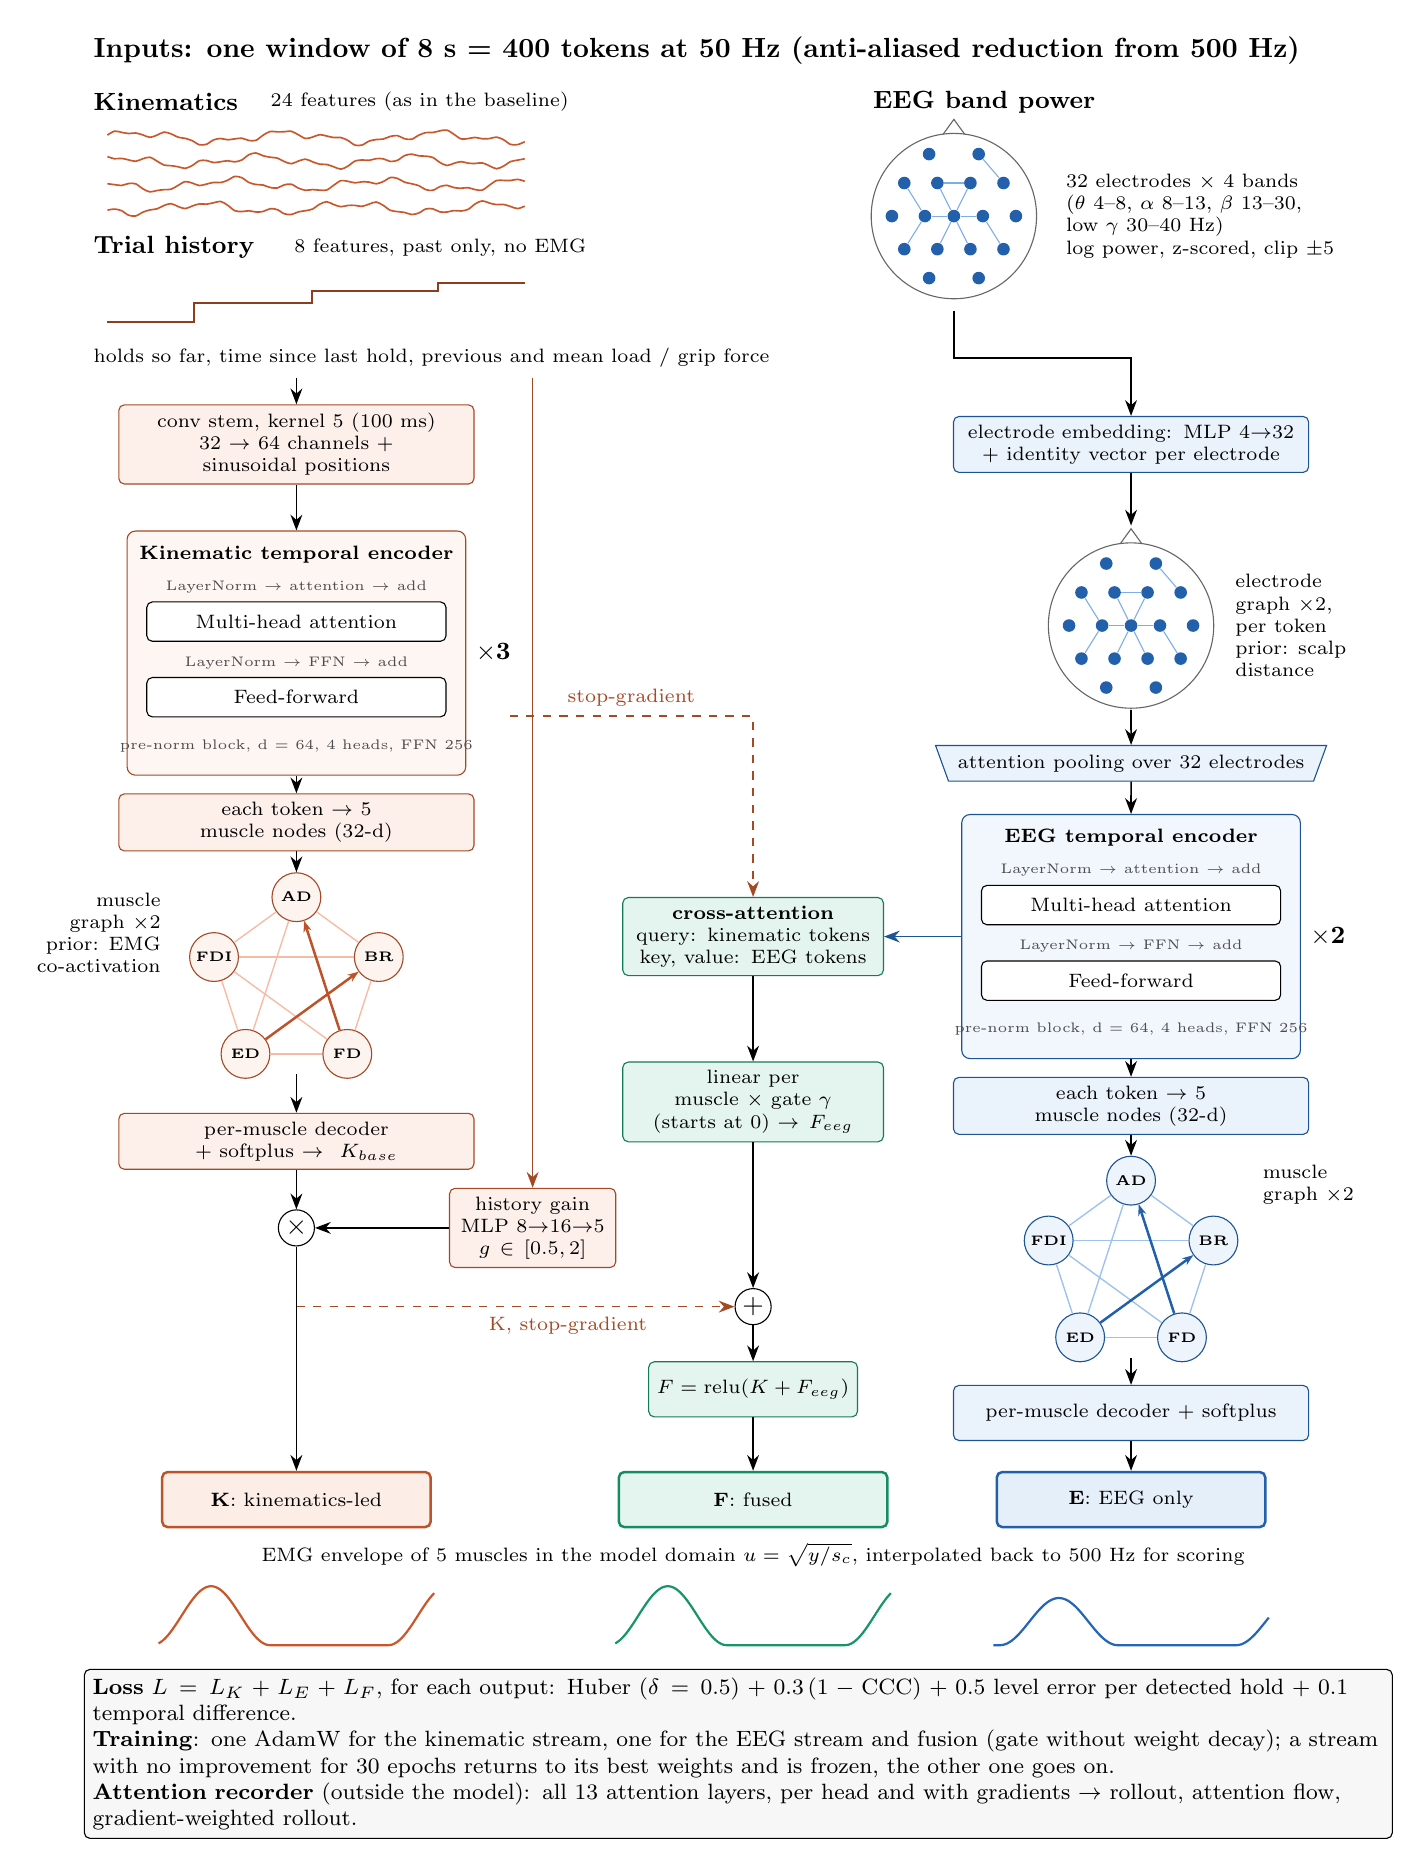
\begin{tikzpicture}[font=\footnotesize, box/.append style={font=\scriptsize}]
% ================= inputs
\node[lab, font=\normalsize\bfseries, anchor=west] at (-0.3,0.65) {Inputs: one window of 8 s = 400 tokens at 50 Hz (anti-aliased reduction from 500 Hz)};
\node[lab, font=\small\bfseries, anchor=west] at (-0.3,0.0) {Kinematics};
\node[lab, anchor=west] at (1.95,0.0) {24 features (as in the baseline)};
\foreach \k in {0,...,3}{\begin{scope}[shift={(0,-0.45-0.3*\k)}]\sig{0}{5.3}{0.1}{kinc!85!black}{70*\k+15}\end{scope}}
\node[lab, font=\small\bfseries, anchor=west] at (-0.3,-1.85) {Trial history};
\node[lab, anchor=west] at (2.25,-1.85) {8 features, past only, no EMG};
\draw[kinc!60!black, line width=0.8pt] (0,-2.8)--(1.1,-2.8)--(1.1,-2.55)--(2.6,-2.55)--(2.6,-2.4)--(4.2,-2.4)--(4.2,-2.3)--(5.3,-2.3);
\node[lab, anchor=west, align=left] at (-0.3,-3.25) {holds so far, time since last hold, previous and mean load / grip force};
\node[lab, font=\small\bfseries, anchor=west] at (9.6,0.0) {EEG band power};
\headgraph{h0}{10.75,-1.45}{1.05}
\node[lab, anchor=west, align=left] at (12.05,-1.45) {32 electrodes $\times$ 4 bands\\ ($\theta$ 4--8, $\alpha$ 8--13, $\beta$ 13--30,\\ low $\gamma$ 30--40 Hz)\\ log power, z-scored, clip $\pm$5};

% ================= kinematic stream (x = 2.4)
\node[kbox, align=center, text width=4.3cm] (stem) at (2.4,-4.35) {conv stem, kernel 5 (100 ms)\\ 32 $\to$ 64 channels + sinusoidal positions};
\draw[arr] (2.4,-3.5)--(stem.north);
\tblock{kenc}{2.4,-7.0}{4.3cm}{Kinematic temporal encoder}{3}{kinc}{LayerNorm $\to$ attention $\to$ add}{LayerNorm $\to$ FFN $\to$ add}{pre-norm block, d = 64, 4 heads, FFN 256}
\draw[arr] (stem.south)--(kenc.north);
\node[kbox, align=center, text width=4.3cm] (kproj) at (2.4,-9.15) {each token $\to$ 5 muscle nodes (32-d)};
\draw[arr] (kenc.south)--(kproj.north);
\musclegraph{km}{2.4,-11.2}{1.1}{kinc}
\draw[arr] (kproj.south)--(kmAD.north);
\node[lab, anchor=east, align=right] at (0.8,-10.55) {muscle\\ graph $\times$2\\ prior: EMG\\ co-activation};
\node[kbox, align=center, text width=4.3cm] (kdec) at (2.4,-13.2) {per-muscle decoder + softplus $\to K_{base}$};
\draw[arr] (2.4,-12.35)--(kdec.north);
\node[circle, draw, inner sep=1pt, fill=white, font=\normalsize] (times) at (2.4,-14.3) {$\times$};
\draw[arr] (kdec.south)--(times.north);
\node[kbox, align=center, text width=1.9cm] (gain) at (5.4,-14.3) {history gain\\ MLP 8$\to$16$\to$5\\ $g\in[0.5,2]$};
\draw[arr, kinc!70!black] (5.4,-3.5)--(gain.north);
\draw[arr] (gain.west)--(times.east);

% ================= EEG stream (x = 13.0)
\node[ebox, align=center, text width=4.3cm] (emb) at (13.0,-4.35) {electrode embedding: MLP 4$\to$32\\ + identity vector per electrode};
\draw[arr] (10.75,-2.65)--(10.75,-3.25)-|(emb.north);
\headgraph{h1}{13.0,-6.65}{1.05}
\draw[arr] (emb.south)--(13.0,-5.38);
\node[lab, anchor=west, align=left] at (14.2,-6.65) {electrode\\ graph $\times$2,\\ per token\\ prior: scalp\\ distance};
\node[trapezium, trapezium left angle=70, trapezium right angle=70, shape border rotate=180, draw=eegc!70!black, fill=eegc!10, align=center, minimum width=3.8cm, font=\scriptsize] (pool) at (13.0,-8.4) {attention pooling over 32 electrodes};
\draw[arr] (13.0,-7.72)--(pool.north);
\tblock{eenc}{13.0,-10.6}{4.3cm}{EEG temporal encoder}{2}{eegc}{LayerNorm $\to$ attention $\to$ add}{LayerNorm $\to$ FFN $\to$ add}{pre-norm block, d = 64, 4 heads, FFN 256}
\draw[arr] (pool.south)--(eenc.north);
\node[ebox, align=center, text width=4.3cm] (eproj) at (13.0,-12.75) {each token $\to$ 5 muscle nodes (32-d)};
\draw[arr] (eenc.south)--(eproj.north);
\musclegraph{em}{13.0,-14.8}{1.1}{eegc}
\draw[arr] (eproj.south)--(emAD.north);
\node[lab, anchor=west, align=left] at (14.55,-13.75) {muscle\\ graph $\times$2};
\node[ebox, align=center, text width=4.3cm] (edec) at (13.0,-16.65) {per-muscle decoder + softplus};
\draw[arr] (13.0,-15.95)--(edec.north);

% ================= fusion (x = 8.2)
\node[fbox, align=center, text width=3.1cm] (cross) at (8.2,-10.6) {\textbf{cross-attention}\\ query: kinematic tokens\\ key, value: EEG tokens};
\draw[darr, kinc!70!black] ($(kenc.east)+(0.55,-0.8)$)-|node[lab, pos=0.25, above]{stop-gradient}(cross.north);
\draw[arr, eegc!70!black] (eenc.west)--(cross.east);
\node[fbox, align=center, text width=3.1cm] (gate) at (8.2,-12.7) {linear per muscle $\times$ gate $\gamma$\\ (starts at 0) $\to F_{eeg}$};
\draw[arr] (cross)--(gate);
\node[circle, draw, inner sep=1pt, fill=white, font=\normalsize] (plus) at (8.2,-15.3) {$+$};
\draw[arr] (gate)--(plus);
\coordinate (kt) at (2.4,-15.3);
\draw[darr, kinc!70!black] (kt)--node[lab, pos=0.62, below]{K, stop-gradient}(plus.west);
\node[fbox, align=center] (relu) at (8.2,-16.35) {$F=\mathrm{relu}(K+F_{eeg})$};
\draw[arr] (plus)--(relu);

% ================= outputs
\node[result, draw=kinc!80!black, fill=kinc!12, align=center, text width=3.2cm] (K) at (2.4,-17.75) {\textbf{K}: kinematics-led};
\node[result, draw=fusc!80!black, fill=fusc!12, align=center, text width=3.2cm] (F) at (8.2,-17.75) {\textbf{F}: fused};
\node[result, draw=eegc!80!black, fill=eegc!12, align=center, text width=3.2cm] (E) at (13.0,-17.75) {\textbf{E}: EEG only};
\draw[arr] (times.south)--(K.north); \draw[arr] (relu)--(F); \draw[arr] (edec)--(E);
\node[lab, align=center] at (8.2,-18.45) {EMG envelope of 5 muscles in the model domain $u=\sqrt{y/s_c}$, interpolated back to 500 Hz for scoring};
\begin{scope}[shift={(0.65,-19.6)}]\env{0}{3.5}{0.75}{kinc!85!black}{10}\end{scope}
\begin{scope}[shift={(6.45,-19.6)}]\env{0}{3.5}{0.75}{fusc!85!black}{10}\end{scope}
\begin{scope}[shift={(11.25,-19.6)}]\env{0}{3.5}{0.6}{eegc!85!black}{-10}\end{scope}

% ================= loss, training, recorder
\node[box, font=\footnotesize, fill=black!3, anchor=north west, align=left, text width=16.4cm] (loss) at (-0.3,-19.9) {\textbf{Loss} $L=L_K+L_E+L_F$, for each output: Huber ($\delta=0.5$) + 0.3$\,(1-\mathrm{CCC})$ + 0.5 level error per detected hold + 0.1 temporal difference.\\
\textbf{Training}: one AdamW for the kinematic stream, one for the EEG stream and fusion (gate without weight decay); a stream with no improvement for 30 epochs returns to its best weights and is frozen, the other one goes on.\\
\textbf{Attention recorder} (outside the model): all 13 attention layers, per head and with gradients $\to$ rollout, attention flow, gradient-weighted rollout.};
\end{tikzpicture}}\end{latin}

\caption{نمای کلی \lr{v2} از ورودی تا سه خروجی. چپ: جریان سینماتیک (\lr{stem} کانولوشنی، سه بلوک \lr{Transformer} زمانی، گراف پنج عضله، \lr{decoder} و \lr{history gain}) که \lr{K} را می‌سازد. راست: جریان \lr{EEG} (\lr{embedding} الکترودها، گراف ۳۲ الکترود روی سر، \lr{attention pooling}، دو بلوک \lr{Transformer} زمانی، \lr{muscle graph}) که \lr{E} را می‌سازد. وسط: \lr{fusion} با \lr{cross-attention} و یک \lr{gate} که از صفر شروع می‌شود و \lr{F} را می‌سازد. خط‌چین‌ها جاهایی‌اند که گرادیان قطع می‌شود: \lr{fusion} \lr{K} و \lr{tokens} سینماتیک را می‌خواند اما به آن‌ها گرادیان نمی‌فرستد، پس \lr{K} فقط با خطای خودش آموزش می‌بیند. کادر پایین \lr{loss function}، آموزش و \lr{attention recorder} را خلاصه می‌کند.}
\label{fig:v2-arch}
\end{figure}

\subsection{بلوک توجه یکسان}

همه‌ی لایه‌های توجه \lr{v2}، چه روی زمان، چه روی الکترودها و چه روی عضله‌ها، یک شکل دارند. هر موقعیت (یک \lr{token}، یک الکترود یا یک عضله) به بقیه‌ی موقعیت‌ها «نگاه می‌کند» و از هر کدام به اندازه‌ی وزن توجهش اطلاعات می‌گیرد. ماتریس توجه $A$ همین وزن‌ها را نگه می‌دارد: سطر $i$ موقعیتی است که اطلاعات می‌گیرد، ستون $j$ موقعیتی است که اطلاعات می‌دهد و جمع هر سطر ۱ است. برای سر $h$:
\begin{equation}
A^{h}=\operatorname{softmax}\!\Big(\frac{Q^{h}K^{h\top}}{\sqrt{d_h}}+M^{h}\Big),\qquad
x\leftarrow x+W_o\big[A^{1}V^{1}\,\|\,\dots\,\|\,A^{H}V^{H}\big],\qquad x\leftarrow x+\mathrm{FFN}(\mathrm{LN}(x)).
\end{equation}
$Q$، $K$ و $V$ از $\mathrm{LN}(x)$ ساخته می‌شوند (\lr{pre-norm}). «$x\leftarrow x+\dots$» یعنی خروجی هر بخش به ورودی‌اش اضافه می‌شود (\lr{residual connection})؛ پس اطلاعات هر موقعیت همیشه یک راه مستقیم هم به لایه‌ی بعد دارد.

$M$ یک \lr{bias} است که پیش از \lr{softmax} اضافه می‌شود. در توجه زمانی $M=0$ است. در لایه‌های گرافی $M^{h}=B^{h}+\lambda P$ است: $B^{h}$ یک \lr{bias} آموختنی برای هر یال در هر سر، $P$ یک ماتریس ثابت که دانش قبلی را وارد می‌کند (مثلاً اینکه الکترودهای نزدیک به هم مرتبط‌ترند) و $\lambda$ ضریبی که مدل یاد می‌گیرد چقدر به این دانش تکیه کند. دو لایه \lr{residual connection} ندارند: \lr{attention pooling} الکترودها و \lr{cross-attention} در \lr{fusion}.

\paragraph{قاعده‌ی «یک مخلوط‌کننده».} این قاعده \lr{v2} را تفسیرپذیر می‌کند. اطلاعات فقط از دو راه می‌تواند از یک موقعیت (زمان، الکترود، عضله یا جریان) به موقعیت دیگر برود: ماژول توجه بالا و ماژول \lr{attention pooling}. همه‌ی لایه‌های دیگر هر موقعیت را جدا پردازش می‌کنند. پس اگر وزن‌های توجه همه‌ی لایه‌ها را داشته باشیم، کل مسیر اطلاعات را داریم.

تنها استثنا کانولوشن ۵ضربه‌ای \lr{stem} سینماتیک است. ردپای آن به‌صورت یک ماتریس $S$ ثبت می‌شود: هر سطر جمع ۱ دارد و وزن هر جابه‌جایی برابر انرژی هسته‌ی کانولوشن در آن جابه‌جایی است.

وزن‌های توجه را یک ثبت‌کننده‌ی بیرونی (\lr{recorder}) برمی‌دارد: \lr{with recording(model) as tape}. این ثبت‌کننده توجه هر سر را پس از \lr{softmax} و پیش از \lr{dropout} نگه می‌دارد و در صورت نیاز گرادیان آن را هم نگه می‌دارد. ثبت کردن خروجی مدل را تغییر نمی‌دهد و لازم نیست به تابع \lr{forward} هیچ آرگومان اضافه‌ای داده شود. فهرست ۱۳ لایه‌ی ثبت‌شده از \lr{model.attention\_layers()} می‌آید.

\subsection{جریان سینماتیک}

این جریان از سینماتیک و تاریخچه، \lr{K} را می‌سازد:
\begin{enumerate}
\item \textbf{\lr{stem}.} یک کانولوشن یک‌بعدی با هسته‌ی ۵ روی سینماتیک و تاریخچه با هم (۳۲ ویژگی) که ۶۴ کانال می‌سازد. \lr{sinusoidal positional encoding} جای هر \lr{token} در پنجره را اضافه می‌کند.
\item \textbf{\lr{temporal encoder}.} ۳ بلوک توجه روی هر ۴۰۰ \lr{token} پنجره، با ۴ سر، \lr{feed-forward} ۲۵۶ و \lr{dropout} \lr{۰٫۲}. اینجا هر \lr{token} می‌تواند به هر لحظه‌ی دیگر پنجره نگاه کند.
\item \textbf{سر عضله.} هر \lr{token} به ۵ گره (یکی برای هر عضله، با عرض ۳۲) تبدیل می‌شود. دو بلوک توجه بین گره‌ها پیام جابه‌جا می‌کنند؛ ماتریس ثابت $P$ این گراف از هم‌فعالی عضله‌ها در \lr{EMG} آموزش ساخته شده است. در آخر یک \lr{decoder} خطی برای هر عضله با خروجی \lr{softplus} (که همیشه مثبت است) $K_{base}$ را می‌دهد.
\item \textbf{\lr{history gain}.} یک شبکه‌ی کوچک ($8\to16\to5$) روی ویژگی‌های تاریخچه، برای هر عضله یک ضریب $g=2^{\tanh(\cdot)}$ بین \lr{۰٫۵} و ۲ می‌سازد. در شروع آموزش $g=1$ است. خروجی نهایی $K=K_{base}\odot g$ است. این ضریب به مدل اجازه می‌دهد مثلاً بعد از چند بلندکردن سنگین، سطح فعالیت را بالاتر پیش‌بینی کند.
\end{enumerate}

\subsection{جریان \lr{EEG}}

این جریان فقط از \lr{EEG}، \lr{E} را می‌سازد:
\begin{enumerate}
\item \textbf{\lr{embedding} الکترود.} یک \lr{MLP} مشترک چهار \lr{band power} هر الکترود را به یک بردار ۳۲ بعدی تبدیل می‌کند. یک بردار آموختنی هم به هر الکترود اضافه می‌شود تا مدل بداند این کدام الکترود است. در آموزش، هر الکترود با احتمال \lr{۰٫۲} حذف می‌شود تا مدل به یک الکترود وابسته نشود.
\item \textbf{\lr{electrode graph}.} دو بلوک توجه بین ۳۲ الکترود، برای هر \lr{token} جداگانه. ماتریس ثابت $P_{ij}=-d_{ij}/\operatorname{median}(d)$ است که $d_{ij}$ فاصله‌ی دو الکترود روی سر (مختصات استاندارد ۱۰-۰۵) است. پس الکترودهای نزدیک به هم از ابتدا تمایل بیشتری به تبادل اطلاعات دارند.
\item \textbf{\lr{attention pooling}.} ۳۲ الکترود باید به یک بردار برای هر \lr{token} تبدیل شوند. یک پرسش آموختنی به همه‌ی الکترودها نگاه می‌کند و میانگین وزن‌دار آن‌ها را می‌گیرد: $p_t=\sum_e \pi_{t,e}\,n_{t,e}$. وزن $\pi_{t,e}$ می‌گوید الکترود $e$ در لحظه‌ی $t$ چقدر در این بردار سهم دارد.
\item \textbf{\lr{temporal encoder}.} ۲ بلوک توجه روی ۴۰۰ \lr{token}.
\item \textbf{سر عضله.} مانند جریان سینماتیک ولی با وزن‌های جدا؛ خروجی $E$ است.
\end{enumerate}

\subsection{\lr{fusion}}

\lr{fusion} از \lr{EEG} یک اصلاح کوچک برای \lr{K} می‌سازد. \lr{tokens} سینماتیک به‌عنوان پرسش به \lr{tokens} \lr{EEG} نگاه می‌کنند (\lr{cross-attention})؛ یعنی هر لحظه‌ی حرکت می‌پرسد «کدام لحظه‌های \lr{EEG} برای من مهم است؟». سپس یک لایه‌ی خطی برای هر عضله یک عدد اصلاحی می‌سازد:
\begin{equation}
F_{eeg}=\gamma\odot W\,\mathrm{CrossAttn}\big(\mathrm{sg}[Z^{k}],\,Z^{e}\big),\qquad F=\mathrm{relu}\big(\mathrm{sg}[K]+F_{eeg}\big).
\end{equation}
$\mathrm{sg}$ (\lr{stop-gradient}) یعنی \lr{fusion} مقدار \lr{K} و \lr{tokens} سینماتیک را می‌خواند اما آن‌ها را تغییر نمی‌دهد؛ پس \lr{K} فقط با خطای خودش آموزش می‌بیند. $\gamma\in\mathbb{R}^{5}$ یک \lr{gate} برای هر عضله است که از صفر شروع می‌شود و \lr{weight decay} ندارد. اگر \lr{EEG} چیز مفیدی به \lr{K} اضافه نکند، $\gamma$ نزدیک صفر می‌ماند و در نتیجه $F=K$. کل مدل ۳۳۷٬۷۱۲ پارامتر دارد.

\subsection{\lr{loss function}}

هر سه خروجی \lr{loss function} یکسانی در حوزه‌ی جذر دارند و \lr{loss} کل جمع آن‌هاست: $L=L_K+L_E+L_F$. برای هر خروجی $o$:
\begin{equation}
L_o=\underbrace{\mathrm{Huber}_{0.5}(\hat u_o,u)}_{\text{main},\,1.0}
+0.3\underbrace{\big(1-\mathrm{CCC}(\hat u_o,u)\big)}_{\text{ccc}}
+0.5\underbrace{\frac{1}{|\mathcal{H}|}\sum_{k\in\mathcal{H}}\Big|\overline{\hat u_o}_{k}-\overline{u}_{k}\Big|}_{\text{lift}}
+0.1\underbrace{\operatorname{mean}\big|\Delta\hat u_o-\Delta u\big|}_{\text{diff}}.
\end{equation}
\begin{itemize}
\item \textbf{\lr{main}:} خطای نقطه‌به‌نقطه با تابع هوبر.
\item \textbf{\lr{ccc}:} شکل و اندازه‌ی کلی منحنی در پنجره.
\item \textbf{\lr{lift}:} برای هر نگه‌داشتن درون پنجره ($\mathcal{H}$، با دست‌کم ۵ \lr{token}) میانگین پیش‌بینی را با میانگین واقعی مقایسه می‌کند. این جزء مستقیم همان خطایی را می‌سنجد که در مدل پایه به وزن جسم بستگی داشت.
\item \textbf{\lr{diff}:} تغییر لحظه‌به‌لحظه، تا بالا و پایین رفتن‌ها هم‌زمان باشند.
\end{itemize}
وزن اضافه‌ی قله، گران‌تر بودن کم‌برآوردی و جزء استراحت عمداً حذف شدند.

\subsection{آموزش}

هر جریان \lr{optimizer} خودش را دارد: یک \lr{AdamW} برای پارامترهای \lr{kin.*} و یکی برای \lr{eeg.*} و \lr{fusion.*} (\lr{gate} بدون \lr{weight decay}). تنظیم‌های مشترک: \lr{learning rate} $10^{-3}$، \lr{weight decay} \lr{۰٫۰۱}، ۵ دوره \lr{warm-up} و سپس \lr{cosine decay}، \lr{gradient clipping} \lr{۱٫۰} برای هر جریان جداگانه، \lr{batch size} ۳۲ و حداکثر ۱۵۰ دوره. پنجره‌های آموزش ۸ ثانیه با فاصله‌ی ۲ ثانیه از هم هستند و جای شروعشان در هر دوره به‌طور تصادفی کمی جابه‌جا می‌شود.

پیش از آموزش، چند گام یک بار با \lr{mixed precision} و یک بار بدون آن اجرا و زمان‌شان مقایسه می‌شود؛ هر کدام سریع‌تر بود انتخاب می‌شود. روی \lr{GTX 1660 Ti} \lr{mixed precision} حدود سه برابر کندتر بود و دقت کامل انتخاب شد.

\paragraph{\lr{freezing} هر جریان.} دو جریان با سرعت متفاوتی یاد می‌گیرند. اگر یکی زودتر به بهترین نقطه‌اش برسد و آموزش ادامه پیدا کند، ممکن است بدتر شود. برای جلوگیری از این، هر جریان جداگانه زیر نظر است. خطای \lr{validation} هر جریان با میانگین سه‌دوره‌ای صاف می‌شود: $L_K$ برای سینماتیک و $L_E+L_F$ برای \lr{EEG} و \lr{fusion}.

شکل~\ref{fig:freeze} قاعده را نشان می‌دهد. اگر خطای یک جریان در ۳۰ دوره‌ی پشت سر هم بهتر نشود، آن جریان به وزن‌های بهترین دوره‌اش برمی‌گردد و \lr{freeze} می‌شود: دیگر \lr{loss} برایش حساب نمی‌شود، \lr{optimizer} آن را به‌روز نمی‌کند و در حالت ارزیابی می‌ماند. جریان دیگر به آموزش ادامه می‌دهد.

یک نکته‌ی ظریف: \lr{F} روی \lr{K} ساخته می‌شود. وقتی \lr{K} \lr{freeze} می‌شود و به وزن‌های قدیمی‌ترش برمی‌گردد، \lr{F} هم کمی عوض می‌شود. برای همین شمارش صبر \lr{EEG} و \lr{fusion} از صفر شروع می‌شود تا بهترین دوره‌ی آن‌ها با همان \lr{K} نهایی سنجیده شود. آموزش وقتی تمام می‌شود که هر دو جریان \lr{freeze} شده باشند یا به ۱۵۰ دوره برسد.

\begin{figure}[htbp]
\centering
% Freeze rule at the end of every epoch.
\begin{latin}
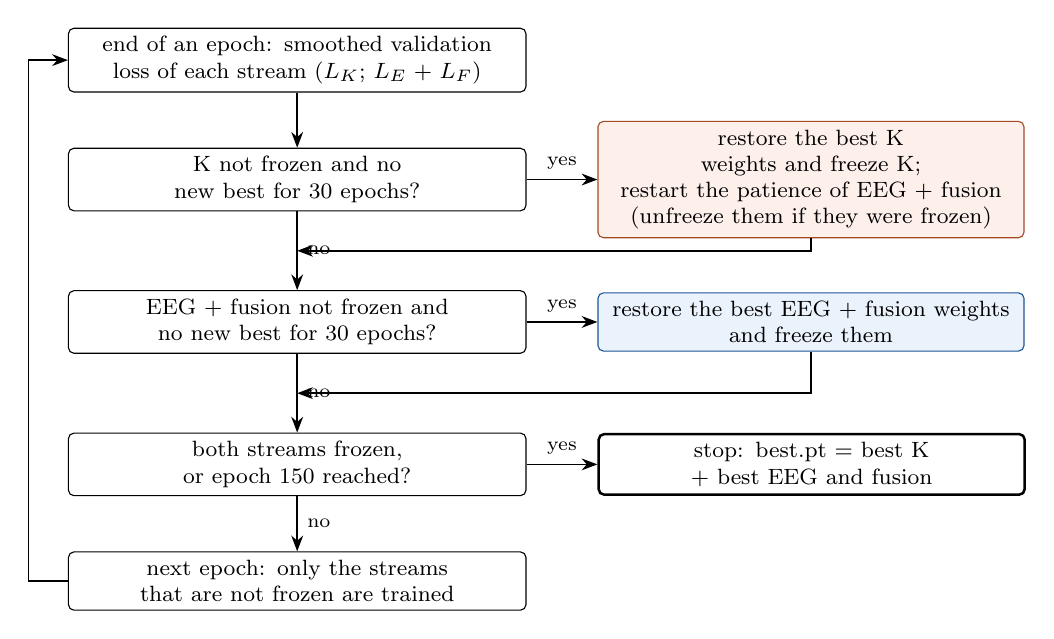
\begin{tikzpicture}[node distance=7mm and 9mm, font=\footnotesize]
\node[box, text width=5.6cm] (ep) {end of an epoch: smoothed validation loss of each stream ($L_K$; $L_E+L_F$)};
\node[box, below=of ep, text width=5.6cm] (kq) {K not frozen and no new best for 30 epochs?};
\node[kbox, right=of kq, text width=5.2cm] (kf) {restore the best K weights and freeze K;\\ restart the patience of EEG + fusion\\ (unfreeze them if they were frozen)};
\node[box, below=10mm of kq, text width=5.6cm] (eq) {EEG + fusion not frozen and no new best for 30 epochs?};
\node[ebox, right=of eq, text width=5.2cm] (ef) {restore the best EEG + fusion weights\\ and freeze them};
\node[box, below=10mm of eq, text width=5.6cm] (both) {both streams frozen, or epoch 150 reached?};
\node[result, right=of both, text width=5.2cm] (stop) {stop: best.pt = best K + best EEG and fusion};
\node[box, below=of both, text width=5.6cm] (next) {next epoch: only the streams that are not frozen are trained};
\draw[arr] (ep)--(kq);
\draw[arr] (kq)--node[lab, above]{yes}(kf);
\draw[arr] (kq)--node[lab, right]{no}(eq);
\draw[arr] (kf.south)|-($(kq.south)!0.5!(eq.north)$);
\draw[arr] (eq)--node[lab, above]{yes}(ef);
\draw[arr] (eq)--node[lab, right]{no}(both);
\draw[arr] (ef.south)|-($(eq.south)!0.5!(both.north)$);
\draw[arr] (both)--node[lab, above]{yes}(stop);
\draw[arr] (both)--node[lab, right]{no}(next);
\draw[arr] (next.west)--++(-0.5,0)|-(ep.west);
\end{tikzpicture}
\end{latin}

\caption{قاعده‌ی \lr{freezing} در پایان هر دوره. وضعیت \lr{freezing} در \lr{last.pt} ذخیره می‌شود و اگر آموزش قطع و دوباره شروع شود، حفظ می‌شود.}
\label{fig:freeze}
\end{figure}

\subsection{پیش‌بینی روی یک سری کامل}

مدل هر بار ۸ ثانیه را می‌بیند، اما یک سری چند دقیقه طول می‌کشد. برای پیش‌بینی کل سری، پنجره‌های ۸ ثانیه‌ای با فاصله‌ی ۴ ثانیه روی سری لغزانده می‌شوند و از هر پنجره فقط ۴ ثانیه‌ی وسطش نگه داشته می‌شود (شکل~\ref{fig:stitch}). دلیلش این است که \lr{tokens} نزدیک لبه‌ی پنجره بافت کمتری دارند و پیش‌بینی‌شان کم‌دقت‌تر است. اولین و آخرین پنجره لبه‌ی بیرونی‌شان را هم نگه می‌دارند تا هیچ بخشی از سری جا نماند. در آخر، \lr{tokens} ۵۰ هرتز با درون‌یابی اسپلاین مکعبی به ۵۰۰ هرتز برمی‌گردند و با پوش واقعی ۵۰۰ هرتز مقایسه می‌شوند. همین تابع در ارزیابی، تفسیر و \lr{triptych figures} به کار می‌رود.

\begin{figure}[htbp]
\centering
% Stitched inference over one series.
\begin{latin}
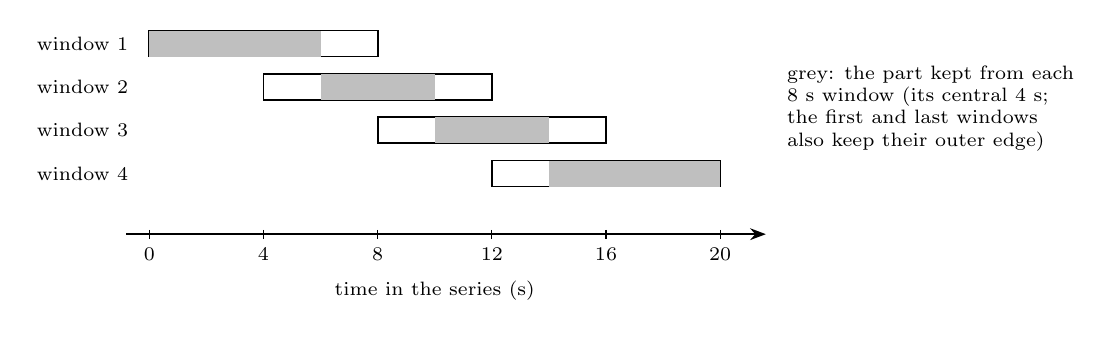
\begin{tikzpicture}[x=1.45cm, y=0.55cm, font=\footnotesize]
\foreach \i/\s in {0/0,1/4,2/8,3/12}{
  \draw[semithick] (\s/4,-\i) rectangle ++(2,0.6);
  \fill[black!25] (\s/4+0.5,-\i) rectangle ++(1,0.6);
  \node[lab, anchor=east] at (-0.1,-\i+0.3) {window \the\numexpr\i+1\relax};
}
\fill[black!25] (0,0) rectangle (0.5,0.6);
\fill[black!25] (3.5,-3) rectangle (5,-2.4);
\draw[arr] (-0.2,-4.1)--(5.4,-4.1);
\foreach \x/\t in {0/0,1/4,2/8,3/12,4/16,5/20}{\draw (\x,-4.0)--(\x,-4.2) node[lab, below]{\t};}
\node[lab] at (2.5,-5.4) {time in the series (s)};
\node[lab, anchor=west, align=left] at (5.5,-1.2) {grey: the part kept from each\\ 8 s window (its central 4 s;\\ the first and last windows\\ also keep their outer edge)};
\end{tikzpicture}
\end{latin}

\caption{پیش‌بینی پیوسته روی یک سری: پنجره‌های ۸ ثانیه‌ای با فاصله‌ی ۴ ثانیه، و نگه‌داشتن ۴ ثانیه‌ی وسط هر پنجره.}
\label{fig:stitch}
\end{figure}

\FloatBarrier
\section{نتایج ارزیابی \lr{v2}}
\label{sec:v2-results}

همه‌ی اعداد این بخش روی همان سری‌های آزمونی است که مدل پایه با آن‌ها سنجیده شد، و با نرخ ۵۰۰ هرتز. پس مقایسه‌ی دو مدل منصفانه است. آموزش هر شرکت‌کننده روی \lr{GTX 1660 Ti} بین ۱۷ تا ۳۱ دقیقه طول کشید (جدول~\ref{tab:v2-train}).

\subsection{دقت \lr{K}، \lr{E} و \lr{F}}

جدول~\ref{tab:v2-subj} خلاصه‌ی اصلی نتایج است.

\paragraph{\lr{K} از مدل پایه بهتر است.} میانگین \lr{VAF} \lr{K} \lr{۷۵٫۸} درصد و میانگین $r$ آن \lr{۰٫۸۷۲} است؛ مدل پایه \lr{۷۲٫۲} درصد و \lr{۰٫۸۵۱} داشت. این بهبود در هر ۱۲ شرکت‌کننده دیده می‌شود، نه فقط در میانگین. اندازه‌ی بهبود از \lr{۰٫۳} واحد (\lr{P5}) تا \lr{۵٫۵} واحد (\lr{P4}) است و میانه‌اش حدود ۴ واحد. \lr{K} حتی از مدل فقط‌سینماتیکِ \lr{residual experiment} (\lr{۷۵٫۵} درصد و \lr{۰٫۸۶۹}) هم کمی بهتر است. پس اولین معیار پذیرش \lr{v2} برآورده شد.

\begin{table}[htbp]
\centering
\small
\caption{نتایج \lr{v2} روی سری‌های آزمون در برابر مدل پایه. چهار ستون اول \lr{VAF} (درصد) و چهار ستون بعد \lr{r}، هر دو میانگین روی پنج عضله.}
\label{tab:v2-subj}
\begin{tabular}{lcccccccc}
\toprule
شرکت‌کننده & پایه & \lr{K} & \lr{E} & \lr{F} & پایه & \lr{K} & \lr{E} & \lr{F} \\
\midrule
\lr{P1} & \lr{۷۹٫۰} & \lr{۸۳٫۶} & \lr{۳۳٫۹} & \lr{۸۳٫۸} & \lr{۰٫۸۹۱} & \lr{۰٫۹۱۴} & \lr{۰٫۵۹۷} & \lr{۰٫۹۱۵} \\
\lr{P2} & \lr{۷۵٫۲} & \lr{۷۸٫۸} & \lr{۵۸٫۳} & \lr{۷۸٫۸} & \lr{۰٫۸۷۲} & \lr{۰٫۸۸۸} & \lr{۰٫۷۶۶} & \lr{۰٫۸۸۸} \\
\lr{P3} & \lr{۶۷٫۵} & \lr{۶۹٫۸} & \lr{۳۰٫۷} & \lr{۷۰٫۲} & \lr{۰٫۸۱۱} & \lr{۰٫۸۳۷} & \lr{۰٫۵۹۲} & \lr{۰٫۸۳۶} \\
\lr{P4} & \lr{۷۶٫۰} & \lr{۸۱٫۵} & \lr{۵۷٫۷} & \lr{۸۱٫۸} & \lr{۰٫۸۸۰} & \lr{۰٫۹۰۵} & \lr{۰٫۷۵۹} & \lr{۰٫۹۰۵} \\
\lr{P5} & \lr{۶۳٫۵} & \lr{۶۳٫۸} & \lr{۳۴٫۴} & \lr{۶۴٫۰} & \lr{۰٫۷۷۷} & \lr{۰٫۷۹۵} & \lr{۰٫۶۰۳} & \lr{۰٫۷۹۳} \\
\lr{P6} & \lr{۷۴٫۷} & \lr{۷۶٫۷} & \lr{۳۵٫۸} & \lr{۷۷٫۰} & \lr{۰٫۸۶۵} & \lr{۰٫۸۷۷} & \lr{۰٫۶۲۶} & \lr{۰٫۸۷۷} \\
\lr{P7} & \lr{۷۹٫۱} & \lr{۸۲٫۶} & \lr{۵۷٫۷} & \lr{۸۲٫۵} & \lr{۰٫۸۹۹} & \lr{۰٫۹۱۰} & \lr{۰٫۷۵۶} & \lr{۰٫۹۱۱} \\
\lr{P8} & \lr{۵۴٫۳} & \lr{۵۸٫۴} & \lr{۳۲٫۷} & \lr{۵۸٫۰} & \lr{۰٫۷۶۴} & \lr{۰٫۷۹۲} & \lr{۰٫۵۸۲} & \lr{۰٫۷۹۹} \\
\lr{P9} & \lr{۷۹٫۳} & \lr{۸۳٫۵} & \lr{۴٫۵} & \lr{۸۳٫۵} & \lr{۰٫۸۹۷} & \lr{۰٫۹۱۸} & \lr{۰٫۴۷۸} & \lr{۰٫۹۱۸} \\
\lr{P10} & \lr{۷۴٫۹} & \lr{۸۰٫۲} & \lr{۵۳٫۶} & \lr{۸۰٫۳} & \lr{۰٫۸۷۱} & \lr{۰٫۸۹۸} & \lr{۰٫۷۲۵} & \lr{۰٫۸۹۸} \\
\lr{P11} & \lr{۷۳٫۶} & \lr{۷۸٫۱} & \lr{۳۶٫۰} & \lr{۷۸٫۱} & \lr{۰٫۸۵۸} & \lr{۰٫۸۸۴} & \lr{۰٫۶۴۹} & \lr{۰٫۸۸۴} \\
\lr{P12} & \lr{۶۹٫۸} & \lr{۷۲٫۵} & \lr{۳۴٫۴} & \lr{۷۲٫۳} & \lr{۰٫۸۳۲} & \lr{۰٫۸۴۵} & \lr{۰٫۶۰۴} & \lr{۰٫۸۴۵} \\
\midrule
\textbf{میانگین} & \lr{۷۲٫۲} & \lr{۷۵٫۸} & \lr{۳۹٫۱} & \lr{۷۵٫۹} & \lr{۰٫۸۵۱} & \lr{۰٫۸۷۲} & \lr{۰٫۶۴۵} & \lr{۰٫۸۷۲} \\
\bottomrule
\end{tabular}
\end{table}


\paragraph{\lr{E} از \lr{EEG} به‌تنهایی پیش‌بینی معناداری می‌سازد.} \lr{E} که فقط \lr{EEG} می‌بیند به $r$ \lr{۰٫۶۴۵} و \lr{VAF} \lr{۳۹٫۱} درصد رسید. این از خروجی فقط‌\lr{EEG} آزمایش‌های قبلی ($r$ حدود \lr{۰٫۴۷}) بالاتر است.

آیا ممکن است این عدد تصادفی باشد؟ برای پاسخ، \lr{null test} انجام شد: بلوک‌های \lr{EEG} در زمان جابه‌جا می‌شوند تا رابطه‌اش با حرکت از بین برود، و دقت دوباره حساب می‌شود. \lr{E} واقعی در هر ۱۲ شرکت‌کننده از این حالت جابه‌جاشده بهتر بود (جدول~\ref{tab:v2-verdict}). پس \lr{EEG} به‌تنهایی اطلاعات واقعی درباره‌ی حرکت دارد.

\paragraph{\lr{F} همان \lr{K} است.} میانگین \lr{VAF} \lr{F} \lr{۷۵٫۹} و \lr{K} \lr{۷۵٫۸} است. بزرگ‌ترین قدرمطلق \lr{gate} در هر شرکت‌کننده بین \lr{۰٫۰۱} و \lr{۰٫۰۴} ماند، و اصلاحی که \lr{EEG} اضافه می‌کند حدود \lr{۰٫۲} تا ۲ درصد اندازه‌ی \lr{K} است (جدول~\ref{tab:interp-parts}). فقط در یک نفر (\lr{P4}) بهتر بودن \lr{F} نسبت به \lr{K} از \lr{null test} گذشت؛ از ۱۲ آزمون، یک نتیجه‌ی معنادار همان چیزی است که از شانس انتظار می‌رود.

این یعنی \lr{EEG} چیزی به سینماتیک اضافه نمی‌کند. ولی شاید مشکل از ماژول \lr{fusion} باشد که نتوانسته اطلاعات موجود را یاد بگیرد. بخش~\ref{sec:residual} این احتمال را جداگانه بررسی می‌کند و نشان می‌دهد این‌طور نیست.

\begin{table}[htbp]
\centering
\small
\caption{\lr{null tests}: \lr{E} در برابر \lr{EEG} جابه‌جاشده بین بلوک‌ها، و بهره‌ی \lr{F} نسبت به \lr{K}. \lr{p} هیچ‌گاه کمتر از یک‌تقسیم‌بر‌تعداد بلوک‌ها گزارش نمی‌شود. ستون آخر بزرگ‌ترین قدرمطلق \lr{gate} \lr{fusion} بین پنج عضله است.}
\label{tab:v2-verdict}
\begin{tabular}{cccccc}
\toprule
شرکت‌کننده & \lr{r} خروجی \lr{E} & \lr{p} (جابه‌جایی) & $\Delta$\lr{VAF} (\lr{F}$-$\lr{K}) & \lr{p} (جابه‌جایی) & بیشینه‌ی $|g|$ \\
\midrule
\lr{P1} & \lr{۰٫۵۹۷} & \lr{۰٫۰۱۲} & \lr{+۰٫۱۹} & \lr{۰٫۱۹} & \lr{۰٫۰۱۵} \\
\lr{P2} & \lr{۰٫۷۶۶} & \lr{۰٫۰۱۱} & \lr{−۰٫۰۲} & \lr{۰٫۸۵} & \lr{۰٫۰۱۴} \\
\lr{P3} & \lr{۰٫۵۹۲} & \lr{۰٫۰۱۳} & \lr{+۰٫۳۷} & \lr{۰٫۹۵} & \lr{۰٫۰۱۷} \\
\lr{P4} & \lr{۰٫۷۵۹} & \lr{۰٫۰۱۲} & \lr{+۰٫۳۲} & \lr{۰٫۰۱} & \lr{۰٫۰۲۶} \\
\lr{P5} & \lr{۰٫۶۰۳} & \lr{۰٫۰۱۱} & \lr{+۰٫۲۵} & \lr{۰٫۱۸} & \lr{۰٫۰۲۶} \\
\lr{P6} & \lr{۰٫۶۲۶} & \lr{۰٫۰۱۱} & \lr{+۰٫۳۵} & \lr{۰٫۲۶} & \lr{۰٫۰۲۴} \\
\lr{P7} & \lr{۰٫۷۵۶} & \lr{۰٫۰۱۱} & \lr{−۰٫۰۲} & \lr{۰٫۷۸} & \lr{۰٫۰۱۸} \\
\lr{P8} & \lr{۰٫۵۸۲} & \lr{۰٫۰۱۳} & \lr{−۰٫۳۵} & \lr{۰٫۳۴} & \lr{۰٫۰۴۲} \\
\lr{P9} & \lr{۰٫۴۷۸} & \lr{۰٫۰۱۲} & \lr{+۰٫۰۳} & \lr{۰٫۳۴} & \lr{۰٫۰۱۲} \\
\lr{P10} & \lr{۰٫۷۲۵} & \lr{۰٫۰۱۲} & \lr{+۰٫۰۶} & \lr{۰٫۴۰} & \lr{۰٫۰۱۰} \\
\lr{P11} & \lr{۰٫۶۴۹} & \lr{۰٫۰۱۱} & \lr{+۰٫۰۱} & \lr{۰٫۴۵} & \lr{۰٫۰۱۵} \\
\lr{P12} & \lr{۰٫۶۰۴} & \lr{۰٫۰۱۰} & \lr{−۰٫۲۲} & \lr{۰٫۸۲} & \lr{۰٫۰۲۱} \\
\bottomrule
\end{tabular}
\end{table}


\paragraph{کی می‌توان به \lr{F} اعتماد کرد.} \lr{F} روی \lr{K} ساخته می‌شود، پس \lr{fusion} ذخیره‌شده فقط وقتی معنا دارد که با همان \lr{K} ذخیره‌شده آموزش دیده باشد. دفترچه‌ی آموزش این شرط را بررسی می‌کند. با قاعده‌ی \lr{freezing}، بهترین دوره‌ی \lr{EEG} و \lr{fusion} همیشه بعد از \lr{freeze} شدن \lr{K} است (جدول~\ref{tab:v2-train})، پس شرط در هر ۱۲ نفر برقرار است.

جدول حکم‌هایی که این گزارش از آن استفاده می‌کند پیش از اصلاح این بررسی ذخیره شده است. به همین دلیل برای ۹ نفر برچسب «غیرقابل‌تفسیر» دارد. اعداد جدول درست‌اند؛ اگر سلول ارزیابی دوباره اجرا شود، این برچسب‌ها به «\lr{EEG} چیزی به سینماتیک اضافه نمی‌کند» تغییر می‌کنند (به‌جز \lr{P4}).

\begin{table}[htbp]
\centering
\small
\caption{روند آموزش \lr{v2}: شماره‌ی بهترین دوره و دوره‌ی \lr{freezing} هر جریان. خط تیره یعنی جریان تا پایان (۱۵۰ دوره) منجمد نشد.}
\label{tab:v2-train}
\begin{tabular}{ccccccc}
\toprule
شرکت‌کننده & دوره‌ها & بهترین \lr{K} & \lr{freezing} \lr{K} & بهترین \lr{E} & \lr{freezing} \lr{E} & زمان (دقیقه) \\
\midrule
\lr{P1} & \lr{۱۵۰} & \lr{۸۰} & \lr{۱۱۰} & \lr{۱۲۷} & -- & \lr{۲۴٫۱} \\
\lr{P2} & \lr{۱۵۰} & \lr{۱۱۶} & \lr{۱۴۶} & \lr{۱۴۷} & -- & \lr{۳۰٫۸} \\
\lr{P3} & \lr{۱۰۵} & \lr{۳۱} & \lr{۶۱} & \lr{۷۵} & \lr{۱۰۵} & \lr{۱۷٫۲} \\
\lr{P4} & \lr{۱۳۸} & \lr{۵۵} & \lr{۸۵} & \lr{۱۰۸} & \lr{۱۳۸} & \lr{۲۳٫۹} \\
\lr{P5} & \lr{۱۵۰} & \lr{۵۵} & \lr{۸۵} & \lr{۱۲۵} & -- & \lr{۲۷٫۹} \\
\lr{P6} & \lr{۱۲۲} & \lr{۴۹} & \lr{۷۹} & \lr{۹۲} & \lr{۱۲۲} & \lr{۲۳٫۱} \\
\lr{P7} & \lr{۱۰۵} & \lr{۳۸} & \lr{۶۸} & \lr{۷۵} & \lr{۱۰۵} & \lr{۲۱٫۹} \\
\lr{P8} & \lr{۱۳۸} & \lr{۲۷} & \lr{۵۷} & \lr{۱۰۸} & \lr{۱۳۸} & \lr{۲۲٫۹} \\
\lr{P9} & \lr{۱۵۰} & \lr{۷۳} & \lr{۱۰۳} & \lr{۱۲۰} & \lr{۱۵۰} & \lr{۲۴٫۶} \\
\lr{P10} & \lr{۱۱۰} & \lr{۴۹} & \lr{۷۹} & \lr{۸۰} & \lr{۱۱۰} & \lr{۱۹٫۳} \\
\lr{P11} & \lr{۹۵} & \lr{۳۳} & \lr{۶۳} & \lr{۶۵} & \lr{۹۵} & \lr{۱۷٫۸} \\
\lr{P12} & \lr{۹۰} & \lr{۱۹} & \lr{۴۹} & \lr{۶۰} & \lr{۹۰} & \lr{۱۷٫۳} \\
\bottomrule
\end{tabular}
\end{table}


\fig{v2_history_P1.png}{0.85}{خطای \lr{validation} \lr{P1} در طول آموزش: چپ \lr{K}، راست \lr{E}+\lr{F}. \lr{K} در دوره‌ی ۸۰ بهترین بود و در دوره‌ی ۱۱۰ \lr{freeze} شد؛ \lr{EEG} و \lr{fusion} تا دوره‌ی ۱۵۰ ادامه دادند.}

\subsection{هر عضله و سقف داده}

جدول~\ref{tab:v2-musc} نشان می‌دهد \lr{K} در همه‌ی پنج عضله از مدل پایه بهتر است.

ستون «سقف» جدول می‌گوید در بهترین حالت چه عددی ممکن است. این عدد \lr{VAF} خود پوش واقعی پس از صاف کردن با \lr{low-pass} ۲ هرتز است؛ یعنی دقت یک پیش‌بین هموار که همه‌چیز را درست می‌داند و فقط نوسان‌های سریع را نمی‌تواند بسازد. \lr{FD} محدودترین عضله است: سقفش ۷۴ درصد است و فعالیتش تغییر کمی دارد (\lr{modulation depth} کم: صدک ۸۰ فقط حدود دو برابر صدک ۲۰ است). برای \lr{AD}، \lr{BR} و \lr{ED} فاصله‌ی \lr{K} تا سقف حدود ۸ تا ۱۱ واحد است؛ یعنی هنوز جا برای بهتر شدن هست.

\begin{table}[htbp]
\centering
\small
\caption{\lr{VAF} (درصد) برای هر عضله، میانگین روی ۱۲ شرکت‌کننده؛ \lr{smooth ceiling} = \lr{VAF} خودِ هدفِ هموارشده با \lr{low-pass} ۲ هرتز؛ \lr{modulation depth} = نسبت صدک ۸۰ به صدک ۲۰ هدف.}
\label{tab:v2-musc}
\begin{tabular}{ccccccc}
\toprule
عضله & پایه & \lr{K} & \lr{E} & \lr{F} & \lr{smooth ceiling} & \lr{modulation depth} \\
\midrule
\lr{AD} & \lr{۸۵٫۹} & \lr{۸۸٫۶} & \lr{۵۸٫۰} & \lr{۸۸٫۷} & \lr{۹۳٫۷} & \lr{۱۲٫۲} \\
\lr{BR} & \lr{۷۹٫۶} & \lr{۸۲٫۵} & \lr{۴۴٫۴} & \lr{۸۲٫۹} & \lr{۹۰٫۵} & \lr{۳٫۲} \\
\lr{FD} & \lr{۴۹٫۵} & \lr{۵۳٫۰} & \lr{۱۸٫۱} & \lr{۵۲٫۷} & \lr{۷۴٫۲} & \lr{۲٫۰} \\
\lr{ED} & \lr{۸۲٫۴} & \lr{۸۶٫۱} & \lr{۵۲٫۴} & \lr{۸۶٫۴} & \lr{۹۳٫۳} & \lr{۵٫۰} \\
\lr{FDI} & \lr{۶۳٫۷} & \lr{۶۸٫۶} & \lr{۲۲٫۷} & \lr{۶۸٫۵} & \lr{۸۷٫۱} & \lr{۳٫۵} \\
\bottomrule
\end{tabular}
\end{table}


\subsection{دامنه در هر وزن جسم}

یکی از کاستی‌های مدل پایه این بود که خطای دامنه به وزن جسم بستگی داشت. جدول~\ref{tab:v2-load} این را برای سه وزن مقایسه می‌کند. دو چیز سنجیده شده است: \lr{height ratio} در زمان نگه‌داشتن، و همبستگی سطح فعالیت بین بلندکردن‌هایی که وزن یکسان دارند.

جزء \lr{lift} در \lr{loss function} و ویژگی‌های تاریخچه دقیقاً برای همین خطا طراحی شدند و اثرشان روشن است. مدل پایه وزن سبک را \lr{۴٫۵} درصد و وزن متوسط را \lr{۵٫۵} درصد بیش‌برآورد می‌کرد. \lr{height ratio} \lr{K} در هر سه وزن بین \lr{۱٫۰۰۴} و \lr{۱٫۰۰۹} است، یعنی خطای کمتر از یک درصد. معیار پذیرش دوم این بود که این عدد بین \lr{۰٫۹۵} و \lr{۱٫۰۵} باشد.

همبستگی سطح فعالیت بین بلندکردن‌های هم‌وزن هم در هر سه وزن بالا رفته است؛ مثلاً در وزن سبک از \lr{۰٫۳۹} به \lr{۰٫۵۳}. یعنی \lr{K} بهتر از مدل پایه تشخیص می‌دهد کدام بلندکردن کمی بیشتر یا کمتر از بقیه زور می‌خواهد.

\begin{table}[htbp]
\centering
\small
\caption{سطح فعالیت در مرحله‌ی نگه‌داشتن، برای هر وزن جسم (میانگین روی شرکت‌کننده‌ها، سری‌ها و عضله‌ها). \lr{height ratio} = میانگین پیش‌بینی به میانگین هدف؛ مقدار مطلوب ۱.}
\label{tab:v2-load}
\begin{tabular}{ccccc}
\toprule
وزن جسم & \lr{height ratio} پایه & \lr{height ratio} \lr{K} & \lr{r} بین بلندکردن‌ها پایه & \lr{r} بین بلندکردن‌ها \lr{K} \\
\midrule
سبک & \lr{۱٫۰۴۵} & \lr{۱٫۰۰۵} & \lr{۰٫۳۹۱} & \lr{۰٫۵۲۹} \\
متوسط & \lr{۱٫۰۵۵} & \lr{۱٫۰۰۴} & \lr{۰٫۵۰۱} & \lr{۰٫۵۷۰} \\
سنگین & \lr{۱٫۰۲۴} & \lr{۱٫۰۰۹} & \lr{۰٫۳۹۴} & \lr{۰٫۴۶۱} \\
\bottomrule
\end{tabular}
\end{table}


\subsection{\lr{triptych figures}}

برای اینکه ببینیم مدل در عمل چه می‌کند، هر سری آزمون به تکه‌های ۱۰ ثانیه‌ای تقسیم و برای هر تکه یک شکل سه‌پنلی (\lr{triptych}) ساخته شد. در ادامه برای شرکت‌کننده‌های ۱ تا ۴ و برای هر سری آزمون یک شکل آمده است (ثانیه‌ی ۳۰ تا ۴۰ هر سری).

\begin{itemize}
\item \textbf{پنل ۱: پیش‌بینی در برابر واقعیت.} پوش واقعی (سیاه) کنار \lr{K} (نارنجی)، \lr{E} (آبی) و \lr{F} (سبز خط‌چین)، با واحد اصلی. خطوط عمودی رخدادهای آزمایش‌اند: روشن شدن چراغ، اولین تماس، جدا شدن جسم از سطح، گذاشتن و رها کردن. ناحیه‌ی زرد بازه‌ی نگه‌داشتن است. ستون راست $r$ همین تکه را می‌دهد.
\item \textbf{پنل ۲: اجزای خروجی.} $K_{base}$ (خاکستری)، $K=K_{base}\cdot g$ (نارنجی) و اصلاح \lr{EEG}، $F_{eeg}$ (بنفش)، در حوزه‌ی جذر. ستون راست بازه‌ی ضریب تاریخچه و نسبت اندازه‌ی اصلاح \lr{EEG} به \lr{K} را می‌دهد.
\item \textbf{پنل ۳: توجه بین عضله‌ها.} \lr{attention rollout} \lr{muscle graph} جریان سینماتیک، به‌صورت تغییر نسبت به میانگین استراحت همان سری. هر بلوک یک عضله‌ی گیرنده و هر سطر یک عضله‌ی فرستنده است.
\end{itemize}

الگوی همه‌ی شکل‌ها یکی است. \lr{F} دقیقاً روی \lr{K} افتاده و $F_{eeg}$ نزدیک صفر است. \lr{E} زمان‌بندی کلی هر بلندکردن را درست دنبال می‌کند، اما جهش‌های کوتاه و تیز پوش را ندارد.

\fig{trip_P1_S04.png}{0.82}{\lr{P1}، سری آزمون ۴، ثانیه‌ی ۳۰ تا ۴۰.}
\fig{trip_P1_S05.png}{0.82}{\lr{P1}، سری آزمون ۵، ثانیه‌ی ۳۰ تا ۴۰.}
\fig{trip_P2_S05.png}{0.82}{\lr{P2}، سری آزمون ۵، ثانیه‌ی ۳۰ تا ۴۰.}
\fig{trip_P2_S06.png}{0.82}{\lr{P2}، سری آزمون ۶، ثانیه‌ی ۳۰ تا ۴۰.}
\fig{trip_P3_S04.png}{0.82}{\lr{P3}، سری آزمون ۴، ثانیه‌ی ۳۰ تا ۴۰.}
\fig{trip_P3_S06.png}{0.82}{\lr{P3}، سری آزمون ۶، ثانیه‌ی ۳۰ تا ۴۰.}
\fig{trip_P4_S04.png}{0.82}{\lr{P4}، سری آزمون ۴، ثانیه‌ی ۳۰ تا ۴۰.}
\fig{trip_P4_S05.png}{0.82}{\lr{P4}، سری آزمون ۵، ثانیه‌ی ۳۰ تا ۴۰.}
\clearpage

\FloatBarrier
\section{تفسیرپذیری در \lr{v2}}
\label{sec:interp}

دقت به ما می‌گوید مدل چقدر خوب پیش‌بینی می‌کند. تفسیرپذیری می‌پرسد مدل برای این پیش‌بینی به کدام ورودی‌ها تکیه کرده است: کدام لحظه‌ها، کدام الکترودها، کدام باندها و کدام عضله‌ها. این بخش روش‌ها را توضیح می‌دهد، نشان می‌دهد چطور خودِ روش‌ها سنجیده شدند و نتایج را برای همه‌ی شرکت‌کننده‌ها و با جزئیات برای \lr{P1} و \lr{P2} می‌آورد.

\subsection{چه چیزی توضیح داده می‌شود}

هر توضیح درباره‌ی یک عدد مشخص است: خروجی $o$ (یکی از $K$، $E$ یا $F_{eeg}$)، برای عضله‌ی $c$، در \lr{token} $t$ از یک پنجره‌ی ۸ ثانیه‌ای:
\begin{equation}
y=\mathrm{out}_o[t,c].
\end{equation}
پنجره‌ها دور رخدادهای مهم آزمایش ساخته می‌شوند: «اولین تماس» (انگشت به جسم می‌رسد) و «جدا شدن» (\lr{lift-off}، جسم از سطح بلند می‌شود). $t$ وسط پنجره است، یعنی خودِ لحظه‌ی رخداد. پس پرسش این است: «مدل برای پیش‌بینی فعالیت عضله در لحظه‌ی رخداد، به کجای ورودی نگاه کرده است؟»

مسیری که هر خروجی از ورودی طی می‌کند:
\begin{itemize}
\item $K$: \lr{stem}، سه لایه‌ی زمانی سینماتیک، دو لایه‌ی \lr{muscle graph}؛
\item $E$: دو لایه‌ی \lr{electrode graph}، \lr{attention pooling}، دو لایه‌ی زمانی \lr{EEG}، دو لایه‌ی \lr{muscle graph}؛
\item $F_{eeg}$: \lr{electrode graph}، \lr{attention pooling}، لایه‌های زمانی \lr{EEG} و \lr{cross-attention}.
\end{itemize}
\lr{recorder} در یک بار اجرای مدل، ماتریس توجه همه‌ی این لایه‌ها را برمی‌دارد: $A^{h}_{l}\in\mathbb{R}^{n\times n}$ برای لایه‌ی $l$ و سر $h$. همه‌ی روش‌های زیر از همین ماتریس‌ها یا از گرادیان $y$ نسبت به آن‌ها ساخته می‌شوند. شکل~\ref{fig:interp-pipeline} کل فرایند را نشان می‌دهد.

\begin{figure}[htbp]
\centering
% Interpretability pipeline of v2.
\begin{latin}
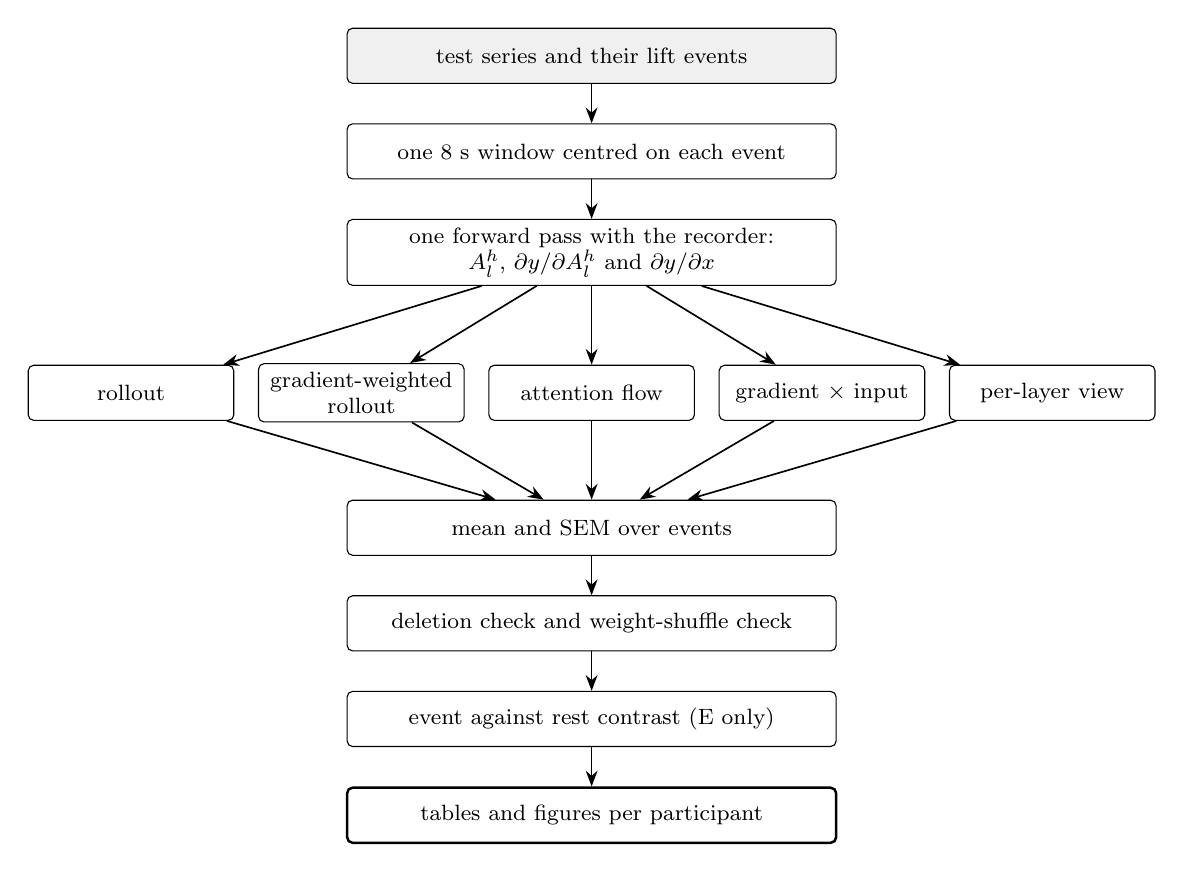
\begin{tikzpicture}[node distance=5mm and 3mm, font=\footnotesize]
\node[io, text width=6cm] (ev) {test series and their lift events};
\node[box, below=of ev, text width=6cm] (win) {one 8 s window centred on each event};
\node[box, below=of win, text width=6cm] (rec) {one forward pass with the recorder:\\ $A^{h}_{l}$, $\partial y/\partial A^{h}_{l}$ and $\partial y/\partial x$};
\node[box, below=10mm of rec, text width=2.4cm] (v3) {attention flow};
\node[box, left=of v3, text width=2.4cm] (v2) {gradient-weighted rollout};
\node[box, left=of v2, text width=2.4cm] (v1) {rollout};
\node[box, right=of v3, text width=2.4cm] (v4) {gradient $\times$ input};
\node[box, right=of v4, text width=2.4cm] (v5) {per-layer view};
\node[box, below=10mm of v3, text width=6cm] (avg) {mean and SEM over events};
\node[box, below=of avg, text width=6cm] (chk) {deletion check and weight-shuffle check};
\node[box, below=of chk, text width=6cm] (con) {event against rest contrast (E only)};
\node[result, below=of con, text width=6cm] (out) {tables and figures per participant};
\draw[arr] (ev)--(win); \draw[arr] (win)--(rec);
\foreach \v in {v1,v2,v3,v4,v5}{\draw[arr] (rec)--(\v); \draw[arr] (\v)--(avg);}
\draw[arr] (avg)--(chk); \draw[arr] (chk)--(con); \draw[arr] (con)--(out);
\end{tikzpicture}
\end{latin}

\caption{فرایند تفسیر در \lr{v2}: هر روش از یک اجرای ثبت‌شده ساخته می‌شود، روی رخدادها میانگین گرفته می‌شود و پیش از هر ادعا، خود روش سنجیده می‌شود.}
\label{fig:interp-pipeline}
\end{figure}

\subsection{\lr{attention rollout} و \lr{attention flow}}

این دو روش توجه همه‌ی لایه‌ها را پشت سر هم ترکیب می‌کنند تا از خروجی به ورودی برسند. چون پایه‌ی بیشتر نتایج این گزارش‌اند، بخش جداگانه‌ی~\ref{sec:rollout-flow} آن‌ها را با جزئیات توضیح می‌دهد. برای این بخش همین کافی است: \lr{rollout} در هر لایه ماتریس $\hat A_l=\tfrac12\overline{A}_l+\tfrac12 I$ را می‌سازد (میانگین سرها، به‌علاوه‌ی راه مستقیم \lr{residual connection}) و این ماتریس‌ها را در هم ضرب می‌کند: $R=\hat A_L\cdots\hat A_1$. نتیجه برای هر \lr{token} ورودی یک سهم بین ۰ و ۱ است و جمع سهم‌ها ۱ می‌شود. این سهم برای هر پنج عضله‌ی یک جریان یکسان است، چون توجه زمانی بین عضله‌ها مشترک است.

\subsection{\lr{gradient-weighted rollout}}

\textbf{ایده.} \lr{plain rollout} همه‌ی توجه‌ها را به یک اندازه مهم می‌داند. اما ممکن است یک سر توجه، اطلاعاتی را جابه‌جا کند که برای عضله‌ی موردنظر اصلاً اهمیتی ندارد. \lr{gradient-weighted rollout} \cite{chefer2021} این را اصلاح می‌کند: هر وزن توجه در گرادیان خروجی نسبت به همان وزن ضرب می‌شود. گرادیان می‌گوید اگر این وزن کمی بیشتر شود، خروجی چقدر و در کدام جهت تغییر می‌کند. فقط بخش مثبت نگه داشته می‌شود، یعنی توجه‌هایی که خروجی را بالا می‌برند. چون گرادیان برای هر عضله فرق می‌کند، نقشه هم برای هر عضله جداست.

\textbf{ریاضی.}
\begin{equation}
G_l=\frac1H\sum_h\Big(A^{h}_l\odot\frac{\partial y}{\partial A^{h}_l}\Big)^{+},\qquad
\tilde A_l=\frac{G_l}{G_l\mathbf 1},\qquad
R^{\nabla}=\prod_{l=L}^{1}\Big(\tfrac12\tilde A_l+\tfrac12 I\Big).
\end{equation}
$(\cdot)^{+}$ مقادیر منفی را صفر می‌کند. تقسیم بر $G_l\mathbf 1$ هر سطر را دوباره به جمع ۱ می‌رساند؛ سطری که همه‌اش صفر شده همان $I$ می‌ماند. بقیه‌ی کار دقیقاً مثل \lr{rollout} است. گرادیان‌ها با \lr{recorder} در حالت \lr{grad=True} گرفته می‌شوند.

\begin{figure}[htbp]
\centering
% Gradient-weighted rollout.
\begin{latin}
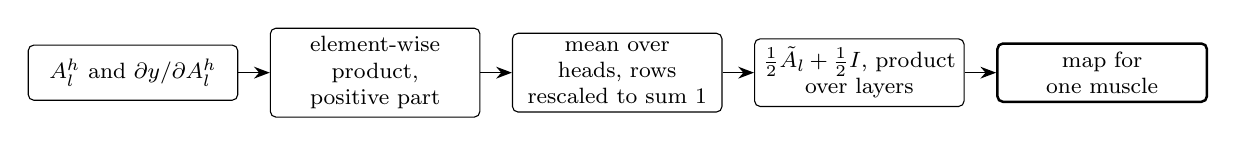
\begin{tikzpicture}[node distance=4mm and 4mm, font=\footnotesize, box/.append style={text width=2.45cm}]
\node[box] (a) {$A^{h}_l$ and $\partial y/\partial A^{h}_l$};
\node[box, right=of a] (b) {element-wise product, positive part};
\node[box, right=of b] (c) {mean over heads, rows rescaled to sum 1};
\node[box, right=of c] (d) {$\tfrac12\tilde A_l+\tfrac12I$, product over layers};
\node[result, right=of d] (e) {map for one muscle};
\draw[arr] (a)--(b); \draw[arr] (b)--(c); \draw[arr] (c)--(d); \draw[arr] (d)--(e);
\end{tikzpicture}
\end{latin}

\caption{\lr{gradient-weighted rollout}.}
\end{figure}

\subsection{نمای هر لایه}

\lr{rollout} لایه‌ها را با هم ترکیب می‌کند و نمی‌گوید کدام لایه چه کرده است. نمای هر لایه همین را نشان می‌دهد: توجه هر لایه و هر سر در لحظه‌ی رخداد، بدون ترکیب. برای لایه‌های زمانی سطر $t$ از $A^{h}_l$، و برای \lr{electrode graph} و \lr{muscle graph} کل ماتریس رسم می‌شود.

\subsection{\lr{gradient × input}}

\textbf{ایده.} \lr{rollout} فقط لایه‌های توجه را می‌بیند. لایه‌هایی مثل \lr{embedding}، \lr{feed-forward} و \lr{decoder} در آن غایب‌اند، و \lr{rollout} نمی‌تواند بگوید کدام ویژگی ورودی (مثلاً کدام باند \lr{EEG}) مهم بوده است. \lr{gradient × input} \cite{shrikumar2016} از کل مدل استفاده می‌کند: مقدار هر ورودی را در گرادیان خروجی نسبت به آن ضرب می‌کند. نتیجه تقریباً می‌گوید اگر این ورودی صفر شود، خروجی چقدر تغییر می‌کند.

\textbf{ریاضی.} برای ورودی $x$ (سینماتیک، تاریخچه یا \lr{band power} \lr{EEG}):
\begin{equation}
s_i=\Big|x_i\,\frac{\partial y}{\partial x_i}\Big|.
\end{equation}
برای هر ویژگی سینماتیک، $s$ روی زمان جمع زده می‌شود. برای هر باند \lr{EEG}، روی زمان و همه‌ی الکترودها. سپس عددها به سهم (با جمع ۱) تبدیل می‌شوند.

\begin{figure}[htbp]
\centering
% Gradient x input.
\begin{latin}
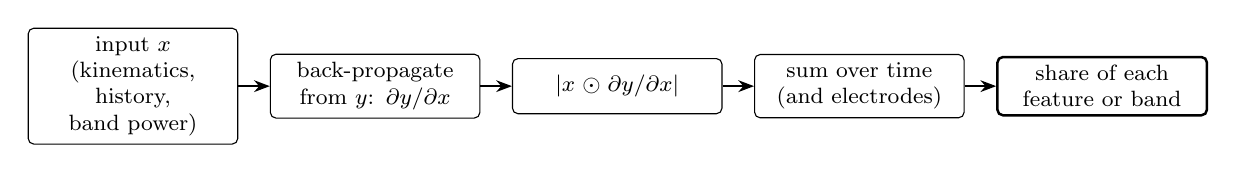
\begin{tikzpicture}[node distance=4mm and 4mm, font=\footnotesize, box/.append style={text width=2.45cm}]
\node[box] (a) {input $x$ (kinematics, history, band power)};
\node[box, right=of a] (b) {back-propagate from $y$: $\partial y/\partial x$};
\node[box, right=of b] (c) {$|x\odot\partial y/\partial x|$};
\node[box, right=of c] (d) {sum over time (and electrodes)};
\node[result, right=of d] (e) {share of each feature or band};
\draw[arr] (a)--(b); \draw[arr] (b)--(c); \draw[arr] (c)--(d); \draw[arr] (d)--(e);
\end{tikzpicture}
\end{latin}

\caption{\lr{gradient × input}.}
\end{figure}

\subsection{میانگین روی رخدادها و مقایسه با استراحت}

\textbf{میانگین روی رخدادها.} نقشه‌ی یک پنجره‌ی تنها پرنویز است، پس هیچ نقشه‌ای از یک پنجره گزارش نمی‌شود. برای هر رخداد یک پنجره ساخته می‌شود، نقشه‌اش به سهم (جمع ۱) تبدیل می‌شود و سپس میانگین و خطای استاندارد ($\mathrm{SEM}=\sigma/\sqrt n$) روی همه‌ی رخدادها گرفته می‌شود. رخدادی که پنجره‌ی ۸ ثانیه‌ای‌اش در سری جا نشود کنار گذاشته می‌شود.

\textbf{مقایسه با استراحت (فقط برای \lr{E}).} حتی اگر یک الکترود سهم بالایی داشته باشد، شاید همیشه سهم بالایی داشته باشد و ربطی به حرکت نداشته باشد. برای جدا کردن این دو، هر بلندکردن با یک پنجره‌ی استراحت بعد از آن (وسط فاصله‌ی دو بلندکردن) جفت می‌شود. برای هر الکترود $e$ تفاوت سهم در رخداد و استراحت ($d_{ie}=a_{ie}-b_{ie}$) و آماره‌ی $t_e=\bar d_e/(s_e/\sqrt n)$ حساب می‌شود. $t$ بزرگ یعنی این الکترود در رخداد به‌طور پایدار سهم بیشتری دارد تا در استراحت.

برای $p$، علامت تفاوت هر جفت ۱۰۰۰ بار به‌طور تصادفی برگردانده می‌شود. هر بار بزرگ‌ترین $|t|$ روی همه‌ی ۳۲ الکترود نگه داشته می‌شود و $p$ هر الکترود از مقایسه با این بیشینه‌ها به دست می‌آید (\lr{max-T}، \cite{nichols2002}). این کار دو مزیت دارد. اول، خطای ناشی از آزمودن ۳۲ الکترود با هم را کنترل می‌کند. دوم، چون رخداد و استراحت از یک سری و یک مدل‌اند، هر اثری که در هر دو مشترک است (مثلاً ساختار خود پنجره) در تفاوت حذف می‌شود.

\begin{figure}[htbp]
\centering
% Event against rest contrast.
\begin{latin}
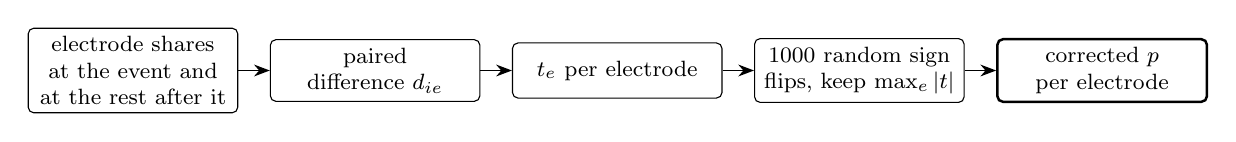
\begin{tikzpicture}[node distance=4mm and 4mm, font=\footnotesize, box/.append style={text width=2.45cm}]
\node[box] (a) {electrode shares at the event and at the rest after it};
\node[box, right=of a] (b) {paired difference $d_{ie}$};
\node[box, right=of b] (c) {$t_e$ per electrode};
\node[box, right=of c] (d) {1000 random sign flips, keep $\max_e |t|$};
\node[result, right=of d] (e) {corrected $p$ per electrode};
\draw[arr] (a)--(b); \draw[arr] (b)--(c); \draw[arr] (c)--(d); \draw[arr] (d)--(e);
\end{tikzpicture}
\end{latin}

\caption{مقایسه‌ی رخداد با استراحت.}
\end{figure}

\subsection{سنجش خودِ روش‌ها}

هر روش تفسیری یک نقشه می‌دهد، ولی این به معنای درست بودن نقشه نیست. دو آزمون می‌سنجند که نقشه‌ها واقعاً چیزی درباره‌ی مدل آموزش‌دیده می‌گویند.

\textbf{\lr{deletion check}} \cite{samek2017}. اگر یک روش درست بگوید کدام ورودی‌ها مهم‌اند، حذف همان ورودی‌ها باید خروجی را بیشتر از حذف ورودی‌های تصادفی تغییر دهد. «حذف» یعنی صفر کردن، که چون داده‌ها استانداردند برابر میانگین آموزش است. برای \lr{EEG} هر خانه یک الکترود در یک \lr{token} است (هر چهار باند با هم)، و برای سینماتیک همه‌ی ویژگی‌های یک \lr{token}. ۵، ۱۰، ۲۰ و ۴۰ درصد از مهم‌ترین خانه‌ها حذف و با حذف همان تعداد خانه‌ی تصادفی (میانگین ۱۰ بار) مقایسه می‌شوند:
\begin{equation}
\Delta_{top}(q)=\big|\,y(x)-y(x_{\setminus \mathrm{top}(q)})\,\big|,\qquad \Delta_{rand}(q)=\operatorname{mean}_{10}\big|\,y(x)-y(x_{\setminus \mathrm{rand}(q)})\,\big|.
\end{equation}
$x_{\setminus \mathrm{top}(q)}$ ورودی بدون $q$ درصد خانه‌های برتر است و $x_{\setminus \mathrm{rand}(q)}$ ورودی بدون همان تعداد خانه‌ی تصادفی. هر چه $\Delta_{top}$ یک روش بزرگ‌تر باشد، آن روش ورودی‌های واقعاً اثرگذار را بهتر پیدا کرده است.

\textbf{\lr{weight-shuffle check}} \cite{adebayo2018}. یک نسخه از مدل ساخته می‌شود که درایه‌های هر ماتریس وزن آن به‌هم ریخته شده است؛ یعنی مدلی با همان معماری که هیچ چیز یاد نگرفته. نقشه‌ها برای این مدل هم ساخته و با نقشه‌های مدل واقعی مقایسه می‌شوند (\lr{Spearman correlation}). اگر نقشه‌ی مدل به‌هم‌ریخته هم همان شکل را داشته باشد، آن شکل از معماری آمده و نه از آنچه مدل یاد گرفته؛ پس درباره‌ی داده چیزی نمی‌گوید. همبستگی خوب نزدیک صفر است.

\begin{figure}[htbp]
\centering
% Deletion check (top) and weight-shuffle check (bottom).
\begin{latin}
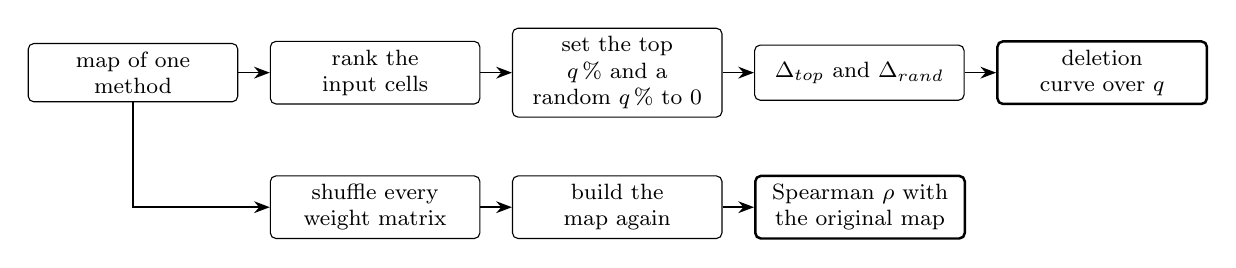
\begin{tikzpicture}[node distance=4mm and 4mm, font=\footnotesize, box/.append style={text width=2.45cm}]
\node[box] (a) {map of one method};
\node[box, right=of a] (b) {rank the input cells};
\node[box, right=of b] (c) {set the top $q$\,\% and a random $q$\,\% to 0};
\node[box, right=of c] (d) {$\Delta_{top}$ and $\Delta_{rand}$};
\node[result, right=of d] (e) {deletion curve over $q$};
\draw[arr] (a)--(b); \draw[arr] (b)--(c); \draw[arr] (c)--(d); \draw[arr] (d)--(e);
\node[box, below=9mm of b] (f) {shuffle every weight matrix};
\node[box, right=of f] (g) {build the map again};
\node[result, right=of g] (h) {Spearman $\rho$ with the original map};
\draw[arr] (a.south)|-(f.west); \draw[arr] (f)--(g); \draw[arr] (g)--(h);
\end{tikzpicture}
\end{latin}

\caption{\lr{deletion check} (بالا) و \lr{weight-shuffle check} (پایین).}
\end{figure}

\subsection{نتایج برای همه‌ی شرکت‌کننده‌ها}

\paragraph{کدام روش ورودی‌های مهم را بهتر پیدا می‌کند؟} جدول~\ref{tab:interp-del} پاسخ \lr{deletion check} است. برای \lr{E}، \lr{gradient-weighted rollout} با فاصله‌ی زیاد بهترین روش است: حذف خانه‌های برتر آن خروجی را \lr{۰٫۲۰۵} تغییر می‌دهد، در حالی که این عدد برای روش‌های دیگر حدود \lr{۰٫۰۹} و برای حذف تصادفی \lr{۰٫۰۲۱} است. این روش در هر ۱۲ شرکت‌کننده اول است (جدول~\ref{tab:interp-parts}). برای \lr{K}، سه روش \lr{rollout}، \lr{gradient-weighted rollout} و \lr{gradient × input} تقریباً برابرند و \lr{attention flow} ضعیف‌تر است. همه‌ی روش‌ها از حذف تصادفی بهترند.

\begin{table}[htbp]
\centering
\small
\caption{\lr{deletion check}، میانگین روی ۱۲ شرکت‌کننده، پنج عضله و چهار کسر حذف (۵، ۱۰، ۲۰ و ۴۰ درصد): تغییر خروجی (واحد مدل) وقتی ورودی‌هایی که هر روش مهم‌تر می‌داند حذف می‌شوند. بزرگ‌تر بهتر است.}
\label{tab:interp-del}
\begin{tabular}{cccccc}
\toprule
خروجی & حذف تصادفی & \lr{rollout} & \lr{attention flow} & \lr{gradient-weighted rollout} & \lr{gradient × input} \\
\midrule
\lr{E} & \lr{۰٫۰۲۱} & \lr{۰٫۰۹۸} & \lr{۰٫۰۹۳} & \lr{۰٫۲۰۵} & \lr{۰٫۰۹۲} \\
\lr{K} & \lr{۰٫۰۳۷} & \lr{۰٫۲۱۲} & \lr{۰٫۱۱۸} & \lr{۰٫۲۱۳} & \lr{۰٫۲۱۱} \\
\bottomrule
\end{tabular}
\end{table}


\paragraph{کدام نقشه‌ها واقعاً از یادگیری می‌آیند؟} جدول~\ref{tab:interp-sanity} یک هشدار دارد. \lr{plain rollout} \lr{K} برای مدل به‌هم‌ریخته هم شکل مشابهی دارد (همبستگی اسپیرمن \lr{۰٫۴۷}). دلیلش ساختار مدل است: \lr{residual connection} و ردپای \lr{stem} همیشه بیشترین سهم را به \lr{token} خودِ رخداد و همسایه‌هایش می‌دهند، چه مدل آموزش دیده باشد چه نه. برای \lr{E}، \lr{gradient × input} کمترین وابستگی به یادگیری را دارد (\lr{۰٫۲۷}). \lr{gradient-weighted rollout} در هر دو خروجی نزدیک صفر است.

نتیجه‌ی این دو آزمون با هم: \lr{gradient-weighted rollout} هم ورودی‌های مهم را بهتر پیدا می‌کند و هم کمتر از ساختار مدل اثر می‌گیرد. برای همین روش اصلی ادعاهای این گزارش است.

\begin{table}[htbp]
\centering
\small
\caption{\lr{weight-shuffle check}: \lr{Spearman correlation} بین نقشه‌ی مدل آموزش‌دیده و نقشه‌ی مدلی با ماتریس‌های وزنِ به‌هم‌ریخته (میانگین روی ۱۲ شرکت‌کننده). نزدیک صفر بهتر است: یعنی نقشه به آموخته‌های مدل وابسته است.}
\label{tab:interp-sanity}
\begin{tabular}{ccccc}
\toprule
خروجی & \lr{rollout} & \lr{attention flow} & \lr{gradient-weighted rollout} & \lr{gradient × input} \\
\midrule
\lr{E} & \lr{۰٫۰۳۶} & \lr{۰٫۰۷۵} & \lr{۰٫۰۱۲} & \lr{۰٫۲۷۱} \\
\lr{K} & \lr{۰٫۴۷۳} & \lr{−۰٫۰۰۸} & \lr{۰٫۰۷۰} & \lr{۰٫۰۷۶} \\
\bottomrule
\end{tabular}
\end{table}

\begin{table}[htbp]
\centering
\small
\caption{اجزای دقیق خروجی در پنجره‌های رخداد و بهترین روش تفسیر برای \lr{E} در هر شرکت‌کننده.}
\label{tab:interp-parts}
\begin{tabular}{ccccc}
\toprule
شرکت‌کننده & بازه‌ی \lr{history gain} & $|F_{eeg}|/K$ (\%) & بیشینه‌ی $|g|$ & بهترین روش در \lr{deletion check} (\lr{E}) \\
\midrule
\lr{P1} & \lr{۱٫۰۹}--\lr{۱٫۲۰} & \lr{۰٫۶۹} & \lr{۰٫۰۱۵} & \lr{gradient-weighted rollout} \\
\lr{P2} & \lr{۱٫۰۶}--\lr{۱٫۱۳} & \lr{۰٫۱۵} & \lr{۰٫۰۱۴} & \lr{gradient-weighted rollout} \\
\lr{P3} & \lr{۱٫۱۰}--\lr{۱٫۱۸} & \lr{۱٫۰۱} & \lr{۰٫۰۱۷} & \lr{gradient-weighted rollout} \\
\lr{P4} & \lr{۱٫۱۰}--\lr{۱٫۱۹} & \lr{۰٫۶۰} & \lr{۰٫۰۲۶} & \lr{gradient-weighted rollout} \\
\lr{P5} & \lr{۱٫۰۴}--\lr{۱٫۱۱} & \lr{۰٫۵۷} & \lr{۰٫۰۲۶} & \lr{gradient-weighted rollout} \\
\lr{P6} & \lr{۱٫۰۸}--\lr{۱٫۱۵} & \lr{۱٫۱۴} & \lr{۰٫۰۲۴} & \lr{gradient-weighted rollout} \\
\lr{P7} & \lr{۱٫۱۱}--\lr{۱٫۱۸} & \lr{۰٫۹۱} & \lr{۰٫۰۱۸} & \lr{gradient-weighted rollout} \\
\lr{P8} & \lr{۱٫۰۸}--\lr{۱٫۱۸} & \lr{۲٫۲۲} & \lr{۰٫۰۴۲} & \lr{gradient-weighted rollout} \\
\lr{P9} & \lr{۱٫۰۸}--\lr{۱٫۱۸} & \lr{۰٫۶۵} & \lr{۰٫۰۱۲} & \lr{gradient-weighted rollout} \\
\lr{P10} & \lr{۱٫۰۹}--\lr{۱٫۲۶} & \lr{۰٫۸۳} & \lr{۰٫۰۱۰} & \lr{gradient-weighted rollout} \\
\lr{P11} & \lr{۱٫۰۸}--\lr{۱٫۱۴} & \lr{۱٫۰۹} & \lr{۰٫۰۱۵} & \lr{gradient-weighted rollout} \\
\lr{P12} & \lr{۱٫۰۹}--\lr{۱٫۱۷} & \lr{۱٫۰۶} & \lr{۰٫۰۲۱} & \lr{gradient-weighted rollout} \\
\bottomrule
\end{tabular}
\end{table}


\subsection{نتایج \lr{P1} و \lr{P2}: هر شکل چه می‌گوید}
\label{sec:interp-figs}

همه‌ی شکل‌های این بخش برای رخداد «جدا شدن» (\lr{lift\_off}) و میانگین روی همه‌ی بلندکردن‌های سری‌های آزمون هستند. شکل‌ها بر اساس نوعشان دسته‌بندی شده‌اند و از هر نوع، شکل \lr{P1} و \lr{P2} کنار هم آمده تا بتوان دو نفر را مقایسه کرد. برای هر نوع شکل سه چیز توضیح داده می‌شود: چه چیزی رسم شده، چطور خوانده می‌شود و چه نتیجه‌ای از آن می‌گیریم.

\subsubsection*{۱. شکل زمانی \lr{K}: مدل سینماتیک به کدام لحظه‌ها نگاه می‌کند؟}

\textbf{چه رسم شده.} پنج پنل بالا یکی برای هر عضله است. محور افقی زمان نسبت به لحظه‌ی جدا شدن است، از ۴ ثانیه قبل تا ۴ ثانیه بعد (کل پنجره‌ی ۸ ثانیه‌ای مدل). محور عمودی سهم هر \lr{token} ورودی در پیش‌بینی \lr{K} در لحظه‌ی صفر است. آبی \lr{rollout} و سبز \lr{gradient-weighted rollout} است و نوار کم‌رنگ دور هر منحنی \lr{SEM} روی بلندکردن‌هاست. سهم خودِ \lr{token} رخداد و همسایه‌هایش بالای هر پنل به‌صورت عدد نوشته شده (\mbox{«\lr{own token: 14\%}»}) و منحنی سهم بقیه‌ی \lr{tokens} است. پنل پایین \lr{attention flow} منهای جریان توجه یکنواخت است؛ صفر یعنی «مثل مدلی که به همه‌جا یکسان نگاه می‌کند» و منفی یعنی مدل راه آن لحظه را تنگ کرده است.

\textbf{چطور بخوانیم.} جایی که منحنی بالاتر است، مدل برای پیش‌بینی فعالیت عضله در لحظه‌ی جدا شدن بیشتر از اطلاعات آن لحظه استفاده کرده است. اگر منحنی صاف بود، یعنی همه‌ی لحظه‌ها به یک اندازه مهم بودند و مدل جای خاصی را ترجیح نمی‌داد.

\textbf{چه می‌فهمیم.} در هر دو نفر الگو یکی است و سه بخش دارد:
\begin{itemize}
\item \textbf{پیش از رخداد (۴ ثانیه تا صفر):} سهم بالاست. در \lr{P2} از حدود ۲ ثانیه پیش از جدا شدن بالا می‌رود و درست پیش از صفر به اوج می‌رسد. این همان بازه‌ای است که دست به جسم می‌رسد، آن را می‌گیرد و نیروی بار را بالا می‌برد. پس \lr{K} برای پیش‌بینی فعالیت عضله در لحظه‌ی جدا شدن، به حرکت و نیروی پیش از آن نگاه می‌کند.
\item \textbf{۰ تا حدود \lr{۲٫۵} ثانیه بعد:} سهم کمترین است و جریان هم بیشترین افت را دارد (در \lr{P2} تا \lr{−۰٫۴۵}). این بازه آغاز نگه‌داشتن است، اما آن لحظه‌ها هنوز بعد از رخدادند و برای توضیح فعالیت در لحظه‌ی جدا شدن اطلاعات تازه‌ای ندارند.
\item \textbf{حدود ۳ تا ۴ ثانیه بعد:} سهم دوباره بالا می‌رود. بخشی از این افزایش اثر لبه‌ی پنجره است که در همه‌ی افراد دیده می‌شود (بخش~\ref{sec:consistency}) و نباید آن را به رویداد حرکتی نسبت داد.
\end{itemize}
منحنی آبی در پنج پنل تقریباً یکی است، چون \lr{rollout} زمانی به عضله بستگی ندارد. منحنی سبز برای هر عضله قله‌های خودش را دارد؛ مثلاً در \lr{P1} \lr{ED} قله‌ی بلندی حدود \lr{۰٫۸} ثانیه پیش از رخداد دارد. یعنی گرادیان نشان می‌دهد هر عضله به لحظه‌ی کمی متفاوتی از حرکت حساس است.

\fig{P1_time_K_lift_off.png}{1.0}{\lr{P1}، خروجی \lr{K}: سهم هر \lr{token} زمانی در اطراف جدا شدن جسم (بالا) و \lr{attention flow} منهای \lr{uniform-attention flow} (پایین).}
\fig{P2_time_K_lift_off.png}{1.0}{\lr{P2}، خروجی \lr{K}: سهم زمانی و \lr{attention flow} منهای خط پایه. همان الگوی \lr{P1}: سهم بالا پیش از رخداد، کمترین سهم در ۰ تا \lr{۲٫۵} ثانیه بعد.}

\subsubsection*{۲. شکل زمانی \lr{E}: مدل \lr{EEG} به کدام لحظه‌ها نگاه می‌کند؟}

\textbf{چه رسم شده.} مثل شکل قبل، اما برای خروجی \lr{E} که فقط \lr{EEG} می‌بیند.

\textbf{چه می‌فهمیم.} سه تفاوت با \lr{K} دارد:
\begin{itemize}
\item \textbf{سهم خودِ لحظه بیشتر است:} در \lr{P1} حدود ۲۶ درصد در برابر ۱۴ درصد برای \lr{K}. یعنی \lr{E} بیشتر به توان باندهای \lr{EEG} در همان لحظه تکیه می‌کند و کمتر به گذشته.
\item \textbf{منحنی صاف‌تر است:} سهم لحظه‌های دیگر تقریباً یکسان است و ساختار زمانی روشنی مثل \lr{K} ندارد. در \lr{P1} سبز کمی پیش از صفر بالا می‌رود که با زمان‌بندی \lr{ERD} پیش از حرکت سازگار است. در \lr{P2} حتی این هم دیده نمی‌شود.
\item \textbf{جهش‌های تیز در اواخر پنجره:} در \lr{P1} یک قله‌ی تیز حدود \lr{۳٫۲} ثانیه بعد از رخداد هست و در \lr{P2} جهش در لبه‌ی پنجره. چون این قله‌ها در همه‌ی افراد در یک زمان نیستند (بخش~\ref{sec:consistency})، نمی‌توان آن‌ها را به یک رویداد حرکتی مشخص نسبت داد.
\end{itemize}
پنل جریان برای \lr{E} تقریباً صاف و همه‌جا حدود \lr{−۰٫۲} است. یعنی جریان در مسیر \lr{EEG} درباره‌ی زمان تقریباً چیزی نمی‌گوید.

\fig{P1_time_E_lift_off.png}{1.0}{\lr{P1}، خروجی \lr{E}: سهم زمانی و \lr{attention flow} منهای خط پایه. سهم خودِ لحظه ۲۶ درصد است، بیشتر از \lr{K}.}
\fig{P2_time_E_lift_off.png}{1.0}{\lr{P2}، خروجی \lr{E}: سهم زمانی و \lr{attention flow} منهای خط پایه. منحنی تقریباً صاف است و فقط در لبه‌ی پنجره جهش دارد.}

\subsubsection*{۳. نقشه‌ی سر: \lr{E} از کدام الکترودها اطلاعات می‌گیرد؟}

\textbf{چه رسم شده.} هر دایره سر از بالاست (بینی بالا، گوش‌ها در دو طرف) و نقطه‌ها جای ۳۲ الکترود. رنگ سهم هر الکترود است: هر چه تیره‌تر، سهم بیشتر. سهم یکنواخت برای هر الکترود $1/32\approx0.031$ است؛ پس رنگ‌های تیره‌تر از وسط نوار رنگ یعنی سهمی بیشتر از حالت یکنواخت. اولین دایره \lr{rollout} است (برای همه‌ی عضله‌ها یکی) و پنج دایره‌ی بعد \lr{gradient-weighted rollout} برای هر عضله. بین الکترودها درون‌یابی شده تا نقشه پیوسته دیده شود.

\textbf{چطور بخوانیم.} کانون‌های تیره جاهایی‌اند که \lr{E} بیشترین اطلاعات را از آن‌ها گرفته است. ناحیه‌ی مرکزی چپ (\lr{C3}، \lr{FC5}، \lr{CP5}) بالای قشر حرکتی دست راست است و انتظار داریم آنجا مهم باشد. پیشانی (\lr{Fp1}، \lr{Fp2}، \lr{F7}، \lr{F8}) به حرکت چشم حساس است، و پس‌سری و گیجگاهی (\lr{O1}، \lr{O2}، \lr{PO9}، \lr{PO10}، \lr{TP9}، \lr{TP10}) به پردازش بینایی و فعالیت عضلات گردن.

\textbf{چه می‌فهمیم.}
\begin{itemize}
\item در \lr{P1} قوی‌ترین کانون روی مرکزی چپ است؛ یعنی همان جایی که از نظر فیزیولوژی انتظار داریم. کانون کوچک‌تری روی مرکزی راست (\lr{C4}) و کانون قوی دیگری روی پس‌سری هم هست.
\item در \lr{P2} کانون مرکزی چپ ضعیف‌تر است و بیشترین سهم روی لبه‌های سر، به‌خصوص پیشانی راست و پس‌سری، است. این نشانه‌ی احتمال \lr{artifact} است.
\item پنج نقشه‌ی عضله‌ها در هر نفر تقریباً یکسان‌اند. پس \lr{E} برای همه‌ی عضله‌ها از یک جای سر می‌خواند و نقشه‌ی خاص هر عضله نمی‌سازد؛ این با خواندن «مرحله‌ی کلی حرکت» سازگار است، نه فرمان جداگانه برای هر عضله.
\item در \lr{P1} نقشه‌ی \lr{attention flow} رسم نشده، چون سهم همه‌ی الکترودها بین \lr{۳٫۰۹} و \lr{۳٫۱۵} درصد است و نقشه چیزی جز رنگ یکسان نشان نمی‌داد. در \lr{P2} رسم شده، اما نوار رنگش فقط از \lr{۰٫۰۲۹} تا \lr{۰٫۰۳۲} است؛ تفاوت‌ها بسیار کوچک‌اند.
\end{itemize}

\fig{P1_scalp_E_lift_off.png}{1.0}{\lr{P1}، خروجی \lr{E}: سهم هر الکترود در \lr{rollout} و در \lr{gradient-weighted rollout} برای هر عضله. کانون اصلی روی مرکزی چپ (\lr{C3}). نقشه‌ی \lr{attention flow} رسم نشده، چون برای همه‌ی الکترودها تقریباً برابر است.}
\fig{P2_scalp_E_lift_off.png}{1.0}{\lr{P2}، خروجی \lr{E}: سهم هر الکترود. کانون مرکزی چپ ضعیف‌تر و سهم لبه‌های سر بیشتر است. جریان الکترودها کمی پراکندگی دارد (\lr{۱۱٫۵} درصد)، پس نقشه‌اش با رنگ از کمینه تا بیشینه رسم شده است.}

\subsubsection*{۴. توجه هر لایه‌ی \lr{electrode graph}: الکترودها از هم چه می‌خوانند؟}

\textbf{چه رسم شده.} دو ماتریس $32\times32$، یکی برای هر لایه‌ی \lr{electrode graph}، در لحظه‌ی جدا شدن و میانگین روی سرها. هر سطر الکترودی است که اطلاعات می‌گیرد و هر ستون الکترودی که اطلاعات می‌دهد. جمع هر سطر ۱ است.

\textbf{چطور بخوانیم.} یک ستون تیره که از بالا تا پایین ادامه دارد یعنی همه‌ی الکترودها از همان یک الکترود می‌خوانند؛ آن الکترود یک «مرکز پخش» است. قطر تیره یعنی هر الکترود بیشتر اطلاعات خودش را نگه می‌دارد.

\textbf{چه می‌فهمیم.} لایه‌ی اول در هر دو نفر چند مرکز پخش دارد و لایه‌ی دوم بیشتر قطری است. یعنی لایه‌ی اول اطلاعات چند الکترود خاص را به همه می‌رساند و لایه‌ی دوم آن را با اطلاعات خود هر الکترود ترکیب می‌کند. نکته‌ی مهم این است که مرکزها کدام‌اند:
\begin{itemize}
\item در \lr{P1}: \lr{C3} (قشر حرکتی چپ) و \lr{O1}/\lr{PO9} (پس‌سری). \lr{C3} در لایه‌ی دوم هم یک ستون تیره دارد.
\item در \lr{P2}: \lr{F8} و \lr{F7} (پیشانی، نزدیک چشم‌ها) و \lr{PO10}/\lr{TP10} (پشت گوش و گردن).
\end{itemize}
این شکل توضیح می‌دهد نقشه‌ی سر از کجا آمده است: نقشه‌ی \lr{P1} بیشتر از قشر حرکتی می‌آید و نقشه‌ی \lr{P2} بیشتر از الکترودهایی که به حرکت چشم و عضلات گردن حساس‌اند. پس اطلاعات \lr{E} در \lr{P2} احتمالاً بیشتر از \lr{artifact} است تا از قشر حرکتی.

\fig{P1_electrode_layers_lift_off.png}{0.8}{\lr{P1}: توجه دو لایه‌ی \lr{electrode graph} در لحظه‌ی جدا شدن (سطر = الکترود گیرنده). مرکزهای پخش در لایه‌ی اول: \lr{C3} و \lr{O1}.}
\fig{P2_electrode_layers_lift_off.png}{0.8}{\lr{P2}: توجه دو لایه‌ی \lr{electrode graph} در لحظه‌ی جدا شدن. مرکزهای پخش در لایه‌ی اول: \lr{F8}، \lr{F7} و \lr{PO10}.}

\subsubsection*{۵. \lr{muscle graph}: عضله‌ها از هم اطلاعات می‌گیرند؟}

\textbf{چه رسم شده.} چهار ماتریس $5\times5$: \lr{rollout} و \lr{gradient-weighted rollout} (\lr{relevance}) برای \lr{K} و \lr{E}. سطر عضله‌ی گیرنده و ستون عضله‌ی فرستنده است.

\textbf{چطور بخوانیم.} قطر تیره یعنی هر عضله پیش‌بینی‌اش را بیشتر از گره خودش می‌سازد. خانه‌ی تیره بیرون قطر، مثلاً سطر \lr{AD} و ستون \lr{ED}، یعنی پیش‌بینی \lr{AD} از اطلاعات گره \lr{ED} هم استفاده کرده است.

\textbf{چه می‌فهمیم.} در هر دو نفر و هر دو خروجی قطر غالب است؛ عضله‌ها بیشتر مستقل پیش‌بینی می‌شوند. در \lr{rollout} خانه‌های بیرون قطر تقریباً یکسان‌اند و الگوی خاصی ندارند. در \lr{relevance} چند خانه‌ی بیرون قطر برجسته می‌شوند؛ مثلاً در \lr{P1} \lr{AD} از \lr{ED} برای \lr{K}، و \lr{BR} از \lr{FD} برای \lr{E}. اما این رابطه‌ها از یک نفر به نفر دیگر عوض می‌شوند و بخش~\ref{sec:consistency} نشان می‌دهد در \lr{E} یکسانی‌شان بین افراد کم است. پس نباید آن‌ها را هم‌کاری ثابت عضله‌ها تعبیر کرد.

\fig{P1_muscle_graph_lift_off.png}{0.95}{\lr{P1}: \lr{muscle graph} در لحظه‌ی جدا شدن برای \lr{K} و \lr{E}، با \lr{rollout} و \lr{gradient-weighted rollout}.}
\fig{P2_muscle_graph_lift_off.png}{0.95}{\lr{P2}: \lr{muscle graph} در لحظه‌ی جدا شدن.}

\subsubsection*{۶. مقایسه با استراحت: کدام الکترود فقط هنگام حرکت مهم می‌شود؟}

\textbf{چه رسم شده.} برای هر عضله یک نقشه‌ی سر. رنگ آماره‌ی $t$ جفت‌شده است: سهم الکترود در لحظه‌ی جدا شدن منهای سهمش در استراحت بعد از همان بلندکردن. قرمز یعنی در رخداد سهم بیشتری دارد، آبی یعنی در استراحت. دایره‌های توخالی الکترودهایی‌اند که اختلافشان پس از تصحیح برای ۳۲ الکترود معنادار است.

\textbf{چطور بخوانیم.} نقشه‌ی سر (شکل نوع ۳) فقط می‌گوید \lr{E} از کجا می‌خواند؛ ممکن است همان الکترود در استراحت هم همان‌قدر مهم باشد. این شکل جواب می‌دهد کدام الکترودها \emph{مخصوص لحظه‌ی حرکت} مهم می‌شوند.

\textbf{چه می‌فهمیم.} نتیجه بین دو نفر و حتی بین عضله‌های یک نفر بسیار متفاوت است. در \lr{P1} بیشترین الکترودهای معنادار برای \lr{FD} است (پیشانی قرمز، پس‌سری آبی) و برای بقیه‌ی عضله‌ها چند الکترود پراکنده. در \lr{P2} برای همه‌ی عضله‌ها پس‌سری (\lr{O1}، \lr{O2}، \lr{P7}، \lr{P8}) قرمز و معنادار است و پیشانی راست آبی. افزایش سهم پس‌سری درست هنگام جدا شدن جسم با نگاه کردن به جسم و پردازش بینایی سازگار است، نه با فرمان حرکتی. بخش~\ref{sec:consistency} این را تأیید می‌کند: این نقشه‌ها بین افراد تقریباً شبیه نیستند (\lr{pairwise $\rho$} حدود \lr{۰٫۰۶})، پس برای نتیجه‌گیری گروهی مناسب نیستند.

\fig{P1_rest_contrast_lift_off.png}{0.95}{\lr{P1}: سهم الکترودها در \lr{E} هنگام جدا شدن منهای استراحت بعد از آن؛ آماره‌ی $t$ جفت‌شده. دایره‌ها الکترودهایی‌اند که $p$ تصحیح‌شده‌شان کمتر از \lr{۰٫۰۵} است.}
\fig{P2_rest_contrast_lift_off.png}{0.95}{\lr{P2}: مقایسه‌ی رخداد با استراحت برای \lr{E}. پس‌سری در همه‌ی عضله‌ها هنگام جدا شدن سهم بیشتری دارد.}

\subsubsection*{۷. سهم ورودی‌ها: کدام ویژگی‌ها و کدام باندها؟}

\textbf{چه رسم شده.} سه نمودار میله‌ای از \lr{gradient × input}، میانگین روی پنج عضله. چپ: سهم هر یک از ۳۲ ویژگی \lr{K} (۲۴ ویژگی سینماتیک و ۸ ویژگی تاریخچه، با نام‌های کد؛ پیشوند \lr{v\_} یعنی سرعت). وسط: سهم چهار باند \lr{EEG} در \lr{E}. راست: سهم همان چهار باند در اصلاح \lr{EEG} درون \lr{F}. سهم‌های هر نمودار جمع ۱ دارند.

\textbf{چطور بخوانیم.} این تنها شکلی است که درباره‌ی \emph{نوع} ورودی می‌گوید، نه جای آن در زمان یا روی سر. میله‌ی بلندتر یعنی تغییر کوچک آن ویژگی خروجی را بیشتر تغییر می‌دهد.

\textbf{چه می‌فهمیم.}
\begin{itemize}
\item \textbf{\lr{K} از فیزیک بلند کردن استفاده می‌کند.} در \lr{P1} بیشترین سهم با ارتفاع شست و انگشت اشاره (\lr{p\_thumb\_z}، \lr{p\_index\_z}) و سرعت نیروی بار و گرفتن (\lr{v\_F\_L\_gated}، \lr{v\_F\_G\_gated}) است. در \lr{P2} خود دو نیرو (\lr{F\_G\_gated}، \lr{F\_L\_gated}) و سرعت باز و بسته شدن دست (\lr{v\_d\_grip}) جلوترند. لحظه‌ی جدا شدن دقیقاً جایی است که نیروی بار به وزن جسم می‌رسد و دست بالا می‌رود، پس این ویژگی‌ها همان چیزی‌اند که از فیزیک انتظار داریم.
\item \textbf{تاریخچه کمک می‌کند ولی نقش اصلی ندارد.} هشت ویژگی تاریخچه (از \lr{has history} تا \lr{mean grip}) هر کدام ۱ تا ۵ درصد سهم دارند. \lr{has history} از همه بیشتر است؛ یعنی مدل بلندکردن اول سری را از بقیه جدا می‌کند.
\item \textbf{\lr{E} باند بتا را ترجیح می‌دهد.} در هر دو نفر بتا (۱۳ تا ۳۰ هرتز) اول است و گامای پایین (۳۰ تا ۴۰ هرتز) دوم. بتا با پژوهش‌های قشر حرکتی می‌خواند. سهم بالای گامای پایین به \lr{artifact} عضلات سر حساس است.
\item \textbf{اصلاح \lr{EEG} در \lr{F} همان باندهای \lr{E} را می‌خواند.} نمودار راست تقریباً تکرار نمودار وسط است. پس \lr{fusion} اطلاعات دیگری از \lr{EEG} نمی‌گیرد، فقط همان را با \lr{gate} نزدیک صفر اضافه می‌کند.
\end{itemize}

\fig{P1_inputs_lift_off.png}{0.85}{\lr{P1}: سهم ویژگی‌های سینماتیک و تاریخچه در \lr{K} و سهم باندهای \lr{EEG} در \lr{E} و در اصلاح \lr{EEG} درون \lr{F} (\lr{gradient × input}).}
\fig{P2_inputs_lift_off.png}{0.85}{\lr{P2}: سهم ورودی‌ها (\lr{gradient × input}).}

\subsubsection*{۸. \lr{deletion check}: کدام روش تفسیر را باور کنیم؟}

\textbf{چه رسم شده.} محور افقی درصد ورودی‌هایی است که حذف شده‌اند (۵، ۱۰، ۲۰ و ۴۰ درصد)، به ترتیبی که هر روش مهم‌تر می‌داند. محور عمودی تغییر خروجی مدل در اثر این حذف است. هر رنگ یک روش است و خاکستری حذف تصادفی. چپ \lr{E} و راست \lr{K}.

\textbf{چطور بخوانیم.} این شکل خود روش‌ها را می‌سنجد، نه مدل را. روشی که واقعاً ورودی‌های مهم را پیدا کرده باشد، با حذف همان ۵ درصد اول باید خروجی را بسیار تغییر دهد؛ یعنی منحنی‌اش از همان ابتدا بالا باشد. منحنی نزدیک خاکستری یعنی آن روش بهتر از انتخاب تصادفی نیست.

\textbf{چه می‌فهمیم.}
\begin{itemize}
\item \textbf{برای \lr{E}:} سبز (\lr{gradient-weighted rollout}) در هر دو نفر از همان ۵ درصد اول بسیار بالاتر از بقیه است (در \lr{P1} حدود \lr{۰٫۲۸} در برابر حدود \lr{۰٫۰۸}). پس برای \lr{EEG} فقط این روش ورودی‌های مهم را دقیق رتبه‌بندی می‌کند. در \lr{P2} سبز بعد از ۲۰ درصد کمی پایین می‌آید؛ احتمالاً با حذف ورودی‌های بیشتر، اثرهای مخالف هم حذف می‌شوند و یکدیگر را خنثی می‌کنند.
\item \textbf{برای \lr{K}:} سه روش \lr{rollout}، \lr{gradient-weighted rollout} و \lr{gradient × input} تقریباً روی هم‌اند. در \lr{P1} منحنی آن‌ها از ۵ درصد صاف است؛ یعنی تقریباً همه‌ی اثر در همان ۵ درصد اول است (خودِ لحظه‌ی رخداد و همسایه‌هایش) و حذف بیشتر چیزی اضافه نمی‌کند. \lr{attention flow} در \lr{P1} از ۵ درصد بسیار پایین شروع می‌شود، چون تقریباً به همه‌ی ورودی‌ها سهم برابر می‌دهد و نمی‌داند کدام را اول حذف کند.
\item همه‌ی روش‌ها در هر دو نفر بالاتر از حذف تصادفی‌اند؛ پس هیچ‌کدام بی‌معنا نیستند، فقط دقتشان فرق دارد.
\end{itemize}

\fig{P1_deletion.png}{0.75}{\lr{P1}: منحنی‌های \lr{deletion check}. منحنی بالاتر در درصدهای کم یعنی روش دقیق‌تر.}
\fig{P2_deletion.png}{0.75}{\lr{P2}: منحنی‌های \lr{deletion check}.}
\clearpage

\section{\lr{attention rollout} و \lr{attention flow}}
\label{sec:rollout-flow}

\lr{attention rollout} و \lr{attention flow} \cite{abnar2020} هر دو یک پرسش را پاسخ می‌دهند: یک عدد خروجی از کدام ورودی‌ها آمده است، وقتی اطلاعات در هر لایه فقط از راه توجه و \lr{residual connection} بین موقعیت‌ها جابه‌جا می‌شود. هر دو روی همان ماتریس‌های ثبت‌شده کار می‌کنند و فقط در قاعده‌ی ترکیب لایه‌ها فرق دارند: \lr{rollout} در طول هر مسیر وزن‌ها را ضرب و مسیرها را جمع می‌کند، و \lr{attention flow} وزن‌ها را ظرفیت لوله می‌گیرد و بیشینه‌ی جریانی را که از یک ورودی به خروجی می‌رسد حساب می‌کند. قاعده‌ی «یک مخلوط‌کننده» در \lr{v2} (بخش~\ref{sec:v2}) شرط لازم هر دو است: چون اطلاعات جز از راه توجه (و \lr{stem} معلوم \lr{K}) بین موقعیت‌ها جابه‌جا نمی‌شود، این گراف کل مسیر اطلاعات را می‌پوشاند.

\subsection{نمادگذاری و \lr{layered graph}}

برای لایه‌ی $l$ از $L$ لایه‌ی توجه، \lr{recorder} ماتریس $A^{h}_l\in\mathbb{R}^{n\times n}$ را برای هر سر $h=1,\dots,H$ پس از \lr{softmax} برمی‌دارد؛ سطر $i$ گیرنده (پرسش) و ستون $j$ فرستنده است و هر سطر جمع ۱ دارد. میانگین سرها و \lr{residual connection}:
\begin{equation}
\overline{A}_l=\frac1H\sum_{h=1}^{H}A^{h}_l,\qquad \hat A_l=\tfrac12\,\overline{A}_l+\tfrac12 I .
\label{eq:ahat}
\end{equation}
وزن $\tfrac12$ برای \lr{residual connection} یک قرارداد است: بلوک $x+\mathrm{Attn}(\mathrm{LN}(x))$ نیمی از اطلاعات را از مسیر توجه و نیمی را از مسیر مستقیم فرض می‌کند. \lr{layered graph} $L+1$ ردیف گره دارد (ردیف ۰ ورودی‌ها، ردیف $L$ خروجی‌ها) و از گره $j$ در ردیف $l-1$ به گره $i$ در ردیف $l$ یک یال با وزن $\hat A_l[i,j]$ می‌رود. یال‌های $j\to j$ مسیر اتصال باقی‌مانده‌اند و بقیه مسیر توجه (شکل~\ref{fig:layered}).

\begin{figure}[htbp]
\centering
% Layered graph of rollout and attention flow.
\begin{latin}
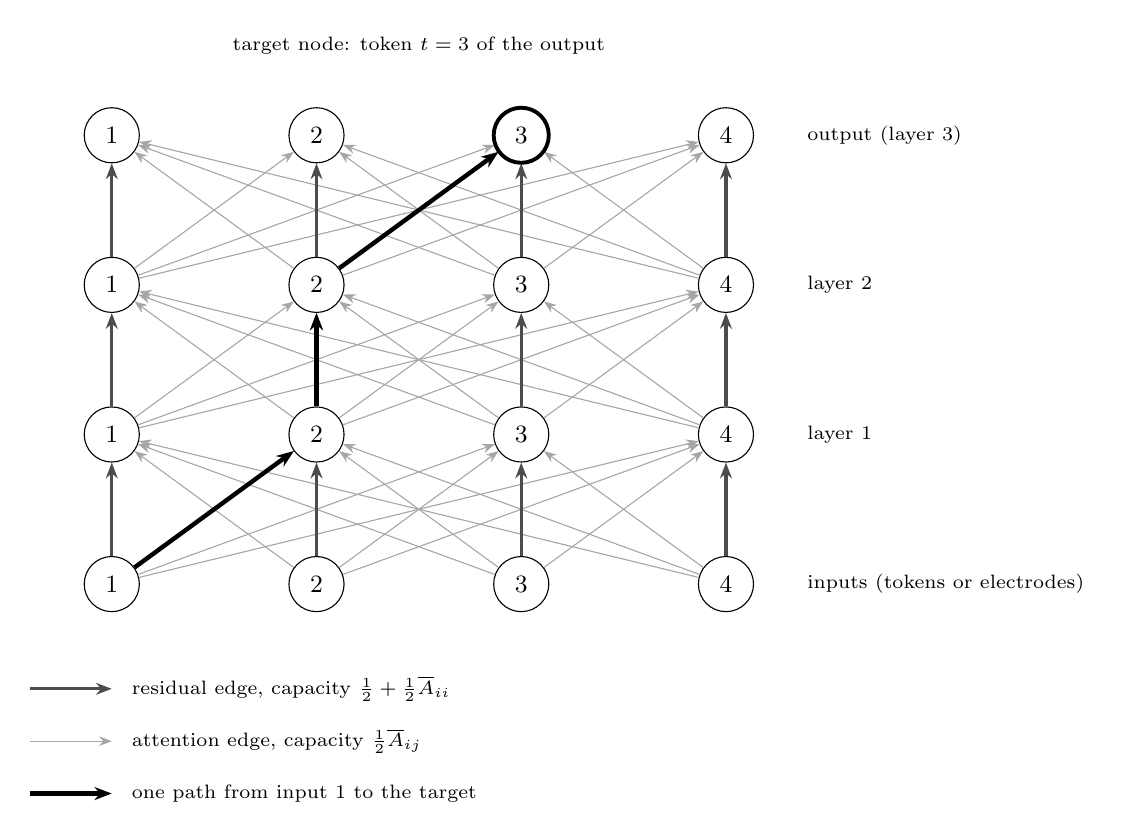
\begin{tikzpicture}[x=2.6cm, y=1.9cm, font=\footnotesize,
  nd/.style={circle, draw, minimum size=7mm, inner sep=0pt, font=\small, fill=white},
  att/.style={-{Stealth[length=1.6mm]}, black!35},
  res/.style={-{Stealth[length=2mm]}, line width=1.2pt, black!70},
  hot/.style={-{Stealth[length=2.2mm]}, line width=1.6pt, black}]
\foreach \l in {0,1,2,3}{\foreach \i in {1,2,3,4}{\node[nd] (n\l\i) at (\i,\l) {$\i$};}}
\foreach \l/\p in {1/0,2/1,3/2}{
  \foreach \i in {1,2,3,4}{\foreach \j in {1,2,3,4}{\ifnum\i=\j\else\draw[att] (n\p\j)--(n\l\i);\fi}}
  \foreach \i in {1,2,3,4}{\draw[res] (n\p\i)--(n\l\i);}
}
\draw[hot] (n01)--(n12); \draw[hot] (n12)--(n22); \draw[hot] (n22)--(n33);
\node[nd, line width=1.4pt] at (3,3) {$3$};
\foreach \l/\t in {0/{inputs (tokens or electrodes)},1/layer 1,2/layer 2,3/{output (layer 3)}}{\node[lab, anchor=west] at (4.35,\l) {\t};}
\node[lab] at (2.5,3.6) {target node: token $t=3$ of the output};
\draw[res] (0.6,-0.7)--(1.0,-0.7); \node[lab, anchor=west] at (1.05,-0.7) {residual edge, capacity $\tfrac12+\tfrac12\overline{A}_{ii}$};
\draw[att] (0.6,-1.05)--(1.0,-1.05); \node[lab, anchor=west] at (1.05,-1.05) {attention edge, capacity $\tfrac12\overline{A}_{ij}$};
\draw[hot] (0.6,-1.4)--(1.0,-1.4); \node[lab, anchor=west] at (1.05,-1.4) {one path from input 1 to the target};
\end{tikzpicture}
\end{latin}

\caption{\lr{layered graph} \lr{rollout} و \lr{attention flow}. وزن هر یال همان $\hat A_l[i,j]$ است. \lr{rollout} روی همه‌ی مسیرها از ورودی به هدف حاصل‌ضرب وزن‌ها را جمع می‌زند؛ \lr{attention flow} وزن‌ها را ظرفیت لوله می‌داند و بیشینه‌ی جریانی را که از یک ورودی به هدف می‌رسد حساب می‌کند.}
\label{fig:layered}
\end{figure}

\subsection{\lr{attention rollout}}

\subsubsection*{تعریف}
\lr{rollout} حاصل‌ضرب ماتریس‌های لایه‌ها از آخر به اول است، و این حاصل‌ضرب دقیقاً جمع روی همه‌ی مسیرهای \lr{layered graph} است:
\begin{equation}
R=\hat A_L\hat A_{L-1}\cdots\hat A_1,\qquad
R[t,\tau]=\sum_{\tau=i_0\to i_1\to\cdots\to i_L=t}\ \prod_{l=1}^{L}\hat A_l[i_l,i_{l-1}] .
\label{eq:rollout}
\end{equation}
هر مسیر به اندازه‌ی حاصل‌ضرب وزن‌هایش سهم می‌گیرد، پس یک یال ضعیف کل مسیر را تضعیف می‌کند. چون همه‌ی $\hat A_l$ سطرهایی با جمع ۱ و درایه‌های نامنفی دارند، حاصل‌ضرب آن‌ها هم همین‌طور است:
\begin{equation}
\hat A_l\mathbf 1=\mathbf 1\ \ \forall l\quad\Longrightarrow\quad R\,\mathbf 1=\hat A_L\cdots\hat A_1\mathbf 1=\mathbf 1,\qquad \sum_\tau R[t,\tau]=1 ,
\end{equation}
و سطر $t$ از $R$ یک توزیع روی ورودی‌هاست: سهم هر ورودی در خروجی \lr{token} $t$.

\subsubsection*{\lr{rollout} در هر مسیر مدل}
همین حاصل‌ضرب، مرحله به مرحله، برای هر خروجی:
\begin{itemize}
\item \textbf{\lr{K}، زمان} (سه لایه‌ی زمانی سینماتیک و \lr{stem}): $R_K=\hat A^{(k)}_3\hat A^{(k)}_2\hat A^{(k)}_1\,S$
\item \textbf{\lr{E}، زمان} (دو لایه‌ی زمانی \lr{EEG}): $R_E=\hat A^{(t)}_2\hat A^{(t)}_1$
\item \textbf{\lr{E}، الکترودها در \lr{token} $\tau$} (دو لایه‌ی گراف الکترود و \lr{pooling}): $e_\tau=\pi_\tau\,\hat A^{(e)}_2(\tau)\,\hat A^{(e)}_1(\tau)\in\mathbb{R}^{32}$
\item \textbf{\lr{E}، زمان در الکترود}: $M_E[\tau,e]=R_E[t,\tau]\;e_\tau[e]$
\item \textbf{$F_{eeg}$}: $R_F=c_t\,R_E$، که $c_t$ سطر $t$ \lr{cross-attention} است (بدون \lr{residual connection})
\item \textbf{\lr{muscle graph}} (دو لایه): $R_M=\hat A^{(m)}_2\hat A^{(m)}_1\in\mathbb{R}^{5\times5}$
\end{itemize}
$S$ ردپای \lr{convolutional stem} \lr{K} است: ماتریسی نواری با پهنای ۵ که وزن هر جابه‌جایی برابر انرژی هسته در آن جابه‌جایی است و سطرهایش جمع ۱ دارند. $\pi_\tau$ وزن‌های \lr{pooling} الکترودها در \lr{token} $\tau$ است (جمع ۱). چون همه‌ی عامل‌ها جمع سطری ۱ دارند، $\sum_{\tau,e}M_E[\tau,e]=1$ هم برقرار است.

\subsubsection*{نمایش}
\lr{token} خود رخداد و همسایه‌هایش (ردپای ۵ توکنی \lr{stem}) همیشه بیشترین سهم را از مسیر مستقیم می‌گیرند و بقیه‌ی نقشه را پنهان می‌کنند. شکل‌ها سهم آن‌ها را جداگانه می‌نویسند و منحنی سهم بقیه‌ی \lr{tokens} را نشان می‌دهند:
\begin{equation}
\mathrm{own}=\sum_{\tau\in\mathcal{O}}R[t,\tau],\qquad s(\tau)=\frac{R[t,\tau]}{1-\mathrm{own}}\quad(\tau\notin\mathcal{O}),
\end{equation}
که $\mathcal{O}$ پنج \lr{token} اطراف $t$ است. نقشه‌ی هر رخداد جداگانه ساخته و سپس روی رخدادها میانگین و \lr{SEM} گرفته می‌شود.

\subsubsection*{نسخه‌ی وزن‌دار با گرادیان}
در \lr{gradient-weighted rollout} (بخش~\ref{sec:interp}) فقط $\overline{A}_l$ در رابطه‌ی~\eqref{eq:ahat} با $\tilde A_l=\mathrm{rownorm}\big(\frac1H\sum_h(A^{h}_l\odot\partial y/\partial A^{h}_l)^{+}\big)$ عوض می‌شود و بقیه‌ی مراحل همین است؛ نتیجه برای هر عضله جداست.

\subsubsection*{محدودیت‌ها}
\lr{rollout} فقط وزن‌های توجه را می‌بیند و آنچه بردارهای مقدار حمل می‌کنند در آن نیست. لایه‌های بدون توجه (\lr{embedding}، \lr{feed-forward}، \lr{decoder}) در آن وارد نمی‌شوند، و وزن \lr{۰٫۵} \lr{residual connection} انتخاب ماست، نه چیزی که مدل آموخته باشد.

\begin{figure}[p]
\centering
% Attention rollout: the whole process in the style of a paper figure.
\begin{latin}\resizebox{\textwidth}{!}{%
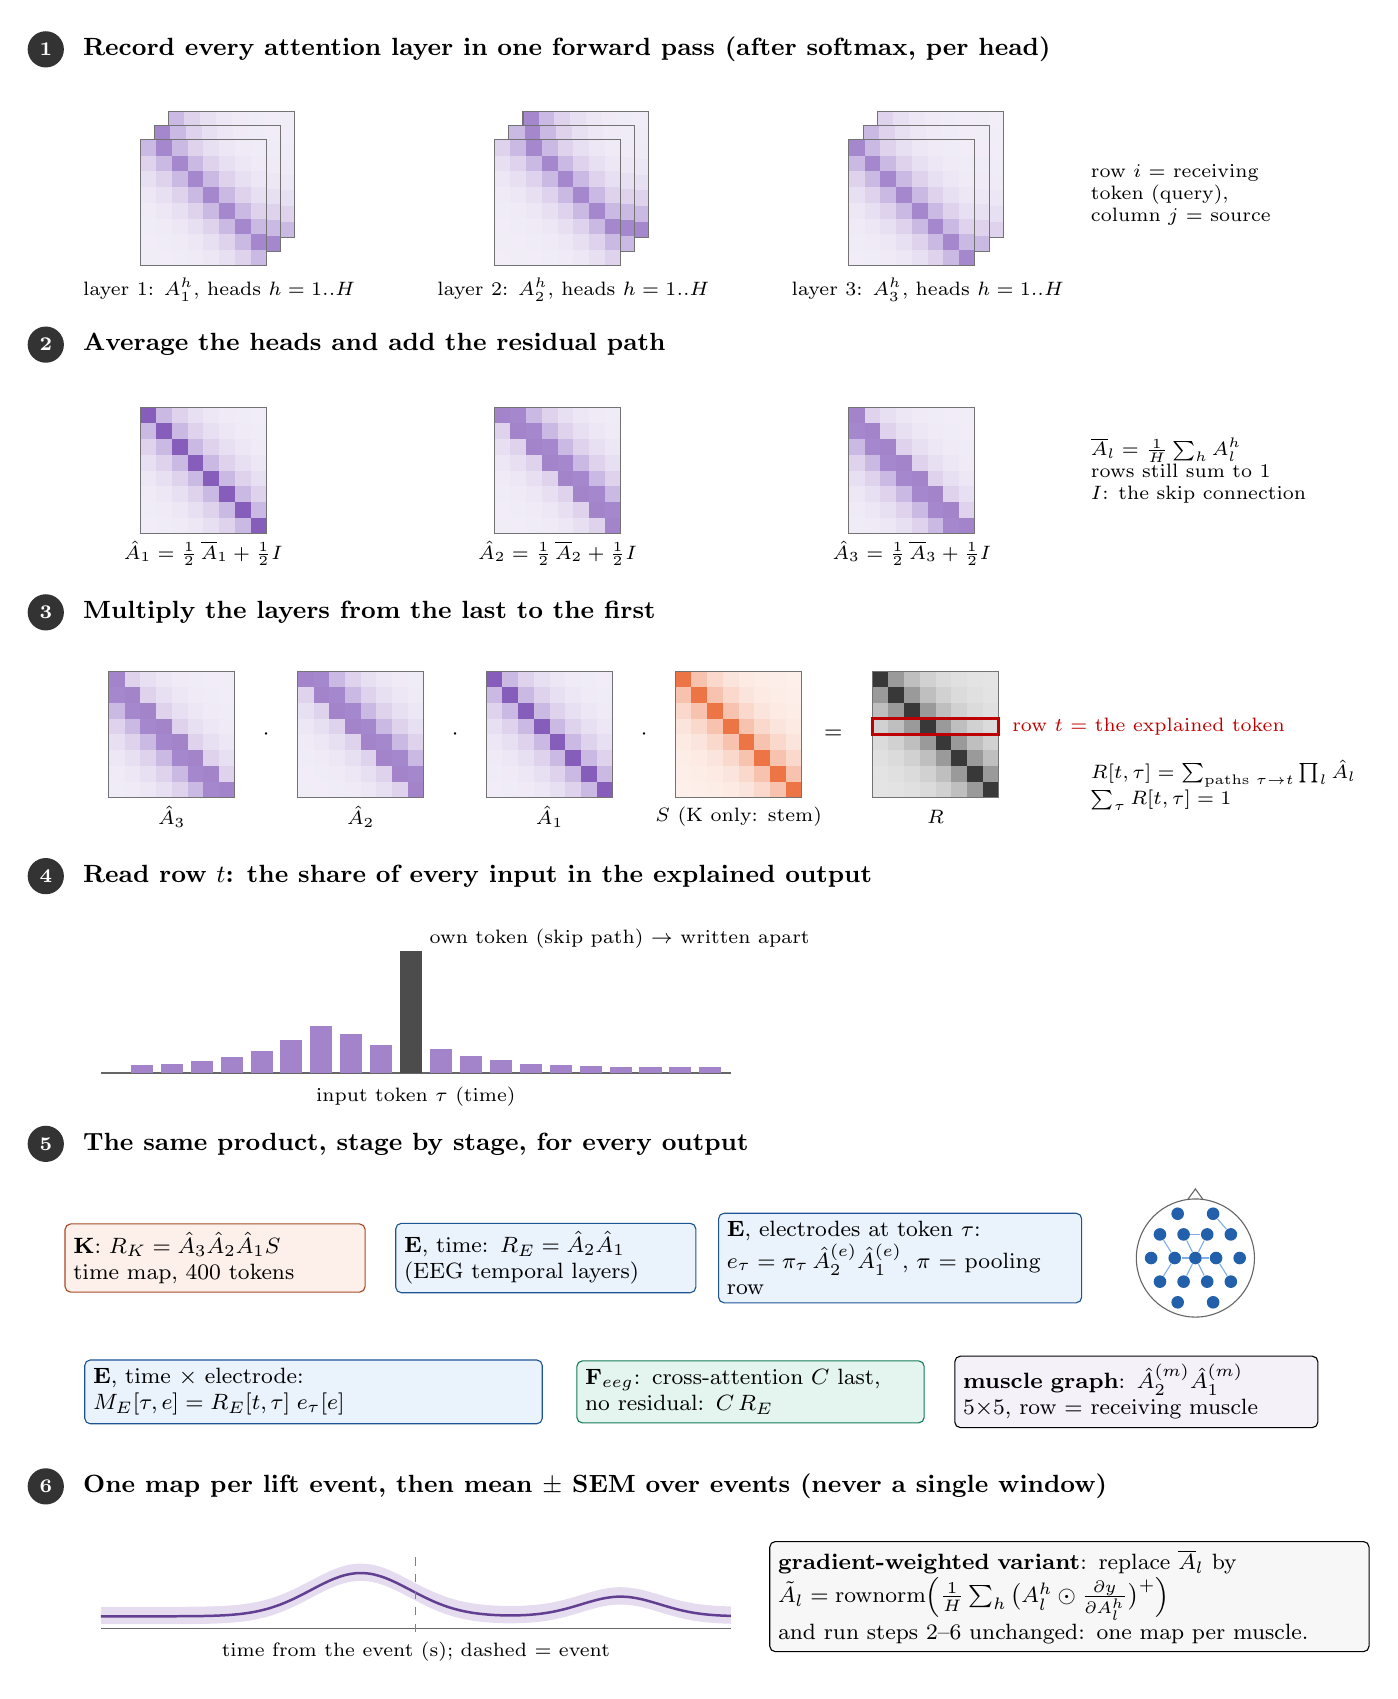
\begin{tikzpicture}[font=\footnotesize,
  stepc/.style={circle, fill=black!80, text=white, font=\scriptsize\bfseries, inner sep=1.2pt, minimum size=4.6mm},
  stitle/.style={lab, font=\small\bfseries, anchor=west}]
% ---------------- step 1: record
\node[stepc] at (-0.4,0.3) {1};
\node[stitle] at (-0.05,0.3) {Record every attention layer in one forward pass (after softmax, per head)};
\foreach \l/\x/\s in {1/1.6/0,2/6.1/-1,3/10.6/1}{
  \foreach \h in {2,1,0}{\attnmap{r1\l\h}{\x+0.18*\h,-1.65+0.18*\h}{8}{0.2}{\s+\h-1}{intc}{0}}
  \node[lab] at (\x+0.2,-2.75) {layer \l: $A^{h}_{\l}$, heads $h=1..H$};}
\node[lab, align=left, anchor=west] at (12.75,-1.55) {row $i$ = receiving\\ token (query),\\ column $j$ = source};

% ---------------- step 2: heads and residual
\node[stepc] at (-0.4,-3.45) {2};
\node[stitle] at (-0.05,-3.45) {Average the heads and add the residual path};
\foreach \l/\x/\s in {1/1.6/0,2/6.1/-1,3/10.6/1}{
  \attnmap{r2\l}{\x,-5.05}{8}{0.2}{\s}{intc}{30}
  \node[lab] at (\x,-6.1) {$\hat A_{\l}=\tfrac12\,\overline{A}_{\l}+\tfrac12 I$};
  }
\node[lab, align=left, anchor=west] at (12.75,-5.05) {$\overline{A}_l=\frac1H\sum_h A^{h}_l$\\ rows still sum to 1\\ $I$: the skip connection};

% ---------------- step 3: multiply
\node[stepc] at (-0.4,-6.85) {3};
\node[stitle] at (-0.05,-6.85) {Multiply the layers from the last to the first};
\attnmap{m3}{1.2,-8.4}{8}{0.2}{1}{intc}{30}\node[lab] at (1.2,-9.45) {$\hat A_3$};
\node at (2.4,-8.4) {$\cdot$};
\attnmap{m2}{3.6,-8.4}{8}{0.2}{-1}{intc}{30}\node[lab] at (3.6,-9.45) {$\hat A_2$};
\node at (4.8,-8.4) {$\cdot$};
\attnmap{m1}{6.0,-8.4}{8}{0.2}{0}{intc}{30}\node[lab] at (6.0,-9.45) {$\hat A_1$};
\node at (7.2,-8.4) {$\cdot$};
\attnmap{ms}{8.4,-8.4}{8}{0.2}{0}{kinc}{25}\node[lab] at (8.4,-9.45) {$S$ (K only: stem)};
\node at (9.6,-8.4) {$=$};
\attnmap{rr}{10.9,-8.4}{8}{0.2}{0}{black}{10}\node[lab] at (10.9,-9.45) {$R$};
\draw[red!75!black, line width=1pt] (10.1,-8.4+0.0) rectangle (11.7,-8.2);
\node[lab, text=red!75!black, anchor=west] at (11.75,-8.3) {row $t$ = the explained token};
\node[lab, align=left, anchor=west] at (12.75,-9.05) {$R[t,\tau]=\sum_{\text{paths }\tau\to t}\prod_l \hat A_l$\\ $\sum_\tau R[t,\tau]=1$};

% ---------------- step 4: read the row
\node[stepc] at (-0.4,-10.2) {4};
\node[stitle] at (-0.05,-10.2) {Read row $t$: the share of every input in the explained output};
\draw[black!60] (0.3,-12.7)--(8.3,-12.7);
\foreach \v [count=\k] in {0.10,0.12,0.15,0.2,0.28,0.42,0.6,0.5,0.35,1.55,0.3,0.22,0.16,0.12,0.1,0.09,0.08,0.08,0.07,0.07}{
  \fill[intc!70] (0.3+0.38*\k,-12.7) rectangle ++(0.28,\v);}
\fill[black!70] (0.3+0.38*10,-12.7) rectangle ++(0.28,1.55);
\node[lab, anchor=west] at (4.35,-11.0) {own token (skip path) $\to$ written apart};
\node[lab] at (4.3,-13.0) {input token $\tau$ (time)};

% ---------------- step 5: what R means in each stream
\node[stepc] at (-0.4,-13.6) {5};
\node[stitle] at (-0.05,-13.6) {The same product, stage by stage, for every output};
\node[kbox, text width=3.6cm, align=left] (b1) at (1.75,-15.05) {\textbf{K}: $R_K=\hat A_3\hat A_2\hat A_1 S$\\ time map, 400 tokens};
\node[ebox, text width=3.6cm, align=left] (b2) at (5.95,-15.05) {\textbf{E}, time: $R_E=\hat A_2\hat A_1$\\ (EEG temporal layers)};
\node[ebox, text width=4.4cm, align=left] (b3) at (10.45,-15.05) {\textbf{E}, electrodes at token $\tau$:\\ \mbox{$e_\tau=\pi_\tau\,\hat A^{(e)}_2\hat A^{(e)}_1$}, $\pi$ = pooling row};
\headgraph{hr}{14.2,-15.05}{0.75}
\node[ebox, text width=5.6cm, align=left] (b4) at (3.0,-16.75) {\textbf{E}, time $\times$ electrode:\\ $M_E[\tau,e]=R_E[t,\tau]\;e_\tau[e]$};
\node[fbox, text width=4.2cm, align=left] (b5) at (8.55,-16.75) {\textbf{F$_{eeg}$}: cross-attention $C$ last,\\ no residual: $C\,R_E$};
\node[box, fill=intc!8, text width=4.4cm, align=left] (b6) at (13.45,-16.75) {\textbf{muscle graph}: $\hat A^{(m)}_2\hat A^{(m)}_1$\\ 5$\times$5, row = receiving muscle};

% ---------------- step 6: average over events
\node[stepc] at (-0.4,-17.95) {6};
\node[stitle] at (-0.05,-17.95) {One map per lift event, then mean $\pm$ SEM over events (never a single window)};
\fill[intc!20] plot[smooth, domain=0.3:8.3, samples=50] (\x,{-19.6+0.55*exp(-((\x-3.6)^2)/0.8)+0.25*exp(-((\x-6.9)^2)/0.5)+0.12}) -- (8.3,-19.75) -- plot[smooth, domain=8.3:0.3, samples=50] (\x,{-19.75+0.55*exp(-((\x-3.6)^2)/0.8)+0.25*exp(-((\x-6.9)^2)/0.5)+0.05}) -- cycle;
\draw[intc!80!black, line width=0.9pt] plot[smooth, domain=0.3:8.3, samples=50] (\x,{-19.68+0.55*exp(-((\x-3.6)^2)/0.8)+0.25*exp(-((\x-6.9)^2)/0.5)+0.08});
\draw[black!60] (0.3,-19.75)--(8.3,-19.75); \draw[black!50, dashed] (4.3,-19.8)--(4.3,-18.75);
\node[lab] at (4.3,-20.05) {time from the event (s); dashed = event};
\node[box, fill=black!3, text width=7.4cm, align=left] at (12.6,-19.35) {\textbf{gradient-weighted variant}: replace $\overline{A}_l$ by\\ $\tilde A_l=\mathrm{rownorm}\Big(\frac1H\sum_h\big(A^{h}_l\odot\frac{\partial y}{\partial A^{h}_l}\big)^{+}\Big)$\\ and run steps 2--6 unchanged: one map per muscle.};
\end{tikzpicture}}\end{latin}

\caption{فرایند کامل \lr{attention rollout}. (۱) \lr{recorder} توجه هر لایه و هر سر را در یک گذر برمی‌دارد. (۲) سرها میانگین گرفته و \lr{residual connection} به‌صورت $\tfrac12 I$ اضافه می‌شود. (۳) ماتریس‌ها از لایه‌ی آخر به اول ضرب می‌شوند (برای \lr{K} ردپای \lr{stem} $S$ هم). (۴) سطر \lr{token} توضیح‌داده‌شده سهم هر ورودی است؛ سهم \lr{token} خود رخداد جداگانه نوشته می‌شود. (۵) همین حاصل‌ضرب برای زمان، الکترودها، زمان در الکترود، اصلاح \lr{EEG} و \lr{muscle graph}. (۶) نقشه‌ی هر رخداد ساخته و روی رخدادها میانگین گرفته می‌شود. کادر پایین: نسخه‌ی وزن‌دار با گرادیان.}
\label{fig:rollout-process}
\end{figure}

\subsection{\lr{attention flow}}

\subsubsection*{تعریف}
در \lr{attention flow} هر یال \lr{layered graph} یک لوله با ظرفیت $c_e=\hat A_l[i,j]$ است. برای ورودی (منبع) $\tau$ و گره هدف $t$، جریان یک تابع $f$ روی یال‌هاست و بیشینه‌ی مقدار آن جواب است:
\begin{equation}
\mathrm{flow}(\tau\to t)=\max_{f}\ \sum_{e\,\in\,\mathrm{out}(\tau)} f_e
\quad\text{که}\quad 0\le f_e\le c_e,\qquad \sum_{e\,\in\,\mathrm{in}(v)}f_e=\sum_{e\,\in\,\mathrm{out}(v)}f_e\ \ \text{برای هر گره میانی }v .
\label{eq:flow}
\end{equation}
طبق قضیه‌ی \lr{maximum flow} و \lr{minimum cut}، این مقدار برابر ظرفیت کم‌هزینه‌ترین برشی است که $\tau$ را از $t$ جدا می‌کند:
\begin{equation}
\mathrm{flow}(\tau\to t)=\min_{(\mathcal{S},\mathcal{T}):\ \tau\in\mathcal{S},\ t\in\mathcal{T}}\ \sum_{e:\,\mathcal{S}\to\mathcal{T}}c_e .
\end{equation}
فرق با \lr{rollout}: \lr{rollout} در طول هر مسیر ضرب می‌کند، اما جریان مسیرهای موازی را جمع می‌کند و هر مسیر فقط با باریک‌ترین لوله‌اش محدود می‌شود. به همین دلیل جریان هیچ‌گاه از سهم \lr{rollout} کمتر نیست و وقتی توجه پخش است، زود به سقف می‌رسد.

\subsubsection*{بازه‌بندی زمان}
حل رابطه‌ی~\eqref{eq:flow} روی ۴۰۰ \lr{tokens} برای هر منبع بسیار پرهزینه است. زمان به بازه‌های ۴ توکنی (۸۰ میلی‌ثانیه) تقسیم می‌شود: سطرهای گیرنده‌ی هر بازه میانگین و ستون‌های فرستنده جمع می‌شوند،
\begin{equation}
\hat A^{bin}_l[a,b]=\frac{1}{|a|}\sum_{i\in a}\sum_{j\in b}\hat A_l[i,j],
\end{equation}
که سطرها را همچنان با جمع ۱ نگه می‌دارد. برای \lr{K} ماتریس \lr{stem} $S$ هم با همین قاعده بازه‌بندی و پیش از لایه‌ی اول گذاشته می‌شود؛ برای $F_{eeg}$ سطر \lr{cross-attention} لایه‌ی آخر است.

\subsubsection*{جریان الکترودها}
برای \lr{E} و $F_{eeg}$، در هر بازه‌ی زمانی $\tau$ گراف دیگری هست: دو لایه‌ی \lr{electrode graph} ($32\to32\to32$، با \lr{residual connection}) و ردیف \lr{pooling} ($32\to1$ با ظرفیت $\pi_\tau[e]$ و بدون \lr{residual connection}). $\mathrm{flow}_{elec}(\tau,e)$ \lr{maximum flow} از الکترود $e$ تا \lr{token} پول‌شده است. چون \lr{token} پول‌شده تنها راه خروج اطلاعات الکترودهای یک گام زمانی است، جریان یک الکترود در یک زمان تا خروجی کمینه‌ی دو مرحله است:
\begin{equation}
\mathrm{flow}(\tau,e)=\min\big(\mathrm{flow}_{time}(\tau),\ \mathrm{flow}_{elec}(\tau,e)\big).
\end{equation}

\subsubsection*{خط پایه‌ی توجه یکنواخت}
همان محاسبه برای مدلی تکرار می‌شود که در هر لایه به همه‌ی $n$ موقعیت برابر توجه می‌کند، با همان \lr{residual connection} و همان \lr{stem}:
\begin{equation}
\hat A^{u}=\tfrac12\cdot\tfrac1n J+\tfrac12 I,\qquad \mathrm{excess}(\tau)=\mathrm{flow}(\tau)-\mathrm{flow}^{u}(\tau),
\end{equation}
که $J$ ماتریس تمام‌یک است. فقط $\mathrm{excess}$ به الگوی توجه آموخته‌شده مربوط است؛ $\mathrm{flow}^{u}$ چیزی است که حتی یک مدل آموزش‌ندیده هم می‌دهد.

\begin{figure}[p]
\centering
% Attention flow: the whole process in the style of a paper figure.
\begin{latin}\resizebox{\textwidth}{!}{%
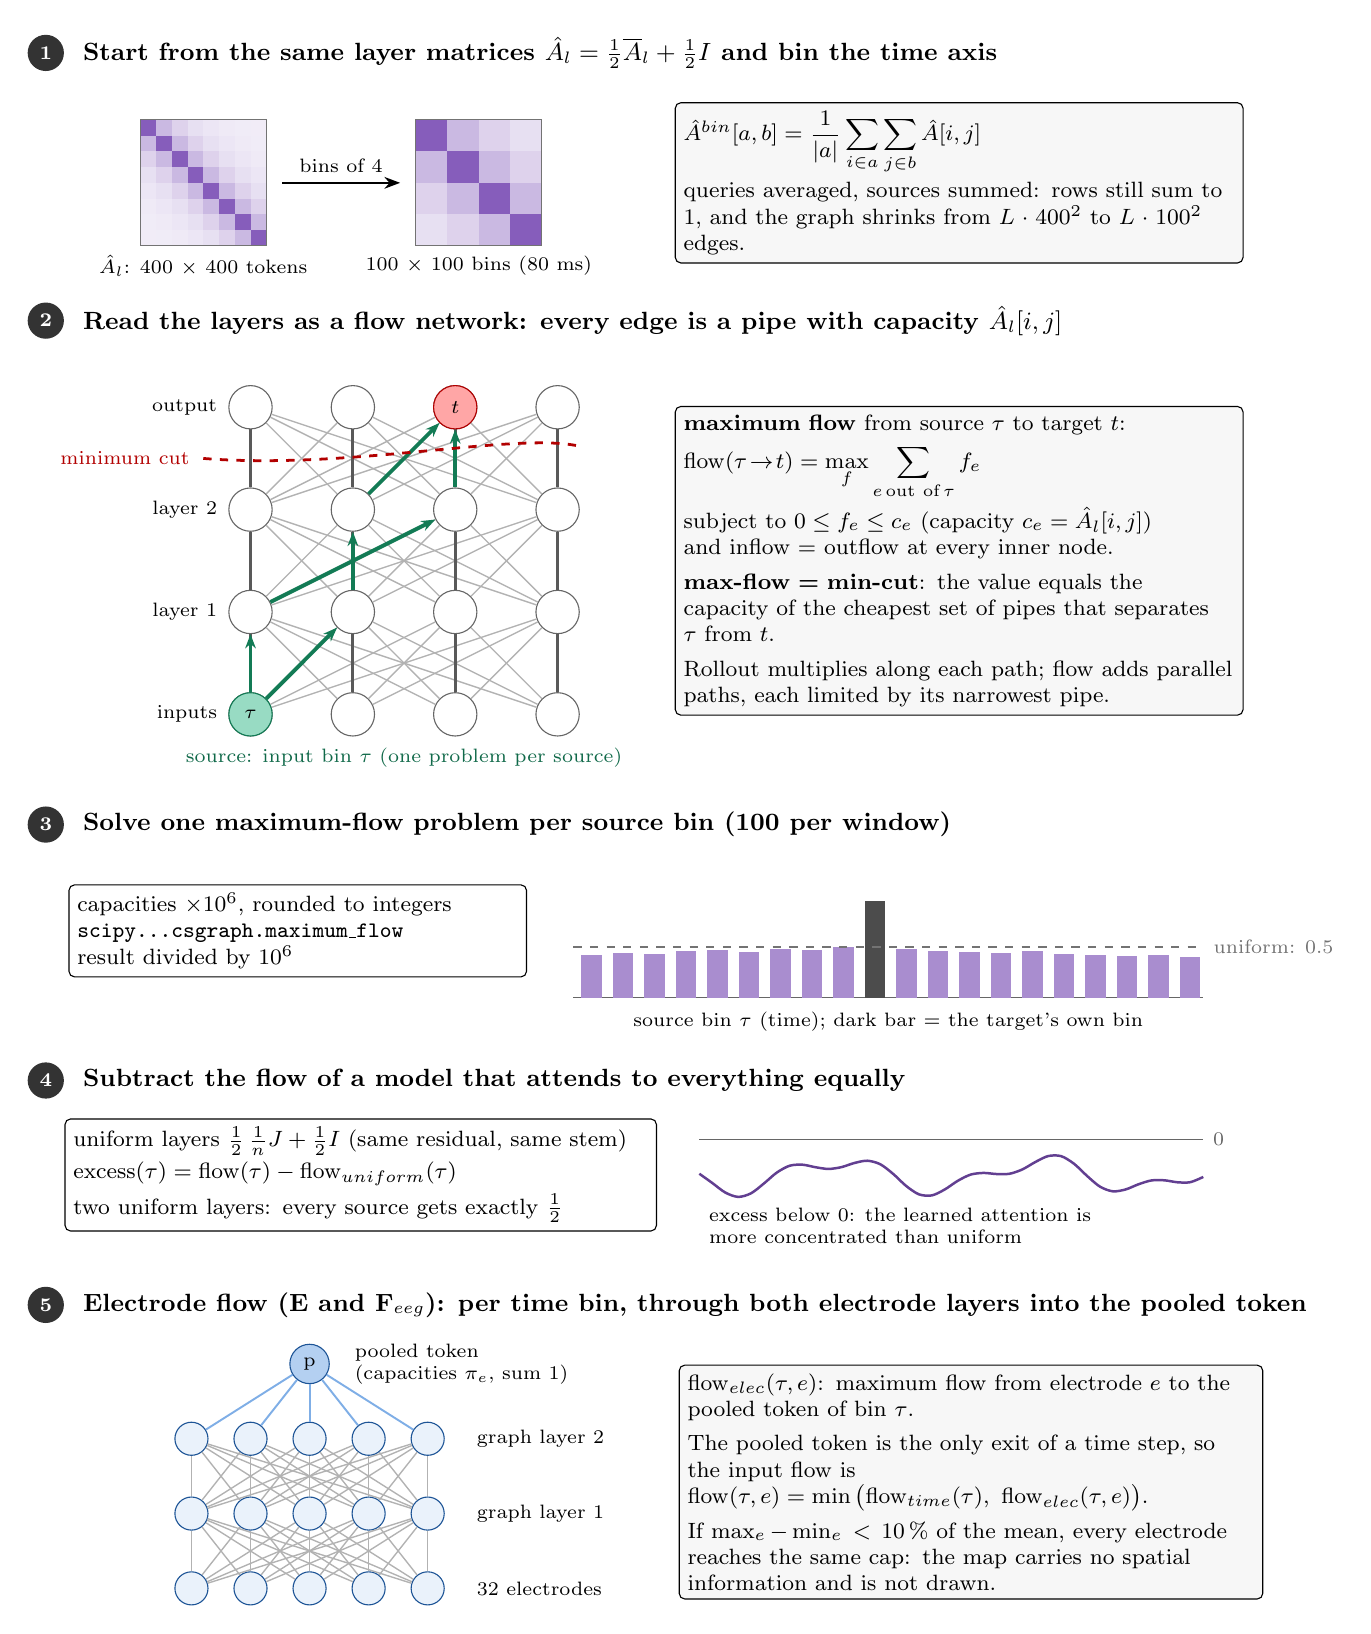
\begin{tikzpicture}[font=\footnotesize,
  stepc/.style={circle, fill=black!80, text=white, font=\scriptsize\bfseries, inner sep=1.2pt, minimum size=4.6mm},
  stitle/.style={lab, font=\small\bfseries, anchor=west},
  fn/.style={circle, draw=black!60, fill=white, minimum size=5.5mm, inner sep=0pt, font=\scriptsize},
  capedge/.style={black!30, line width=0.5pt},
  resedge/.style={black!65, line width=1.1pt},
  fl/.style={-{Stealth[length=1.8mm]}, fusc!70!black, line width=1.4pt}]
% ---------------- step 1: same matrices, binned
\node[stepc] at (-0.4,0.3) {1};
\node[stitle] at (-0.05,0.3) {Start from the same layer matrices $\hat A_l=\tfrac12\overline{A}_l+\tfrac12I$ and bin the time axis};
\attnmap{f1}{1.6,-1.35}{8}{0.2}{0}{intc}{30}
\node[lab] at (1.6,-2.4) {$\hat A_l$: 400 $\times$ 400 tokens};
\draw[arr] (2.6,-1.35)--(4.1,-1.35) node[lab, midway, above]{bins of 4};
\attnmap{f2}{5.1,-1.35}{4}{0.4}{0}{intc}{30}
\node[lab] at (5.1,-2.4) {100 $\times$ 100 bins (80 ms)};
\node[box, fill=black!3, text width=7.0cm, align=left] at (11.2,-1.35) {$\hat A^{bin}[a,b]=\dfrac{1}{|a|}\displaystyle\sum_{i\in a}\sum_{j\in b}\hat A[i,j]$\\[2pt] queries averaged, sources summed: rows still sum to 1, and the graph shrinks from $L\cdot400^2$ to $L\cdot100^2$ edges.};

% ---------------- step 2: the flow network
\node[stepc] at (-0.4,-3.1) {2};
\node[stitle] at (-0.05,-3.1) {Read the layers as a flow network: every edge is a pipe with capacity $\hat A_l[i,j]$};
\foreach \l in {0,1,2,3}{\foreach \i in {1,2,3,4}{\node[fn] (g\l\i) at (0.9+1.3*\i,-8.1+1.3*\l) {};}}
\foreach \l/\p in {1/0,2/1,3/2}{
  \foreach \i in {1,2,3,4}{\foreach \j in {1,2,3,4}{\ifnum\i=\j\else\draw[capedge] (g\p\j)--(g\l\i);\fi}}
  \foreach \i in {1,2,3,4}{\draw[resedge] (g\p\i)--(g\l\i);}}
\node[fn, fill=fusc!45, draw=fusc!70!black] at (g01) {$\tau$};
\node[fn, fill=red!35, draw=red!70!black] at (g33) {$t$};
\draw[fl] (g01)--(g12); \draw[fl] (g12)--(g22); \draw[fl] (g22)--(g33);
\draw[fl] (g01)--(g11); \draw[fl] (g11)--(g23); \draw[fl] (g23)--(g33);
\draw[red!70!black, dashed, line width=1pt] (1.6,-4.85)..controls (3.5,-5.0) and (5.6,-4.5)..(6.4,-4.7);
\node[lab, text=red!70!black, anchor=east] at (1.55,-4.85) {minimum cut};
\node[lab, anchor=east] at (1.9,-8.1) {inputs}; \node[lab, anchor=east] at (1.9,-6.8) {layer 1};
\node[lab, anchor=east] at (1.9,-5.5) {layer 2}; \node[lab, anchor=east] at (1.9,-4.2) {output};
\node[lab, text=fusc!60!black] at (4.15,-8.65) {source: input bin $\tau$ (one problem per source)};
\node[box, fill=black!3, text width=7.0cm, align=left] at (11.2,-6.15) {\textbf{maximum flow} from source $\tau$ to target $t$:\\[3pt]
 $\displaystyle\mathrm{flow}(\tau\!\to\!t)=\max_{f}\sum_{e\,\text{out of}\,\tau} f_e$\\[2pt]
 subject to $0\le f_e\le c_e$ (capacity $c_e=\hat A_l[i,j]$)\\ and inflow = outflow at every inner node.\\[3pt]
 \textbf{max-flow = min-cut}: the value equals the capacity of the cheapest set of pipes that separates $\tau$ from $t$.\\[3pt]
 Rollout multiplies along each path; flow adds parallel paths, each limited by its narrowest pipe.};

% ---------------- step 3: solve
\node[stepc] at (-0.4,-9.5) {3};
\node[stitle] at (-0.05,-9.5) {Solve one maximum-flow problem per source bin (100 per window)};
\node[box, text width=5.6cm, align=left] at (2.8,-10.85) {capacities $\times 10^{6}$, rounded to integers\\ \texttt{scipy...csgraph.maximum\_flow}\\ result divided by $10^{6}$};
\draw[black!60] (6.3,-11.7)--(14.3,-11.7);
\foreach \v [count=\k] in {0.42,0.44,0.43,0.46,0.47,0.45,0.48,0.47,0.5,0.95,0.48,0.46,0.45,0.44,0.46,0.43,0.42,0.41,0.42,0.4}{
  \fill[intc!65] (6.3+0.4*\k-0.3,-11.7) rectangle ++(0.26,\v*1.3);}
\fill[black!70] (6.3+0.4*10-0.3,-11.7) rectangle ++(0.26,0.95*1.3);
\draw[black!55, dashed, line width=0.8pt] (6.3,-11.7+0.5*1.3)--(14.3,-11.7+0.5*1.3) node[lab, anchor=west]{uniform: 0.5};
\node[lab] at (10.3,-12.0) {source bin $\tau$ (time); dark bar = the target's own bin};

% ---------------- step 4: baseline
\node[stepc] at (-0.4,-12.75) {4};
\node[stitle] at (-0.05,-12.75) {Subtract the flow of a model that attends to everything equally};
\node[box, text width=7.3cm, align=left] at (3.6,-13.95) {uniform layers $\tfrac12\,\tfrac1n J+\tfrac12 I$ (same residual, same stem)\\[2pt] $\mathrm{excess}(\tau)=\mathrm{flow}(\tau)-\mathrm{flow}_{uniform}(\tau)$\\[2pt] two uniform layers: every source gets exactly $\tfrac12$};
\draw[black!60] (7.9,-13.5)--(14.3,-13.5) node[lab, anchor=west]{0};
\draw[intc!80!black, line width=0.9pt] plot[smooth, domain=7.9:14.3, samples=40] (\x,{-13.5-0.45-0.18*sin(\x*140)-0.1*sin(\x*310)});
\node[lab, anchor=west, align=left] at (7.9,-14.6) {excess below 0: the learned attention is\\ more concentrated than uniform};

% ---------------- step 5: electrodes
\node[stepc] at (-0.4,-15.6) {5};
\node[stitle] at (-0.05,-15.6) {Electrode flow (E and F$_{eeg}$): per time bin, through both electrode layers into the pooled token};
\foreach \l in {0,1,2}{\foreach \i in {1,...,5}{\node[fn, minimum size=4.2mm, fill=eegc!10, draw=eegc!70!black] (e\l\i) at (0.7+0.75*\i,-19.2+0.95*\l) {};}}
\node[fn, minimum size=5mm, fill=eegc!35, draw=eegc!70!black] (pool) at (2.95,-16.35) {p};
\foreach \l/\p in {1/0,2/1}{\foreach \i in {1,...,5}{\foreach \j in {1,...,5}{\draw[capedge] (e\p\j)--(e\l\i);}}}
\foreach \i in {1,...,5}{\draw[eegc!60, line width=0.7pt] (e2\i)--(pool);}
\node[lab, anchor=west] at (4.95,-19.2) {32 electrodes};
\node[lab, anchor=west] at (4.95,-18.25) {graph layer 1};
\node[lab, anchor=west] at (4.95,-17.3) {graph layer 2};
\node[lab, anchor=west, align=left] at (3.4,-16.35) {pooled token\\ (capacities $\pi_e$, sum 1)};
\node[box, fill=black!3, text width=7.2cm, align=left] at (11.35,-17.85) {$\mathrm{flow}_{elec}(\tau,e)$: maximum flow from electrode $e$ to the pooled token of bin $\tau$.\\[3pt]
 The pooled token is the only exit of a time step, so the input flow is\\ $\mathrm{flow}(\tau,e)=\min\big(\mathrm{flow}_{time}(\tau),\ \mathrm{flow}_{elec}(\tau,e)\big)$.\\[3pt]
 If $\max_e-\min_e<10\,\%$ of the mean, every electrode reaches the same cap: the map carries no spatial information and is not drawn.};
\end{tikzpicture}}\end{latin}

\caption{فرایند کامل \lr{attention flow}. (۱) همان ماتریس‌های لایه‌ها، با بازه‌بندی زمان به ۱۰۰ بازه‌ی ۸۰ میلی‌ثانیه‌ای. (۲) لایه‌ها به‌صورت شبکه‌ی جریان خوانده می‌شوند: هر یال لوله‌ای با ظرفیت $\hat A_l[i,j]$ است؛ \lr{maximum flow} از منبع $\tau$ تا هدف $t$ برابر ظرفیت \lr{minimum cut} است. (۳) برای هر بازه‌ی منبع یک مسئله‌ی \lr{maximum flow} با ظرفیت‌های صحیح حل می‌شود. (۴) جریان یک مدل با توجه یکنواخت کم می‌شود؛ مقدار زیر صفر یعنی توجه آموخته‌شده متمرکزتر از یکنواخت است. (۵) جریان الکترودها از دو لایه‌ی گراف الکترود و \lr{pooling} عبور می‌کند و جریان ورودی کمینه‌ی جریان زمانی و جریان الکترود است.}
\label{fig:flow-process}
\end{figure}

\subsection{پیاده‌سازی}

تابع \lr{trace} مدل را یک بار با \lr{recorder} اجرا می‌کند و برای هر لایه تنسور $(B,H,n,n)$ را برمی‌دارد. \lr{layer\_matrix} رابطه‌ی~\eqref{eq:ahat} را می‌سازد و \lr{rollout} ماتریس‌ها را به ترتیب از لایه‌ی آخر به اول ضرب می‌کند. \lr{rollout} با تابع \lr{rollout} مدل پایه روی ماتریس‌های دست‌ساز آزموده شده است.

برای جریان، \lr{bin\_matrix} بازه‌بندی را انجام می‌دهد و \lr{attention\_flow} برای هر منبع یک مسئله‌ی \lr{maximum flow} با \lr{SciPy} حل می‌کند. این الگوریتم ظرفیت صحیح می‌خواهد، پس ظرفیت‌ها در $10^{6}$ ضرب و گرد می‌شوند و جواب دوباره بر $10^{6}$ تقسیم می‌شود. هر پنجره ۱۰۰ مسئله دارد، پس جریان برای هر خروجی و هر نوع رخداد فقط روی حداکثر ۶ رخداد حساب می‌شود. جریان با \lr{maximum flow} دست‌حساب‌شده روی گلوگاه‌های ساده آزموده شده و هیچ‌گاه کمتر از \lr{rollout} نیست.

\begin{figure}[htbp]
\centering
% Implementation of rollout (left) and attention flow (right) on the time path.
\begin{latin}
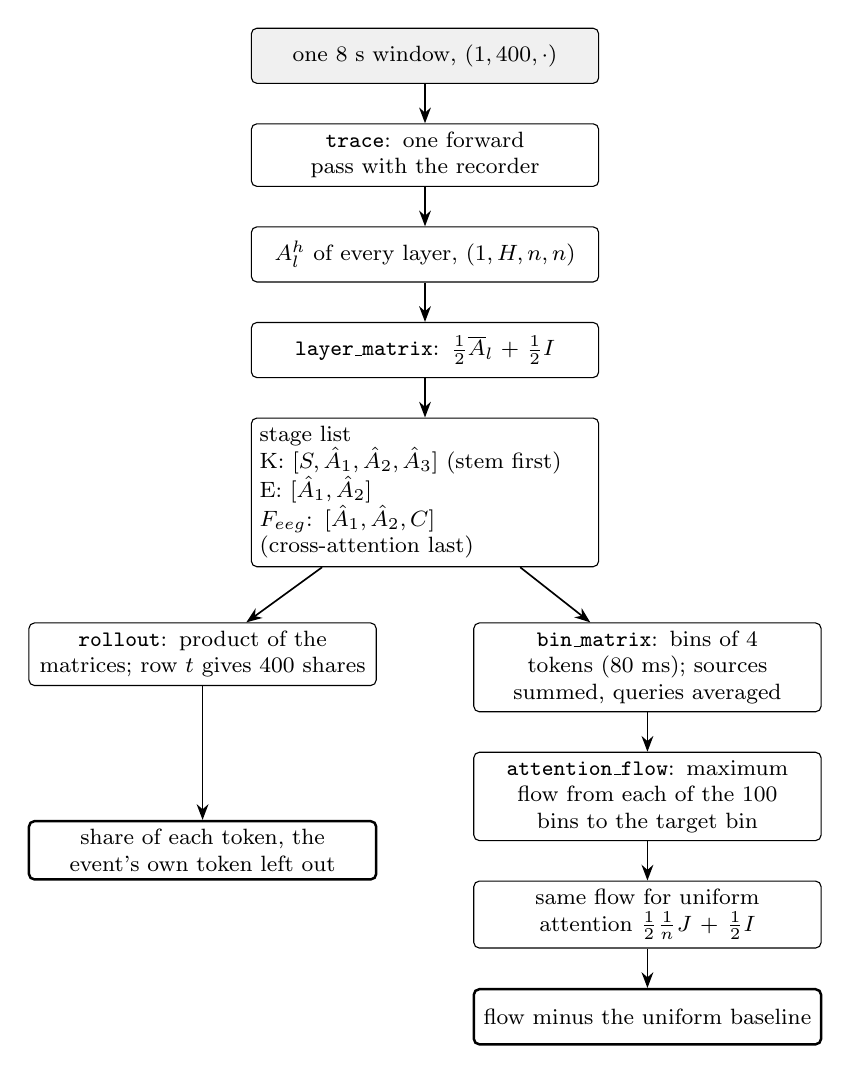
\begin{tikzpicture}[node distance=5mm and 5mm, font=\footnotesize, box/.append style={text width=4.2cm}]
\node[io] (x) {one 8 s window, $(1,400,\cdot)$};
\node[box, below=of x] (tr) {\texttt{trace}: one forward pass with the recorder};
\node[box, below=of tr] (A) {$A^{h}_l$ of every layer, $(1,H,n,n)$};
\node[box, below=of A] (L) {\texttt{layer\_matrix}: $\tfrac12\overline{A}_l+\tfrac12I$};
\node[box, below=of L, align=left] (st) {stage list\\ K: $[S,\hat A_1,\hat A_2,\hat A_3]$ (stem first)\\ E: $[\hat A_1,\hat A_2]$\\ $F_{eeg}$: $[\hat A_1,\hat A_2,C]$ (cross-attention last)};
\node[box, below left=7mm and -16mm of st] (ro) {\texttt{rollout}: product of the matrices; row $t$ gives 400 shares};
\node[box, below right=7mm and -16mm of st] (bn) {\texttt{bin\_matrix}: bins of 4 tokens (80 ms); sources summed, queries averaged};
\node[box, below=of bn] (fl) {\texttt{attention\_flow}: maximum flow from each of the 100 bins to the target bin};
\node[box, below=of fl] (un) {same flow for uniform attention $\tfrac12\frac1n J+\tfrac12 I$};
\node[result, below=of un] (ex) {flow minus the uniform baseline};
\node[result, below=17mm of ro] (rs) {share of each token, the event's own token left out};
\draw[arr] (x)--(tr); \draw[arr] (tr)--(A); \draw[arr] (A)--(L); \draw[arr] (L)--(st);
\draw[arr] (st)--(ro); \draw[arr] (st)--(bn); \draw[arr] (bn)--(fl); \draw[arr] (fl)--(un); \draw[arr] (un)--(ex); \draw[arr] (ro)--(rs);
\end{tikzpicture}
\end{latin}

\caption{پیاده‌سازی \lr{rollout} (چپ) و \lr{attention flow} (راست) برای مسیر زمانی.}
\label{fig:rf-impl}
\end{figure}

\subsection{چرا \lr{attention flow} در این مدل اشباع می‌شود}

مثال دو لایه با توجه یکنواخت روی $n$ موقعیت را در نظر بگیرید (مسیر زمانی \lr{E}). ظرفیت یال از ورودی $j$ به گره میانی $i$ برابر $\tfrac{1}{2n}+\tfrac12\delta_{ij}$ و از $i$ به هدف $t$ برابر $\tfrac{1}{2n}+\tfrac12\delta_{it}$ است. برای $j\ne t$ مسیرها از گره‌های میانی جدا می‌گذرند و هر کدام با کوچک‌ترین یال خود محدود می‌شوند:
\begin{equation}
\mathrm{flow}(j\to t)=\sum_{i=1}^{n}\min\!\Big(\tfrac{1}{2n}+\tfrac12\delta_{ij},\ \tfrac{1}{2n}+\tfrac12\delta_{it}\Big)=n\cdot\tfrac{1}{2n}=\tfrac12,
\end{equation}
و برای خود هدف ($j=t$) نزدیک به ۱. پس در مدلی که هیچ چیز نیاموخته، همه‌ی ورودی‌ها جریان \lr{۰٫۵} دارند و جریان در \lr{token} خود رخداد به ۱ می‌پرد. با \lr{stem} و سه لایه (مسیر \lr{K}) این عدد برای همه‌ی ورودی‌ها حدود ۱ است. وقتی توجه پخش است، تعداد زیاد مسیرهای موازی کوچک جمع می‌شود و جریان به «پخش بودن توجه» حساس است، نه به اینکه اطلاعات از کجا آمده است.

در الکترودها وضع بدتر است. جریان هر الکترود باید از ردیف \lr{pooling} بگذرد که ظرفیت کل آن ۱ است، و ظرفیت خروجی هر الکترود در لایه‌ی اول دست‌کم \lr{۰٫۵} است. با توجه نسبتاً پخش در لایه‌ی دوم، تقریباً همه‌ی الکترودها به یک سقف می‌رسند: در \lr{P1} سهم جریان همه‌ی ۳۲ الکترود بین \lr{۳٫۰۹} و \lr{۳٫۱۵} درصد است (سهم یکنواخت \lr{۳٫۱۲۵} درصد است). شکل‌ها در این حالت نقشه‌ی جریان الکترود را رسم نمی‌کنند و دلیلش را در عنوان می‌نویسند.

\subsection{نتایج}

جدول~\ref{tab:flow} و شکل~\ref{fig:flow_all.png} جریان را در برابر خط پایه برای هر ۱۲ شرکت‌کننده نشان می‌دهند. سه نتیجه:
\begin{enumerate}
\item جریان واقعی همه‌جا \emph{کمتر} از \lr{uniform-attention flow} است (میانگین \lr{−۰٫۱۵} برای \lr{K}، \lr{−۰٫۲۱} برای \lr{E} و \lr{−۰٫۲۴} برای $F_{eeg}$). یعنی توجه آموخته‌شده متمرکزتر از یکنواخت است و راه بسیاری از ورودی‌ها را می‌بندد.
\item برای \lr{K} الگوی زمانی در همه‌ی شرکت‌کننده‌ها یکسان است: ورودی‌های ۰ تا ۳ ثانیه پس از جداشدن کمترین جریان را دارند و ورودی‌های پیش از رخداد بیشترین. این با \lr{rollout} سازگار است: \lr{K} برای سطح فعالیت در لحظه‌ی جداشدن، به حرکت پیش از آن نگاه می‌کند.
\item پراکندگی جریان الکترودها در ۱۰ نفر از ۱۲ کمتر از ۱۰ درصد میانگین است؛ فقط \lr{P2} (۱۲ درصد) از این مرز می‌گذرد. جریان الکترود در این مدل تقریباً هیچ اطلاعات مکانی ندارد.
\end{enumerate}
در \lr{deletion check} (جدول~\ref{tab:interp-del}) جریان برای \lr{K} ضعیف‌ترین روش است (\lr{۰٫۱۱۸} در برابر حدود \lr{۰٫۲۱}) و برای \lr{E} هم‌تراز \lr{plain rollout} و بسیار ضعیف‌تر از \lr{gradient-weighted rollout}. نتیجه‌ی عملی: \lr{attention flow} در این معماری درست محاسبه می‌شود اما برای مکان‌یابی اطلاعات به کار نمی‌آید؛ \lr{gradient-weighted rollout} روش اصلی است و جریان فقط به‌صورت «فاصله از خط پایه‌ی یکنواخت» گزارش می‌شود.

\begin{table}[htbp]
\centering
\small
\caption{\lr{attention flow} در برابر خط پایه‌ی توجه یکنواخت: میانگین «جریان منهای جریانِ توجه یکنواخت» روی همه‌ی بازه‌های زمانی، و پراکندگی جریان بین الکترودها (بیشینه منهای کمینه، تقسیم بر میانگین). منفی یعنی جریان از حالت یکنواخت کمتر است.}
\label{tab:flow}
\begin{tabular}{ccccc}
\toprule
شرکت‌کننده & جریان اضافه \lr{K} & جریان اضافه \lr{E} & جریان اضافه \lr{F\_eeg} & پراکندگی جریان الکترودها (\%) \\
\midrule
\lr{P1} & \lr{−۰٫۱۵۷} & \lr{−۰٫۲۲۸} & \lr{−۰٫۲۴۶} & \lr{۱٫۷} \\
\lr{P2} & \lr{−۰٫۲۴۰} & \lr{−۰٫۲۰۳} & \lr{−۰٫۲۰۴} & \lr{۱۱٫۵} \\
\lr{P3} & \lr{−۰٫۱۱۶} & \lr{−۰٫۲۴۲} & \lr{−۰٫۲۰۲} & \lr{۴٫۵} \\
\lr{P4} & \lr{−۰٫۱۳۲} & \lr{−۰٫۲۱۶} & \lr{−۰٫۲۱۷} & \lr{۱٫۶} \\
\lr{P5} & \lr{−۰٫۱۴۱} & \lr{−۰٫۱۹۵} & \lr{−۰٫۱۸۶} & \lr{۶٫۳} \\
\lr{P6} & \lr{−۰٫۱۸۳} & \lr{−۰٫۱۷۹} & \lr{−۰٫۱۹۱} & \lr{۵٫۶} \\
\lr{P7} & \lr{−۰٫۱۸۸} & \lr{−۰٫۱۶۸} & \lr{−۰٫۲۱۶} & \lr{۱٫۴} \\
\lr{P8} & \lr{−۰٫۰۷۶} & \lr{−۰٫۱۴۸} & \lr{−۰٫۲۷۵} & \lr{۸٫۸} \\
\lr{P9} & \lr{−۰٫۱۲۱} & \lr{−۰٫۲۷۰} & \lr{−۰٫۲۴۳} & \lr{۱٫۳} \\
\lr{P10} & \lr{−۰٫۲۰۶} & \lr{−۰٫۱۵۶} & \lr{−۰٫۳۹۱} & \lr{۰٫۹} \\
\lr{P11} & \lr{−۰٫۰۷۷} & \lr{−۰٫۲۲۳} & \lr{−۰٫۲۴۰} & \lr{۲٫۴} \\
\lr{P12} & \lr{−۰٫۱۲۸} & \lr{−۰٫۳۰۰} & \lr{−۰٫۲۵۸} & \lr{۲٫۸} \\
\bottomrule
\end{tabular}
\end{table}

\fig{flow_all.png}{1.0}{\lr{attention flow} منهای \lr{uniform-attention flow} برای \lr{K} (چپ) و \lr{E} (وسط) حول جداشدن جسم، هر خط یک شرکت‌کننده؛ بازه‌ی \lr{token} خود رخداد حذف شده است. راست: پراکندگی جریان الکترودها برای \lr{E}؛ خط‌چین مرز ۱۰ درصد که زیر آن نقشه‌ی جریان رسم نمی‌شود.}

\FloatBarrier
\section{یکسانی نتایج \lr{rollout} و \lr{attention flow} بین شرکت‌کننده‌ها}
\label{sec:consistency}

\paragraph{چرا یکسانی مهم است.} هر ۱۲ نفر یک کار را با یک دست انجام داده‌اند، و برای هر کدام یک مدل با معماری یکسان جداگانه آموزش دیده است. اگر نقشه‌های تفسیر چیزی واقعی درباره‌ی رابطه‌ی مغز و عضله نشان دهند، باید در افراد مختلف کم‌وبیش شبیه باشند. اگر نقشه در هر نفر شکل کاملاً متفاوتی داشته باشد، یا از نویز آمده یا از جزئیات تصادفی آموزش همان مدل. در هر دو حالت نمی‌توان از آن نتیجه‌ی علمی گرفت.

این بخش یکسانی را برای همه‌ی نقشه‌های ذخیره‌شده اندازه می‌گیرد. هیچ مدلی دوباره اجرا نشده است؛ همه‌ی اعداد از جدول‌های بخش~\ref{sec:interp} و~\ref{sec:rollout-flow} می‌آیند (اسکریپت \lr{v2-report/analysis/consistency.py}).

\subsection{معیارها}

برای هر نوع نقشه یک ماتریس $X\in\mathbb{R}^{12\times n}$ ساخته می‌شود. هر سطر نقشه‌ی یک شرکت‌کننده است (میانگین روی رخدادها) و $n$ تعداد خانه‌ها: ۳۲ الکترود، یا نقاط زمانی، یا ۲۰ درایه‌ی غیرقطری \lr{muscle graph}. پنج معیار، هر کدام از یک زاویه:

\begin{itemize}
\item \textbf{\lr{pairwise $\rho$}: دو نفر چقدر شبیه‌اند؟} نقشه‌ی هر دو نفر با همبستگی اسپیرمن مقایسه و میانگین روی هر ۶۶ جفت گرفته می‌شود (برای منحنی‌های زمانی همبستگی پیرسون). اسپیرمن فقط ترتیب را می‌سنجد: آیا الکترودی که در یک نفر مهم است، در نفر دیگر هم مهم است؟
\item \textbf{\lr{leave-one-out (LOO) $\rho$}: هر نفر چقدر شبیه بقیه‌ی گروه است؟} نقشه‌ی هر نفر با میانگین ۱۱ نفر دیگر مقایسه و نتیجه روی ۱۲ نفر میانگین گرفته می‌شود. میانگین گروه نویز کمتری از یک نفر دارد، پس این عدد معمولاً از \lr{pairwise} بزرگ‌تر است.
\item \textbf{\lr{split-half reliability}: اگر آزمایش را با ۱۲ نفر دیگر تکرار کنیم، همین نقشه‌ی گروهی را می‌گیریم؟} شرکت‌کننده‌ها به‌طور تصادفی به دو گروه ۶ نفری تقسیم می‌شوند و همبستگی میانگین دو گروه حساب می‌شود. چون هر نیمه فقط ۶ نفر است، عدد با فرمول اسپیرمن-براون، $2r/(1+r)$، به اندازه‌ی ۱۲ نفر تصحیح می‌شود. این کار ۵۰۰ بار تکرار و میانگین گرفته می‌شود.
\item \textbf{\lr{Kendall's W}: ۱۲ نفر چقدر در رتبه‌بندی توافق دارند؟} هر شرکت‌کننده مثل یک داور خانه‌ها را رتبه‌بندی می‌کند. $W$ بین ۰ (هیچ توافقی) و ۱ (همه رتبه‌بندی یکسان) است. معناداری با آزمون $\chi^2=m(n-1)W$ سنجیده می‌شود:
\begin{equation}
W=\frac{12\sum_{j=1}^{n}\big(R_j-\bar R\big)^2}{m^2(n^3-n)},\qquad R_j=\sum_{i=1}^{m}\mathrm{rank}_i(j).
\end{equation}
\item \textbf{\lr{null}: اگر هیچ الگوی مشترکی نبود، چه عددی می‌گرفتیم؟} برچسب الکترودها در هر شرکت‌کننده به‌طور مستقل به‌هم ریخته و \lr{pairwise $\rho$} دوباره حساب می‌شود (برای منحنی‌های زمانی، منحنی هر نفر به‌طور دایره‌ای در زمان جابه‌جا می‌شود). این کار ۵۰۰ بار تکرار می‌شود. \lr{null 95\%} صدک ۹۵ این توزیع است. $p$ سهم دفعاتی است که عدد به‌هم‌ریخته از عدد واقعی بزرگ‌تر شده؛ کمترین $p$ ممکن \lr{۰٫۰۰۲} است.
\end{itemize}

\subsection{نقشه‌ی الکترودها}

\begin{table}[htbp]
\centering
\footnotesize
\caption{یکسانی نقشه‌ی الکترودها بین ۱۲ شرکت‌کننده. \lr{pairwise $\rho$}: میانگین همبستگی اسپیرمن روی ۶۶ جفت؛ \lr{LOO}: هر نفر در برابر میانگین ۱۱ نفر دیگر؛ \lr{split-half}: همبستگی میانگین دو نیمه‌ی تصادفی با تصحیح اسپیرمن-براون؛ \lr{null 95\%} و \lr{p}: در برابر جابه‌جایی برچسب الکترودها در هر شرکت‌کننده.}
\label{tab:cons-elec}
\begin{tabular}{lcccccc}
\toprule
نقشه & \lr{pairwise $\rho$} & \lr{LOO $\rho$} & \lr{split-half} & \lr{Kendall's W} & \lr{null 95\%} & \lr{p} \\
\midrule
\lr{E, first-touch, rollout} & \lr{۰٫۲۱} & \lr{۰٫۳۶} & \lr{۰٫۷۰} & \lr{۰٫۲۸} & \lr{۰٫۰۴} & \lr{۰٫۰۰۲} \\
\lr{E, first-touch, gradient-weighted rollout} & \lr{۰٫۲۲} & \lr{۰٫۳۶} & \lr{۰٫۶۸} & \lr{۰٫۲۸} & \lr{۰٫۰۴} & \lr{۰٫۰۰۲} \\
\lr{E, first-touch, attention flow} & \lr{۰٫۲۳} & \lr{۰٫۳۷} & \lr{۰٫۷۰} & \lr{۰٫۲۹} & \lr{۰٫۰۴} & \lr{۰٫۰۰۲} \\
\lr{E, lift-off, rollout} & \lr{۰٫۲۲} & \lr{۰٫۳۶} & \lr{۰٫۶۹} & \lr{۰٫۲۸} & \lr{۰٫۰۴} & \lr{۰٫۰۰۲} \\
\lr{E, lift-off, gradient-weighted rollout} & \lr{۰٫۲۱} & \lr{۰٫۳۶} & \lr{۰٫۶۸} & \lr{۰٫۲۸} & \lr{۰٫۰۳} & \lr{۰٫۰۰۲} \\
\lr{E, lift-off, attention flow} & \lr{۰٫۲۰} & \lr{۰٫۳۴} & \lr{۰٫۶۷} & \lr{۰٫۲۶} & \lr{۰٫۰۳} & \lr{۰٫۰۰۲} \\
\lr{F-eeg, first-touch, rollout} & \lr{۰٫۲۲} & \lr{۰٫۳۵} & \lr{۰٫۶۷} & \lr{۰٫۲۸} & \lr{۰٫۰۴} & \lr{۰٫۰۰۲} \\
\lr{F-eeg, first-touch, gradient-weighted rollout} & \lr{۰٫۱۹} & \lr{۰٫۳۱} & \lr{۰٫۶۲} & \lr{۰٫۲۶} & \lr{۰٫۰۴} & \lr{۰٫۰۰۲} \\
\lr{F-eeg, first-touch, attention flow} & \lr{۰٫۲۴} & \lr{۰٫۴۰} & \lr{۰٫۷۵} & \lr{۰٫۳۱} & \lr{۰٫۰۴} & \lr{۰٫۰۰۲} \\
\lr{F-eeg, lift-off, rollout} & \lr{۰٫۲۲} & \lr{۰٫۳۶} & \lr{۰٫۶۸} & \lr{۰٫۲۸} & \lr{۰٫۰۴} & \lr{۰٫۰۰۲} \\
\lr{F-eeg, lift-off, gradient-weighted rollout} & \lr{۰٫۱۹} & \lr{۰٫۳۱} & \lr{۰٫۶۳} & \lr{۰٫۲۶} & \lr{۰٫۰۴} & \lr{۰٫۰۰۲} \\
\lr{F-eeg, lift-off, attention flow} & \lr{۰٫۲۳} & \lr{۰٫۳۹} & \lr{۰٫۷۴} & \lr{۰٫۳۰} & \lr{۰٫۰۴} & \lr{۰٫۰۰۲} \\
\bottomrule
\end{tabular}
\end{table}


جدول~\ref{tab:cons-elec} نتیجه‌ی اصلی است و دو پیام دارد.

\paragraph{یکسانی واقعی است.} هر ۱۲ نقشه‌ی الکترود (دو خروجی، دو رخداد، سه روش) بین شرکت‌کننده‌ها بسیار بیشتر از \lr{null} شبیه‌اند؛ $p$ در همه کمترین مقدار ممکن است.

\paragraph{اما اندازه‌اش متوسط است.} \lr{pairwise $\rho$} حدود \lr{۰٫۲۰} تا \lr{۰٫۲۴}، \lr{LOO $\rho$} حدود \lr{۰٫۳۱} تا \lr{۰٫۴۰} و \lr{Kendall's W} حدود \lr{۰٫۲۶} تا \lr{۰٫۳۱} است. یعنی نقشه‌ی دو نفر تصادفی فقط کمی شبیه هم است. با این حال \lr{split-half reliability} بین \lr{۰٫۶۲} و \lr{۰٫۷۵} است. پس نقشه‌ی میانگین گروه تکرارپذیر است، حتی اگر نقشه‌ی هر فرد پرنویز باشد؛ مثل یک نظرسنجی که پاسخ تک‌تک افراد پراکنده است ولی میانگین آن پایدار.

سه روش تقریباً به یک اندازه یکسانی دارند. نقشه‌ی \lr{attention flow} با اینکه تقریباً صاف است (بخش~\ref{sec:rollout-flow})، باز هم ترتیب یکسانی بین افراد دارد؛ چون همان تفاوت‌های کوچکش از توجه لایه‌ی اول می‌آید.

\begin{table}[htbp]
\centering
\footnotesize
\caption{همان معیارها برای نقشه‌ی \lr{gradient-weighted rollout} هر عضله در خروجی \lr{E}.}
\label{tab:cons-elec-musc}
\begin{tabular}{lcccccc}
\toprule
نقشه & \lr{pairwise $\rho$} & \lr{LOO $\rho$} & \lr{split-half} & \lr{Kendall's W} & \lr{null 95\%} & \lr{p} \\
\midrule
\lr{E, first-touch, AD} & \lr{۰٫۲۱} & \lr{۰٫۳۴} & \lr{۰٫۶۷} & \lr{۰٫۲۷} & \lr{۰٫۰۴} & \lr{۰٫۰۰۲} \\
\lr{E, first-touch, BR} & \lr{۰٫۲۱} & \lr{۰٫۳۵} & \lr{۰٫۶۸} & \lr{۰٫۲۷} & \lr{۰٫۰۴} & \lr{۰٫۰۰۲} \\
\lr{E, first-touch, FD} & \lr{۰٫۲۱} & \lr{۰٫۳۳} & \lr{۰٫۶۶} & \lr{۰٫۲۷} & \lr{۰٫۰۴} & \lr{۰٫۰۰۲} \\
\lr{E, first-touch, ED} & \lr{۰٫۲۲} & \lr{۰٫۳۷} & \lr{۰٫۶۹} & \lr{۰٫۲۸} & \lr{۰٫۰۴} & \lr{۰٫۰۰۲} \\
\lr{E, first-touch, FDI} & \lr{۰٫۲۱} & \lr{۰٫۳۴} & \lr{۰٫۶۸} & \lr{۰٫۲۷} & \lr{۰٫۰۴} & \lr{۰٫۰۰۲} \\
\lr{E, lift-off, AD} & \lr{۰٫۲۲} & \lr{۰٫۳۵} & \lr{۰٫۶۶} & \lr{۰٫۲۹} & \lr{۰٫۰۴} & \lr{۰٫۰۰۲} \\
\lr{E, lift-off, BR} & \lr{۰٫۲۰} & \lr{۰٫۳۴} & \lr{۰٫۶۵} & \lr{۰٫۲۷} & \lr{۰٫۰۳} & \lr{۰٫۰۰۲} \\
\lr{E, lift-off, FD} & \lr{۰٫۱۸} & \lr{۰٫۳۲} & \lr{۰٫۶۲} & \lr{۰٫۲۵} & \lr{۰٫۰۴} & \lr{۰٫۰۰۲} \\
\lr{E, lift-off, ED} & \lr{۰٫۲۲} & \lr{۰٫۳۸} & \lr{۰٫۶۹} & \lr{۰٫۲۸} & \lr{۰٫۰۴} & \lr{۰٫۰۰۲} \\
\lr{E, lift-off, FDI} & \lr{۰٫۲۰} & \lr{۰٫۳۵} & \lr{۰٫۶۹} & \lr{۰٫۲۶} & \lr{۰٫۰۳} & \lr{۰٫۰۰۲} \\
\bottomrule
\end{tabular}
\end{table}


نقشه‌ی جداگانه‌ی هر عضله (جدول~\ref{tab:cons-elec-musc}) هم همین اندازه یکسانی را دارد و فرق معناداری بین عضله‌ها دیده نمی‌شود. این با بخش~\ref{sec:interp} می‌خواند: در هر شرکت‌کننده، نقشه‌های \lr{gradient-weighted rollout} پنج عضله بسیار شبیه هم‌اند و هیچ عضله‌ای الگوی مکانی خاص خودش را ندارد.

\paragraph{کدام الکترودها در همه مشترک‌اند؟}
جدول~\ref{tab:cons-top} و شکل~\ref{fig:cons_scalp.png} نقشه‌ی گروه را نشان می‌دهند. فقط دو الکترود در سطح گروه به‌طور معنادار سهمی بیشتر از سهم یکنواخت دارند (با تصحیح \lr{max-T} روی ۳۲ الکترود): \lr{C3} و \lr{CP1}. هر دو بالای قشر حسی-حرکتی نیمکره‌ی چپ‌اند که دست راست را کنترل می‌کند. \lr{C3} در ۸ تا ۹ نفر از ۱۲ نفر و \lr{CP1} در ۷ تا ۸ نفر جزو سه الکترود اول‌اند. \lr{C4} در نیمکره‌ی راست سومین الکترود گروه است، اما معنادار نیست. این الگو در هر دو رخداد و هر دو روش \lr{rollout} یکی است.

\begin{table}[htbp]
\centering
\footnotesize
\caption{هشت الکترود با بیشترین سهم میانگین در \lr{gradient-weighted rollout} خروجی \lr{E} هنگام \lr{lift-off}. آزمون $t$ تک‌نمونه‌ای سهم هر الکترود در برابر سهم یکنواخت (\lr{۳٫۱۲۵} درصد) با تصحیح \lr{max-T} روی ۳۲ الکترود.}
\label{tab:cons-top}
\begin{tabular}{lcccc}
\toprule
\lr{electrode} & میانگین گروه (درصد) & \lr{t} در برابر یکنواخت & \lr{p (max-T)} & شمار افراد با آن در سه الکترود اول \\
\midrule
\lr{C3} & \lr{۵٫۶۴} & \lr{۴٫۷۴} & \lr{۰٫۰۲۵} & \lr{9 / 12} \\
\lr{CP1} & \lr{۵٫۰۲} & \lr{۵٫۶۸} & \lr{۰٫۰۰۶} & \lr{7 / 12} \\
\lr{C4} & \lr{۴٫۸۵} & \lr{۲٫۹۶} & \lr{۰٫۳۲۵} & \lr{5 / 12} \\
\lr{PO10} & \lr{۳٫۷۰} & \lr{۱٫۶۶} & \lr{۰٫۹۹۲} & \lr{1 / 12} \\
\lr{T7} & \lr{۳٫۵۳} & \lr{۱٫۰۷} & \lr{۱٫۰۰۰} & \lr{3 / 12} \\
\lr{PO9} & \lr{۳٫۴۰} & \lr{۰٫۹۱} & \lr{۱٫۰۰۰} & \lr{1 / 12} \\
\lr{O1} & \lr{۳٫۳۵} & \lr{۰٫۷۶} & \lr{۱٫۰۰۰} & \lr{2 / 12} \\
\lr{CP2} & \lr{۳٫۲۵} & \lr{۰٫۳۸} & \lr{۱٫۰۰۰} & \lr{2 / 12} \\
\bottomrule
\end{tabular}
\end{table}


\paragraph{شکل نقشه‌ی گروه (شکل~\ref{fig:cons_scalp.png}).} سه جفت نقشه‌ی سر دارد: \lr{rollout} هنگام جدا شدن، \lr{gradient-weighted rollout} هنگام جدا شدن، و \lr{gradient-weighted rollout} هنگام اولین تماس. نقشه‌ی اول هر جفت میانگین سهم الکترودها روی ۱۲ نفر است. نقشه‌ی دوم می‌شمارد هر الکترود در چند نفر جزو سه الکترود اول بوده است (از ۰ تا ۱۲).
\begin{itemize}
\item \textbf{چطور بخوانیم.} نقشه‌ی میانگین ممکن است با چند نفر که سهم خیلی زیادی دارند تیره شود. نقشه‌ی شمارش این مشکل را ندارد: کانون تیره در آن یعنی این الکترود در \emph{تعداد زیادی} از افراد مهم بوده است. اگر دو نقشه یک کانون داشته باشند، آن کانون واقعاً مشترک است.
\item \textbf{چه می‌فهمیم.} در هر سه جفت، قوی‌ترین کانون روی مرکزی چپ (\lr{C3} و \lr{CP1}) است و یک کانون ضعیف‌تر روی مرکزی راست (\lr{C4}). در نقشه‌ی شمارش، مرکزی چپ تا ۸ نفر می‌رسد و بقیه‌ی سر تقریباً سفید است. پس با وجود اینکه نقشه‌ی هر فرد پرنویز است و در بعضی افراد لبه‌های سر هم مهم‌اند، تنها جایی که در اکثر افراد تکرار می‌شود قشر حسی-حرکتی مقابل دست است. این نتیجه به روش (\lr{rollout} یا \lr{gradient-weighted}) و به رخداد (تماس یا جدا شدن) بستگی ندارد. سهم لبه‌ی سر در نقشه‌های میانگین در نقشه‌های شمارش تقریباً دیده نمی‌شود؛ یعنی هر بار در افراد مختلف جای متفاوتی دارد.
\end{itemize}

\fig{cons_scalp.png}{1.0}{نقشه‌ی گروه (میانگین ۱۲ شرکت‌کننده) و تعداد شرکت‌کننده‌هایی که هر الکترود را جزو سه الکترود اول خود دارند، برای \lr{E} با \lr{rollout} و \lr{gradient-weighted rollout}.}

\paragraph{شکل میزان یکسانی (شکل~\ref{fig:cons_electrodes.png}).} هر جفت ستون یک نوع نقشه‌ی الکترود است (خروجی، رخداد، روش). ستون آبی میانگین شباهت دو نفر (\lr{pairwise $\rho$}) و ستون سبز شباهت هر نفر به میانگین بقیه (\lr{LOO $\rho$}) است. خط سیاه کوتاه حدی است که اگر هیچ الگوی مشترکی نبود، فقط از شانس به آن می‌رسیدیم (صدک ۹۵ \lr{null}).
\begin{itemize}
\item \textbf{چطور بخوانیم.} هر چه ستون از خط سیاه بالاتر باشد، شباهت واقعی‌تر است. فاصله‌ی ستون سبز از آبی نشان می‌دهد میانگین گروه چقدر تمیزتر از یک نفر است.
\item \textbf{چه می‌فهمیم.} همه‌ی ۱۲ نوع نقشه پنج تا شش برابر بالاتر از خط شانس‌اند؛ پس شباهت تصادفی نیست. اما مقدار آبی فقط حدود \lr{۰٫۲} است؛ یعنی دو نفر تصادفی فقط کمی شبیه‌اند. سبز تقریباً دو برابر آبی است، پس هر نفر به میانگین گروه شبیه‌تر است تا به یک نفر دیگر. این الگوی «یک نقشه‌ی مشترک به‌علاوه‌ی نویز فردی زیاد» است. ستون‌ها تقریباً هم‌قدند؛ هیچ روش یا رخدادی یکسانی خیلی بهتری نمی‌دهد.
\end{itemize}

\fig{cons_electrodes.png}{1.0}{یکسانی نقشه‌ی الکترودها بین شرکت‌کننده‌ها: \lr{pairwise $\rho$} (آبی) و \lr{LOO $\rho$} (سبز) در برابر صدک ۹۵ \lr{null} (خط سیاه). ستون بالاتر از خط یعنی یکسانی بیشتر از شانس.}

\paragraph{ماتریس شباهت دو‌به‌دو (شکل~\ref{fig:cons_similarity.png}).} هر خانه همبستگی اسپیرمن نقشه‌ی الکترود دو نفر است؛ قرمز یعنی شبیه، آبی یعنی برعکس و سفید یعنی بی‌ربط. قطر همیشه ۱ است.
\begin{itemize}
\item \textbf{چطور بخوانیم.} اگر افراد چند گروه با نقشه‌های متفاوت بودند، در ماتریس بلوک‌های قرمز جدا از هم دیده می‌شد. اگر یک یا دو نفر نقشه‌ی بسیار متفاوتی داشتند، سطر و ستون آن‌ها سفید یا آبی بود.
\item \textbf{چه می‌فهمیم.} تقریباً همه‌ی خانه‌ها قرمز کم‌رنگ‌اند (حدود \lr{۰٫۱} تا \lr{۰٫۴}) و هیچ بلوک یا گروهی دیده نمی‌شود. فقط چند جفت کمی آبی‌اند (مثلاً \lr{P3} و \lr{P4} با \lr{P9}، و \lr{P11} با \lr{P12}). پس افراد زیرگروه ندارند و هیچ‌کس نقشه‌ی کاملاً متفاوتی ندارد. یک الگوی مشترک ضعیف در همه هست و میانگین گرفتن روی گروه کار درستی است.
\end{itemize}

\fig{cons_similarity.png}{0.5}{همبستگی اسپیرمن نقشه‌ی الکترود \lr{E} (\lr{gradient-weighted rollout}، \lr{lift-off}) برای هر جفت شرکت‌کننده.}

\subsection{منحنی‌های زمانی}

\begin{table}[htbp]
\centering
\footnotesize
\caption{یکسانی منحنی‌های زمانی بین شرکت‌کننده‌ها (همبستگی پیرسون؛ توکن خودِ رخداد کنار گذاشته شده). \lr{null}: جابه‌جایی دایره‌ای منحنی هر شرکت‌کننده. ستون آخر: زمان قله نسبت به رخداد، میانگین $\pm$ انحراف معیار بین شرکت‌کننده‌ها.}
\label{tab:cons-time}
\begin{tabular}{lccccccc}
\toprule
نقشه & \lr{pairwise $\rho$} & \lr{LOO $\rho$} & \lr{split-half} & \lr{Kendall's W} & \lr{null 95\%} & \lr{p} & \lr{peak (s)} \\
\midrule
\lr{K, first-touch, rollout} & \lr{۰٫۶۹} & \lr{۰٫۸۱} & \lr{۰٫۹۶} & \lr{۰٫۷۵} & \lr{۰٫۱۲} & \lr{۰٫۰۰۲} & \lr{−۰٫۷۷} $\pm$ \lr{۰٫۸۴} \\
\lr{K, first-touch, gradient-weighted rollout} & \lr{۰٫۵۸} & \lr{۰٫۷۴} & \lr{۰٫۹۵} & \lr{۰٫۶۷} & \lr{۰٫۰۸} & \lr{۰٫۰۰۲} & \lr{−۰٫۴۶} $\pm$ \lr{۰٫۵۳} \\
\lr{K, lift-off, rollout} & \lr{۰٫۶۵} & \lr{۰٫۷۹} & \lr{۰٫۹۶} & \lr{۰٫۶۹} & \lr{۰٫۰۹} & \lr{۰٫۰۰۲} & \lr{−۰٫۵۶} $\pm$ \lr{۰٫۵۹} \\
\lr{K, lift-off, gradient-weighted rollout} & \lr{۰٫۵۴} & \lr{۰٫۷۱} & \lr{۰٫۹۴} & \lr{۰٫۶۷} & \lr{۰٫۰۹} & \lr{۰٫۰۰۲} & \lr{−۰٫۴۴} $\pm$ \lr{۱٫۲۵} \\
\lr{K, first-touch, flow - uniform} & \lr{۰٫۷۱} & \lr{۰٫۸۳} & \lr{۰٫۹۷} & \lr{۰٫۷۳} & \lr{۰٫۱۳} & \lr{۰٫۰۰۲} & -- \\
\lr{K, lift-off, flow - uniform} & \lr{۰٫۶۶} & \lr{۰٫۷۹} & \lr{۰٫۹۶} & \lr{۰٫۶۱} & \lr{۰٫۱۰} & \lr{۰٫۰۰۲} & -- \\
\lr{E, first-touch, rollout} & \lr{۰٫۲۶} & \lr{۰٫۴۸} & \lr{۰٫۸۸} & \lr{۰٫۲۸} & \lr{۰٫۰۸} & \lr{۰٫۰۰۲} & \lr{۰٫۲۳} $\pm$ \lr{۲٫۱۹} \\
\lr{E, first-touch, gradient-weighted rollout} & \lr{۰٫۲۵} & \lr{۰٫۴۵} & \lr{۰٫۸۰} & \lr{۰٫۳۳} & \lr{۰٫۰۷} & \lr{۰٫۰۰۲} & \lr{−۰٫۵۱} $\pm$ \lr{۱٫۲۲} \\
\lr{E, lift-off, rollout} & \lr{۰٫۳۱} & \lr{۰٫۵۳} & \lr{۰٫۹۱} & \lr{۰٫۳۱} & \lr{۰٫۰۸} & \lr{۰٫۰۰۲} & \lr{−۰٫۰۳} $\pm$ \lr{۲٫۳۶} \\
\lr{E, lift-off, gradient-weighted rollout} & \lr{۰٫۲۶} & \lr{۰٫۴۵} & \lr{۰٫۷۹} & \lr{۰٫۳۳} & \lr{۰٫۰۶} & \lr{۰٫۰۰۲} & \lr{−۰٫۸۱} $\pm$ \lr{۱٫۵۶} \\
\lr{E, first-touch, flow - uniform} & \lr{۰٫۱۱} & \lr{۰٫۲۸} & \lr{۰٫۶۹} & \lr{۰٫۱۸} & \lr{۰٫۰۷} & \lr{۰٫۰۲۰} & -- \\
\lr{E, lift-off, flow - uniform} & \lr{۰٫۱۰} & \lr{۰٫۲۷} & \lr{۰٫۶۵} & \lr{۰٫۱۸} & \lr{۰٫۰۷} & \lr{۰٫۰۲۰} & -- \\
\bottomrule
\end{tabular}
\end{table}

\paragraph{شکل منحنی‌های زمانی (شکل~\ref{fig:cons_time.png}).} شش پنل دارد: ردیف بالا \lr{K} و ردیف پایین \lr{E}؛ ستون‌ها از چپ \lr{rollout}، \lr{gradient-weighted rollout} و «\lr{flow} منهای یکنواخت». هر خط خاکستری منحنی یک شرکت‌کننده است و خط رنگی میانگین ۱۲ نفر. شباهت دو‌به‌دو و شباهت هر نفر به بقیه بالای هر پنل نوشته شده است.
\begin{itemize}
\item \textbf{چطور بخوانیم.} اگر خط‌های خاکستری یک دسته‌ی باریک دور خط رنگی بسازند، همه‌ی افراد یک الگوی زمانی دارند. اگر پخش باشند و قله‌هایشان در جاهای مختلف باشد، میانگین چیزی را نشان می‌دهد که در هیچ فردی به آن شکل وجود ندارد.
\item \textbf{چه می‌فهمیم.} در ردیف بالا خط‌های خاکستری دسته‌ی باریکی دارند و یک شکل را تکرار می‌کنند: بالا پیش از رخداد، افت تند درست بعد از آن، کف از ۰ تا \lr{۲٫۵} ثانیه و بالا رفتن در انتهای پنجره. این مطمئن‌ترین نتیجه‌ی تفسیری کل گزارش است: \lr{K} در همه‌ی افراد از حرکت پیش از جدا شدن استفاده می‌کند. در ردیف پایین خط‌ها پخش‌اند، شکل مشترک کمرنگ است و بیشترین ویژگی مشترک بالا رفتن در لبه‌ی پنجره است که به رخداد ربطی ندارد. پس الگوی زمانی \lr{E} را نمی‌توان مثل \lr{K} به همه‌ی افراد تعمیم داد.
\end{itemize}

\fig{cons_time.png}{1.0}{منحنی‌های زمانی در اطراف \lr{lift-off} برای هر ۱۲ شرکت‌کننده (خاکستری) و میانگین آن‌ها (رنگی). بالا: \lr{K}؛ پایین: \lr{E}.}

\paragraph{\lr{K}: بسیار یکسان.} منحنی‌های زمانی \lr{K} در افراد مختلف شکل تقریباً یکسانی دارند (جدول~\ref{tab:cons-time}، شکل~\ref{fig:cons_time.png}): \lr{pairwise r} بین \lr{۰٫۵۴} و \lr{۰٫۷۱}، \lr{LOO r} تا \lr{۰٫۸۳} و \lr{split-half} بالای \lr{۰٫۹۳}. در همه‌ی افراد ورودی‌های پیش از رخداد سهم زیادی دارند و دو ثانیه‌ی بعد از آن کمترین سهم را. قله (در بازه‌ی $\pm 3$ ثانیه) به‌طور میانگین \lr{۰٫۴} تا \lr{۰٫۸} ثانیه پیش از رخداد است، با انحراف معیار \lr{۰٫۵} تا \lr{۱٫۳} ثانیه بین افراد.

\paragraph{\lr{E}: یکسانی کمتر.} منحنی‌های \lr{E} شباهت کمتری دارند (\lr{pairwise r} حدود \lr{۰٫۲۵} تا \lr{۰٫۳۱}) و زمان قله‌شان بین افراد بیشتر جابه‌جا می‌شود (انحراف معیار \lr{۱٫۲} تا \lr{۲٫۴} ثانیه).

\paragraph{\lr{attention flow}.} منحنی «\lr{flow} منهای یکنواخت» برای \lr{K} همان‌قدر یکسان است که \lr{rollout}. اما برای \lr{E} کمترین یکسانی را دارد (\lr{pairwise r} حدود \lr{۰٫۱۰})، که با به سقف رسیدن \lr{attention flow} در جریان \lr{EEG} می‌خواند.

\paragraph{اثر لبه‌ی پنجره.} در همه‌ی افراد و هر دو خروجی، سهم \lr{tokens} نزدیک دو لبه‌ی پنجره‌ی ۸ ثانیه‌ای ($\pm 4$ ثانیه) بالا می‌رود. این ربطی به رخداد ندارد. دلیلش \lr{positional encoding} و این است که \lr{tokens} لبه همسایه‌ی کمتری دارند. چون این الگو در همه مشترک است، بخشی از شباهت منحنی‌ها هم از همین می‌آید. برای همین قله فقط در بازه‌ی $\pm 3$ ثانیه جست‌وجو شده است.

\subsection{\lr{muscle graph}، باندهای \lr{EEG} و مقایسه با استراحت}

\begin{table}[htbp]
\centering
\footnotesize
\caption{یکسانی \lr{muscle graph} (۲۰ درایه‌ی غیرقطری ماتریس ۵×۵) بین شرکت‌کننده‌ها.}
\label{tab:cons-muscle}
\begin{tabular}{lcccccc}
\toprule
نقشه & \lr{pairwise $\rho$} & \lr{LOO $\rho$} & \lr{split-half} & \lr{Kendall's W} & \lr{null 95\%} & \lr{p} \\
\midrule
\lr{K, first-touch, rollout} & \lr{۰٫۳۸} & \lr{۰٫۵۸} & \lr{۰٫۹۰} & \lr{۰٫۴۳} & \lr{۰٫۰۵} & \lr{۰٫۰۰۲} \\
\lr{K, first-touch, gradient-weighted rollout} & \lr{۰٫۵۰} & \lr{۰٫۶۷} & \lr{۰٫۹۳} & \lr{۰٫۵۴} & \lr{۰٫۰۴} & \lr{۰٫۰۰۲} \\
\lr{K, lift-off, rollout} & \lr{۰٫۴۱} & \lr{۰٫۶۲} & \lr{۰٫۹۲} & \lr{۰٫۴۶} & \lr{۰٫۰۵} & \lr{۰٫۰۰۲} \\
\lr{K, lift-off, gradient-weighted rollout} & \lr{۰٫۳۹} & \lr{۰٫۵۷} & \lr{۰٫۸۶} & \lr{۰٫۴۴} & \lr{۰٫۰۵} & \lr{۰٫۰۰۲} \\
\lr{E, first-touch, rollout} & \lr{۰٫۴۷} & \lr{۰٫۶۳} & \lr{۰٫۸۹} & \lr{۰٫۵۱} & \lr{۰٫۰۵} & \lr{۰٫۰۰۲} \\
\lr{E, first-touch, gradient-weighted rollout} & \lr{۰٫۱۸} & \lr{۰٫۲۹} & \lr{۰٫۵۸} & \lr{۰٫۲۵} & \lr{۰٫۰۵} & \lr{۰٫۰۰۲} \\
\lr{E, lift-off, rollout} & \lr{۰٫۴۶} & \lr{۰٫۶۰} & \lr{۰٫۸۶} & \lr{۰٫۵۱} & \lr{۰٫۰۵} & \lr{۰٫۰۰۲} \\
\lr{E, lift-off, gradient-weighted rollout} & \lr{۰٫۱۹} & \lr{۰٫۳۴} & \lr{۰٫۶۳} & \lr{۰٫۲۶} & \lr{۰٫۰۵} & \lr{۰٫۰۰۲} \\
\bottomrule
\end{tabular}
\end{table}

\begin{table}[htbp]
\centering
\footnotesize
\caption{سهم هر باند \lr{EEG} در خروجی \lr{E} هنگام \lr{lift-off} (\lr{gradient × input}). \lr{Kendall's W} روی ترتیب باندها: \lr{۰٫۵۹} (\lr{p} = \lr{<۰٫۰۰۱}).}
\label{tab:cons-bands}
\begin{tabular}{lccc}
\toprule
\lr{band} & سهم میانگین (درصد) & انحراف معیار & شمار افراد با بیشترین سهم \\
\midrule
\lr{13-30 Hz} & \lr{۳۳٫۵} & \lr{۷٫۴} & \lr{9 / 12} \\
\lr{30-40 Hz} & \lr{۲۵٫۲} & \lr{۲٫۷} & \lr{0 / 12} \\
\lr{4-8 Hz} & \lr{۱۶٫۲} & \lr{۴٫۴} & \lr{0 / 12} \\
\lr{8-13 Hz} & \lr{۲۵٫۱} & \lr{۷٫۶} & \lr{3 / 12} \\
\bottomrule
\end{tabular}
\end{table}

\paragraph{شکل باندها (شکل~\ref{fig:cons_bands.png}).} هر ستون یک شرکت‌کننده است و چهار رنگ آن سهم چهار باند \lr{EEG} در \lr{E} هنگام جدا شدن (\lr{gradient × input}). جمع هر ستون ۱ است.
\begin{itemize}
\item \textbf{چطور بخوانیم.} اگر همه‌ی باندها یک‌چهارم سهم داشتند، هر رنگ \lr{۰٫۲۵} ستون را می‌گرفت. رنگی که در بیشتر ستون‌ها بزرگ‌تر از یک‌چهارم است، باندی است که مدل در بیشتر افراد ترجیح می‌دهد.
\item \textbf{چه می‌فهمیم.} بتا (رنگ تیره، پایین هر ستون) در بیشتر افراد بزرگ‌ترین بخش است؛ در \lr{P6} و \lr{P7} به \lr{۰٫۴} تا \lr{۰٫۵} می‌رسد. استثنای روشن \lr{P3} است که آلفا (زرد، بالای ستون) در آن حدود \lr{۰٫۴} سهم دارد. ترتیب باندها از فردی به فرد دیگر کمتر عوض می‌شود تا نقشه‌ی الکترودها؛ یعنی «کدام باند» پایدارتر از «کدام الکترود» است.
\end{itemize}

\fig{cons_bands.png}{0.75}{سهم هر باند \lr{EEG} در خروجی \lr{E} هنگام \lr{lift-off} برای هر شرکت‌کننده.}
\begin{table}[htbp]
\centering
\footnotesize
\caption{یکسانی نقشه‌های $t$ مقایسه‌ی رخداد با استراحت بین شرکت‌کننده‌ها.}
\label{tab:cons-rest}
\begin{tabular}{lcccccc}
\toprule
نقشه & \lr{pairwise $\rho$} & \lr{LOO $\rho$} & \lr{Kendall's W} & \lr{null 95\%} & \lr{p} & الکترودهای معنادار (میانگین) \\
\midrule
\lr{E, first-touch, event - rest t} & \lr{۰٫۰۶} & \lr{۰٫۱۸} & \lr{۰٫۱۴} & \lr{۰٫۰۴} & \lr{۰٫۰۰۶} & \lr{۹٫۹} \\
\lr{E, lift-off, event - rest t} & \lr{۰٫۰۶} & \lr{۰٫۱۷} & \lr{۰٫۱۳} & \lr{۰٫۰۴} & \lr{۰٫۰۱۴} & \lr{۱۱٫۲} \\
\bottomrule
\end{tabular}
\end{table}


\paragraph{\lr{muscle graph}.} درایه‌های غیرقطری \lr{rollout} (یعنی هر عضله چقدر از عضله‌ی دیگر اطلاعات می‌گیرد) در \lr{K} و \lr{E} یکسانی متوسط تا خوبی دارند (جدول~\ref{tab:cons-muscle}، \lr{pairwise $\rho$} حدود \lr{۰٫۳۸} تا \lr{۰٫۵۰}). نسخه‌ی \lr{gradient-weighted} برای \lr{E} یکسانی کمتری دارد (حدود \lr{۰٫۱۸}).

\paragraph{باندهای \lr{EEG}.} باند بتا (۱۳ تا ۳۰ هرتز) با میانگین حدود ۳۴ درصد بیشترین سهم را دارد و در ۹ نفر از ۱۲ نفر اول است؛ در ۳ نفر دیگر آلفا اول است (جدول~\ref{tab:cons-bands}). توافق افراد روی ترتیب چهار باند خوب است (\lr{Kendall's W} حدود \lr{۰٫۵۵} تا \lr{۰٫۶۰}).

\paragraph{مقایسه‌ی رخداد با استراحت.} نقشه‌های $t$ بین افراد تقریباً شبیه هم نیستند (جدول~\ref{tab:cons-rest}، \lr{pairwise $\rho$} حدود \lr{۰٫۰۶})، هرچند هنوز از \lr{null} بیشترند. یعنی اینکه «کدام الکترود در رخداد بیشتر از استراحت سهم دارد» در هر نفر فرق می‌کند. این نقشه‌ها برای ادعای گروهی مناسب نیستند.

\subsection{جمع‌بندی}

\begin{itemize}
\item \textbf{قوی و تکرارپذیر.} الگوی زمانی \lr{K}: همه‌ی افراد به حرکت پیش از رخداد نگاه می‌کنند. همچنین نقشه‌ی گروهی الکترودهای \lr{E} با دو کانون \lr{C3} و \lr{CP1} (\lr{split-half} حدود \lr{۰٫۷}).
\item \textbf{معنادار ولی ضعیف در سطح فرد.} نقشه‌ی الکترود هر شرکت‌کننده (\lr{pairwise $\rho$} حدود \lr{۰٫۲}). ادعا درباره‌ی الکترودها باید درباره‌ی گروه باشد، نه یک نفر.
\item \textbf{قابل اتکا نیست.} نقشه‌های مقایسه‌ی رخداد با استراحت، و «\lr{flow} منهای یکنواخت» برای \lr{E}.
\item \textbf{دیده نشد.} هیچ روشی الگوی خاص هر عضله را به‌طور تکرارپذیر بین افراد نشان نمی‌دهد.
\end{itemize}

\FloatBarrier
\section{مقایسه‌ی نقشه‌های \lr{rollout} با پژوهش‌های پیشین}
\label{sec:literature}

بخش~\ref{sec:consistency} نشان داد کدام بخش‌های نقشه‌ها بین شرکت‌کننده‌ها تکرار می‌شوند. اما تکرارپذیر بودن یعنی پایدار بودن، نه درست بودن. این بخش می‌پرسد: آیا همین بخش‌های تکرارپذیر با آنچه پژوهش‌های قبلی درباره‌ی رابطه‌ی \lr{EEG} و فعالیت عضله یافته‌اند می‌خوانند؟

\paragraph{دو دسته پژوهش مرجع.}
\begin{itemize}
\item \textbf{\lr{corticomuscular coherence (CMC)}.} این روش اصلی ساختن نقشه‌ی «از عضله به مغز» است. \lr{CMC} می‌سنجد نوسان‌های یک کانال \lr{EEG} (یا \lr{MEG}) و نوسان‌های \lr{EMG} یک عضله در یک فرکانس خاص چقدر با هم هماهنگ‌اند. اگر یک ناحیه‌ی قشر و یک عضله هم‌آهنگ نوسان کنند، احتمالاً آن ناحیه فرمان عضله را می‌فرستد.
\item \textbf{\lr{event-related desynchronization (ERD)}.} این پژوهش‌ها تغییر توان باندهای \lr{EEG} را در اطراف حرکت می‌سنجند. مثلاً توان باند بتا روی قشر حرکتی کمی پیش از شروع حرکت پایین می‌آید.
\end{itemize}

\paragraph{یک تفاوت مهم در روش.} مدل \lr{v2} توان باندهای \lr{EEG} را می‌بیند، یعنی اینکه نوسان در هر باند چقدر بزرگ است (با هموارسازی ۵ هرتز)، نه فاز آن. \lr{CMC} اما به هم‌فازی نوسان‌های قشر و عضله در ۱۵ تا ۳۰ هرتز بستگی دارد. هدف مدل هم پوش \lr{EMG} با \lr{low-pass} ۸ هرتز است که این نوسان‌های سریع را ندارد. پس مدل اصلاً نمی‌تواند \lr{CMC} را یاد بگیرد و آنچه یاد می‌گیرد به \lr{ERD} نزدیک‌تر است. در نتیجه مقایسه با \lr{CMC} فقط درباره‌ی این است که اطلاعات «کجا» است، نه اینکه «چه» اطلاعاتی است.

\subsection{مکان: کدام الکترودها}

\paragraph{پژوهش‌های پیشین.} \lr{CMC} در باند بتا بیشترین مقدار را روی قشر حسی-حرکتی نیمکره‌ی مقابل دست دارد. برای گرفتن دقیق با دست راست، \cite{chen2013} \lr{CMC} معنادار را روی \lr{M1} نیمکره‌ی چپ و روی ناحیه‌ی حرکتی مکمل (\lr{SMA}) گزارش کرده‌اند. روی همین داده (\lr{WAY-EEG-GAL})، \cite{cisotto2018} \lr{CMC} را بین \lr{C3} و هر پنج عضله حساب کرده‌اند؛ البته فقط برای یک شرکت‌کننده (\lr{P7}) و با \lr{C3} که از پیش انتخاب شده بود. در پژوهشی با ۳۳ نوع گرفتن \cite{sburlea2018}، \lr{EEG} ناحیه‌ی آهیانه‌ای نیمکره‌ی مقابل در باند \lr{mu} در مرحله‌های پایانی گرفتن و نگه‌داشتن با فعالیت عضله رابطه داشت.

\paragraph{نتیجه‌ی ما.} تنها الکترودهایی که در سطح گروه به‌طور معنادار سهمی بیشتر از یکنواخت دارند \lr{C3} و \lr{CP1} هستند (جدول~\ref{tab:cons-top}). این دو دقیقاً روی قشر حسی-حرکتی و حسی-آهیانه‌ای نیمکره‌ی چپ‌اند، یعنی نیمکره‌ی مقابل دست راست. این با هر سه گزارش بالا سازگار است. \lr{C4} در نیمکره‌ی هم‌سمت دست سوم است ولی معنادار نیست؛ پژوهش‌های \lr{CMC} هم سازمان دوطرفه با برتری نیمکره‌ی مقابل دیده‌اند. ناحیه‌ی \lr{SMA} (اطراف \lr{Cz} و \lr{FCz}) در نقشه‌ی ما برجسته نیست.

\paragraph{آنچه با پژوهش‌ها نمی‌خواند.} در بسیاری از افراد، الکترودهای پس‌سری (\lr{O1}، \lr{PO9}، \lr{PO10})، گیجگاهی و پیشانی هم سهم بالایی دارند. این نواحی در پژوهش‌های \lr{CMC} دست جایی ندارند. به احتمال زیاد این سهم از پردازش بینایی (دیدن چراغ شروع و جسم)، حرکت چشم یا فعالیت عضلات سر و گردن می‌آید، نه از فرمان حرکتی.

\subsection{فرکانس: کدام باندها}

\paragraph{پژوهش‌های پیشین.} \lr{CMC} در باند بتا (۱۵ تا ۳۰ هرتز) هنگام انقباض پایدار و نگه‌داشتن بیشترین است و با شروع حرکت کم می‌شود \cite{kilner2000}. روی همین داده، طیف \lr{CMC} بین \lr{C3} و عضله‌ها قله‌هایی در حدود ۱۰، ۲۰ و ۳۰ هرتز داشت \cite{cisotto2018}. در \lr{ERD}، توان \lr{mu} و بتا روی قشر حسی-حرکتی مقابل از حدود یک ثانیه پیش از حرکت کم می‌شود، و پس از پایان حرکت توان بتا حتی از حالت پایه بالاتر می‌رود \cite{pfurtscheller1999}.

\paragraph{نتیجه‌ی ما.} در \lr{gradient × input}، باند بتا (۱۳ تا ۳۰ هرتز) با میانگین \lr{۳۳٫۵} درصد بیشترین سهم را دارد و در ۹ نفر از ۱۲ نفر اول است. در ۳ نفر دیگر آلفا (۸ تا ۱۳ هرتز) اول است (جدول~\ref{tab:cons-bands}). این ترتیب با هر دو دسته پژوهش سازگار است. سهم گامای پایین (۳۰ تا ۴۰ هرتز، حدود ۲۵ درصد) بیشتر از انتظار است. این باند به \lr{artifact} عضلات سر حساس است.

\subsection{زمان: پیش یا پس از رخداد}

\paragraph{پژوهش‌های پیشین.} \lr{ERD} بتا حدود یک ثانیه پیش از شروع حرکت آغاز می‌شود \cite{pfurtscheller1999}. \lr{CMC} برعکس، در نگه‌داشتن پایدار بیشترین و در حین حرکت کمترین است \cite{kilner2000}.

\paragraph{نتیجه‌ی ما.} قله‌ی \lr{gradient-weighted rollout} خروجی \lr{E} به‌طور میانگین \lr{۰٫۵} تا \lr{۰٫۸} ثانیه پیش از اولین تماس و \lr{lift-off} است (جدول~\ref{tab:cons-time}). این با زمان‌بندی \lr{ERD} پیش از حرکت می‌خواند. اما دو نکته با \lr{CMC} نمی‌خواند. اول، زمان این قله بین افراد خیلی جابه‌جا می‌شود (انحراف معیار \lr{۱٫۲} تا \lr{۱٫۶} ثانیه). دوم، \lr{E} در دو ثانیه‌ی پس از \lr{lift-off} کمترین سهم را به \lr{tokens} می‌دهد؛ درست همان آغاز نگه‌داشتن که \lr{CMC} در پژوهش‌ها بیشترین است. پس مدل بیشتر از تغییرهای اطراف رویدادهای حرکتی استفاده می‌کند تا از هماهنگی پایدار مغز و عضله در نگه‌داشتن.

\subsection{عضله: کدام عضله‌ها}

\paragraph{پژوهش‌های پیشین.} \lr{CMC} برای عضله‌های انتهایی دست (مثل \lr{FDI}) قوی و شناخته‌شده است. روی همین داده، بهترین طبقه‌بندی وزن جسم با \lr{CMC} از \lr{BR}، \lr{FDI} و \lr{FD} به دست آمد و \lr{AD} ضعیف‌ترین بود \cite{cisotto2018}.

\paragraph{نتیجه‌ی ما.} ترتیب برعکس است. \lr{E} برای \lr{AD} (عضله‌ی شانه، نزدیک تنه) بهترین پیش‌بینی را دارد ($r$ میانگین \lr{۰٫۷۸}) و برای عضله‌های انگشت، \lr{FD} و \lr{FDI}، ضعیف‌ترین ($r$ حدود \lr{۰٫۵۰}). نقشه‌های الکترود پنج عضله هم تقریباً یکسان‌اند (جدول~\ref{tab:cons-elec-musc}).

این دو نتیجه با هم نشان می‌دهند که \lr{E} بیشتر مرحله‌ی کلی حرکت بازو را از \lr{EEG} می‌خواند (دست در حال رفتن است، جسم را گرفته، بلندش کرده یا در استراحت است)، نه فرمان قشری خاص هر عضله را. احتمالاً \lr{AD} که بازو را بالا می‌برد بیشترین تغییر را بین این مرحله‌ها دارد و برای همین با این اطلاعات بهتر از همه پیش‌بینی می‌شود. همین توضیح می‌دهد چرا \lr{EEG} تقریباً چیزی به \lr{K} اضافه نمی‌کند (بخش~\ref{sec:residual}): مرحله‌ی حرکت در سینماتیک هم هست.

\subsection{تفاوت بین افراد}

پژوهش‌های \lr{CMC} تفاوت زیادی بین افراد گزارش می‌کنند. حتی در جوانان سالم، اندازه‌ی \lr{CMC} از فردی به فرد دیگر بسیار فرق می‌کند و در برخی افراد اصلاً معنادار نیست \cite{ushiyama2011,matsuya2017}. نتیجه‌ی ما هم همین تصویر را دارد: نقشه‌ی هر فرد فقط کمی شبیه دیگران است (\lr{pairwise $\rho$} حدود \lr{۰٫۲})، ولی نقشه‌ی گروه تکرارپذیر است (\lr{split-half} حدود \lr{۰٫۷}). پس ادعاهای مکانی باید درباره‌ی گروه باشند.

\subsection{مقایسه با \lr{Pinto Neto (2026)} روی همین داده}

نزدیک‌ترین پژوهش به کار ما \cite{pintoneto2026} است. آن پژوهش روی همین ۱۲ شرکت‌کننده‌ی \lr{WAY-EEG-GAL} ده مدل را آزموده است، از جمله یک \lr{graph attention network} روی گرافی از ۳۲ کانال \lr{EEG} و ۵ کانال \lr{EMG} و یک \lr{Transformer} چهارلایه. تفسیر مدل‌ها هم با \lr{feature importance}، فیلترهای \lr{EEGNet} و \lr{attention rollout} انجام شده است.

مسئله‌ی آن پژوهش با ما فرق دارد. آن‌ها از یک پنجره‌ی یک‌ثانیه‌ای در زمان نگه‌داشتن، وزن و جنس سطح جسم را طبقه‌بندی می‌کنند و مدل را روی هر نفر با مدلی که روی ۱۱ نفر دیگر آموزش دیده می‌سنجند (\lr{leave-one-subject-out}). ما پوش پیوسته‌ی \lr{EMG} را برای هر نفر جداگانه از سینماتیک و \lr{EEG} پیش‌بینی می‌کنیم. با این حال چند نتیجه‌ی آن‌ها مستقیم با نتایج ما قابل مقایسه است (جدول~\ref{tab:pinto}).

\begin{table}[htbp]
\centering\footnotesize
\caption{مقایسه با \lr{Pinto Neto (2026)} روی \lr{WAY-EEG-GAL}.}
\label{tab:pinto}
\begin{tabular}{p{0.15\textwidth}p{0.38\textwidth}p{0.38\textwidth}}
\toprule
جنبه & \lr{Pinto Neto (2026)} & این گزارش \\
\midrule
سهم \lr{EEG} & \lr{EEG} به‌تنهایی نزدیک شانس (دقت \lr{۰٫۳۴} تا \lr{۰٫۳۸}، شانس \lr{۰٫۳۳})؛ افزودن \lr{EEG} به \lr{EMG} دقت را کم می‌کند & \lr{F} برابر \lr{K}؛ \lr{EEG} حدود \lr{۰٫۵} درصد واریانس باقی‌مانده را توضیح می‌دهد (بخش~\ref{sec:residual}) \\
کنار گذاشتن \lr{EEG} & \lr{graph attention} با کم کردن وزن کانال‌های کم‌اطلاعات در برابر افزودن \lr{EEG} مقاوم است & \lr{gate} نزدیک صفر می‌ماند؛ همان سازوکار به شکل صریح \\
\lr{EEG} به‌تنهایی & در نگه‌داشتن پایدار، وزن و سطح از \lr{EEG} قابل خواندن نیست & \lr{E} با $r$ \lr{۰٫۶۴۵} مرحله‌ی حرکت را در طول کل سری می‌خواند \\
الکترودها & بیشترین \lr{importance} \lr{EEG} برای سطح روی \lr{FC1}، \lr{Cz}، \lr{C3}، \lr{FC2} و \lr{C4}؛ به گفته‌ی خودشان نشانه‌ی هم‌تغییری با \lr{EMG}، نه رمزگشایی مستقل & کانون گروهی \lr{C3} و \lr{CP1}، سپس \lr{C4}؛ همان نوار حسی-حرکتی \\
فرکانس & فیلترهای \lr{EEGNet} در بتا و گامای بالا؛ برترین ویژگی‌های \lr{EEG} گامای بالا در \lr{Fp1}، \lr{FC5} و \lr{O2} & بتا اول؛ گامای پایین حدود ۲۵ درصد؛ سهم پیشانی و پس‌سری \\
عضله & برترین ویژگی وزن: توان گامای بالای \lr{EMG} عضله‌ی \lr{AD} & \lr{E} بهترین برای \lr{AD} \\
\lr{attention rollout} & توجه دریافتی گره‌های \lr{EMG} بیشتر از گره‌های \lr{EEG}؛ میانگین روی همه‌ی \lr{fold}ها، بدون سنجش یکسانی بین افراد & سنجش یکسانی بین ۱۲ نفر (بخش~\ref{sec:consistency}) \\
\bottomrule
\end{tabular}
\end{table}

\paragraph{کجا هم‌نظریم.} دو پژوهش با مدل‌ها و مسئله‌های متفاوت به یک نتیجه می‌رسند: در \lr{WAY-EEG-GAL} اطلاعات اصلی در سیگنال‌های بدن است (\lr{EMG} در آن پژوهش، سینماتیک در ما)، و \lr{EEG} سطح سر چیز قابل‌اندازه‌گیری‌ای به آن اضافه نمی‌کند. رفتار مدل‌ها هم شبیه است: \lr{graph attention} آن‌ها به کانال‌های \lr{EEG} توجه کمی می‌کند و \lr{gate} ما نزدیک صفر می‌ماند. نقشه‌ی الکترود هر دو کار روی نوار حسی-حرکتی است و \lr{C3} و \lr{C4} در هر دو دیده می‌شوند.

\paragraph{کجا فرق داریم.} \lr{E} ما با $r$ \lr{۰٫۶۴۵} از هر ۱۲ \lr{null test} گذشت، اما \lr{EEG} آن پژوهش نزدیک شانس بود. این تناقض نیست. پنجره‌ی آن‌ها فقط زمان نگه‌داشتن است و می‌پرسند جسم سنگین است یا سبک. در این بازه دست ثابت است و تفاوت شرایط بسیار کوچک است. \lr{E} ما در طول کل سری تفاوت مرحله‌های حرکت را می‌خواند (رسیدن، گرفتن، بلند کردن، استراحت) که تفاوت‌های بسیار بزرگ‌تری‌اند. این با نتیجه‌ی بخش‌های قبل هم می‌خواند: \lr{E} بیشتر مرحله‌ی کلی حرکت را از \lr{EEG} می‌گیرد تا فرمان خاص عضله را.

\paragraph{چه چیزی اضافه می‌کنیم.} \lr{Pinto Neto} نقشه‌های توجه را فقط توصیفی و به‌صورت میانگین روی همه‌ی \lr{fold}ها گزارش کرده و سنجش پایداری آن‌ها بین افراد را به کار آینده سپرده است. بخش~\ref{sec:consistency} دقیقاً همین را برای نقشه‌های ما انجام می‌دهد: نقشه‌ی گروه تکرارپذیر است (\lr{split-half} حدود \lr{۰٫۷}) و نقشه‌ی یک نفر پرنویز.

یک تفاوت در پیش‌پردازش هم هست. آن پژوهش عمداً \lr{ICA} انجام نداده و \lr{EMG} را یکسوسازی نکرده است؛ در خط پایه‌ی ما \lr{ICA} انجام شده و هدف پوش هموار است. پس سهم بالای گامای پیشانی و پس‌سری در آن پژوهش ممکن است بیشتر از نتایج ما از \lr{artifact} اثر گرفته باشد.

\subsection{جمع‌بندی و محدودیت‌ها}

\begin{table}[htbp]
\centering\footnotesize
\caption{خلاصه‌ی مقایسه‌ی نتایج \lr{rollout} با پژوهش‌های پیشین.}
\label{tab:lit}
\begin{tabular}{p{0.15\textwidth}p{0.34\textwidth}p{0.3\textwidth}p{0.11\textwidth}}
\toprule
جنبه & پژوهش‌های پیشین & نتیجه‌ی ما & سازگاری \\
\midrule
مکان & قشر حسی-حرکتی مقابل (\lr{M1})، \lr{SMA}، آهیانه‌ای مقابل & \lr{C3} و \lr{CP1} معنادار؛ \lr{C4} سوم؛ \lr{SMA} برجسته نیست & بله، با یک استثنا \\
\lr{artifact} & -- & سهم پس‌سری، گیجگاهی و پیشانی در بسیاری از افراد & هشدار \\
فرکانس & بتا (و \lr{mu}) & بتا اول در ۹ نفر از ۱۲، آلفا در ۳ نفر & بله \\
زمان & \lr{ERD} از حدود ۱ ثانیه پیش از حرکت؛ \lr{CMC} بیشینه در نگه‌داشتن & قله حدود \lr{۰٫۵} تا \lr{۰٫۸} ثانیه پیش از رخداد؛ کمترین سهم در آغاز نگه‌داشتن & با \lr{ERD} بله، با \lr{CMC} نه \\
عضله & \lr{CMC} قوی در عضله‌های انتهایی دست & \lr{E} بهترین برای \lr{AD}، ضعیف برای \lr{FD} و \lr{FDI}؛ نقشه‌ی خاص هر عضله نیست & نه \\
تفاوت افراد & زیاد & متوسط در سطح فرد، تکرارپذیر در سطح گروه & بله \\
\bottomrule
\end{tabular}
\end{table}

جدول~\ref{tab:lit} نتیجه را خلاصه می‌کند. نقشه‌های \lr{rollout} در مکان و فرکانس با دانش موجود سازگارند: کانون تکرارپذیرشان روی قشر حسی-حرکتی مقابل دست است و باند بتا را ترجیح می‌دهند. در زمان و در خاص بودن برای هر عضله با \lr{CMC} نمی‌خوانند، و به \lr{ERD} و خواندن مرحله‌ی کلی حرکت نزدیک‌ترند.

این مقایسه کیفی است، نه عددی. هیچ‌کدام از این پژوهش‌ها نقشه‌ی عددی‌ای برای \lr{WAY-EEG-GAL} با ۱۲ شرکت‌کننده منتشر نکرده‌اند که بتوان مستقیم با آن همبستگی گرفت. پژوهش \lr{CMC} روی همین داده \cite{cisotto2018} فقط یک نفر و یک الکترود را بررسی کرده است. نقشه‌های \lr{Pinto Neto} \cite{pintoneto2026} هم برای مسئله‌ی دیگری (طبقه‌بندی وزن و سطح در نگه‌داشتن) و فقط به‌صورت میانگین گروه گزارش شده‌اند.

گام بعدی منطقی ساختن نقشه‌های مرجع روی خود داده‌ی ماست: \lr{CMC} (از \lr{EMG} خام، چون پوش هموار باند بتا ندارد) و \lr{ERD}، برای همین ۱۲ شرکت‌کننده و همین رخدادها. سپس می‌توان همبستگی مکانی این نقشه‌ها با نقشه‌های \lr{rollout} را برای هر فرد اندازه گرفت. این کار در بخش \ref{sec:controls-ref} انجام شده است.

\FloatBarrier
\section{\lr{residual test}: آیا \lr{EEG} چیزی بیش از سینماتیک دارد؟}
\label{sec:residual}

\subsection{پرسش}

\lr{F} با \lr{K} برابر ماند و \lr{gate} نزدیک صفر. این دو توضیح ممکن دارد:
\begin{enumerate}
\item \lr{EEG} واقعاً اطلاعاتی درباره‌ی خطای \lr{K} ندارد؛
\item دارد، ولی ماژول \lr{fusion} نتوانسته آن را یاد بگیرد.
\end{enumerate}
\lr{residual test} این دو را بدون استفاده از \lr{fusion} از هم جدا می‌کند. مستقیم می‌پرسد: آیا از \lr{EEG} می‌توان خطای \lr{K} را پیش‌بینی کرد؟ اگر جواب منفی باشد، توضیح اول درست است. اگر مثبت باشد و \lr{fusion} آن را پیدا نکرده باشد، توضیح دوم.

\subsection{روش}

\textbf{باقی‌مانده.} خطای \lr{K} در حوزه‌ی جذر و با نرخ \lr{token}: $\varepsilon=u-\hat u_K$، که $u=\sqrt{y/s_c}$ هدف و $\hat u_K$ خروجی \lr{K} است. این همان بخشی از فعالیت عضله است که سینماتیک توضیح نداده است.

\textbf{ویژگی‌ها.} دو مجموعه ویژگی \lr{EEG}، هر کدام برای هر \lr{token}:
\begin{itemize}
\item \textbf{\lr{tokens}:} خروجی \lr{temporal encoder} جریان \lr{EEG} (۶۴ بعد)، یعنی دقیقاً همان چیزی که \lr{fusion} می‌خواند.
\item \textbf{\lr{band power}:} ۱۲۸ ویژگی ورودی مدل (۳۲ الکترود × ۴ باند) با \lr{moving average} یک‌ثانیه‌ای. این مجموعه به جریان \lr{EEG} آموزش‌دیده وابسته نیست و بررسی مستقلی است.
\end{itemize}

\textbf{برازش.} یک \lr{ridge regression} خطی، با ورودی استانداردشده و عرض از مبدأ، باقی‌مانده را از ویژگی‌ها پیش‌بینی می‌کند:
\begin{equation}
\hat W=\arg\min_W\ \|\varepsilon-ZW\|^2+\alpha\,N\,\|W\|^2.
\end{equation}
جمله‌ی دوم وزن‌ها را کوچک نگه می‌دارد تا مدل نویز را حفظ نکند. $\alpha$ از میان $10^{-2},\dots,10^{4}$ با \lr{cross-validation} روی پنج بلوک پیوسته‌ی زمانی انتخاب می‌شود.

\lr{ridge} روی سری‌های \lr{validation} برازش می‌شود، نه آموزش. دلیلش این است که \lr{K} داده‌ی آموزش را تا حدی حفظ کرده و خطایش روی آن کوچک‌تر از واقع است. اما \lr{K} روی سری‌های \lr{validation} آموزش ندیده، پس خطایش آنجا شبیه خطایش روی سری‌های آزمون است.

\textbf{سنجش روی سری‌های آزمون.} برای هر عضله دو عدد:
\begin{equation}
r=\operatorname{corr}(\hat\varepsilon,\varepsilon),\qquad
\Delta\mathrm{VAF}=\mathrm{VAF}\big(s_c\,\mathrm{relu}(\hat u_K+\hat\varepsilon)^2,\ y\big)-\mathrm{VAF}\big(s_c\,\hat u_K^{2},\ y\big).
\end{equation}
$r$ می‌گوید پیش‌بینی خطا چقدر با خطای واقعی هم‌جهت است. $\Delta\mathrm{VAF}$ می‌گوید اگر این پیش‌بینی را به \lr{K} اضافه کنیم، دقت چقدر بهتر می‌شود.

\textbf{\lr{null distribution}.} برای اینکه بدانیم $r$ از شانس بیشتر است یا نه، پیش‌بینی $\hat\varepsilon$ به‌طور دایره‌ای در زمان جابه‌جا و دوباره سنجیده می‌شود (۹۹ بار). جابه‌جایی رابطه‌ی واقعی با زمان را از بین می‌برد ولی شکل کلی سیگنال را نگه می‌دارد. اندازه‌ی جابه‌جایی همیشه مضربی از گام پیش‌بینی (۲۰۰ \lr{token}، یعنی ۴ ثانیه) و دست‌کم یک پنجره است؛ دلیلش در بخش بعد آمده است. $p$ یک‌طرفه است و هیچ‌وقت کمتر از یک‌تقسیم‌بر‌تعداد جابه‌جایی‌های ممکن گزارش نمی‌شود (۱۵۲ تا ۱۹۰ جابه‌جایی در شرکت‌کننده‌های مختلف). آزمون اصلی روی میانگین پنج عضله است.

\textbf{مقایسه با مدل.} همبستگی اصلاحی که خود مدل ساخته ($F-K$) با باقی‌مانده هم گزارش می‌شود: $r_{model}$. اگر $r_{model}$ هم‌اندازه‌ی $r$ \lr{ridge} باشد، \lr{fusion} همان چیزی را یافته که در \lr{EEG} هست.

\begin{figure}[htbp]
\centering
% Residual test.
\begin{latin}
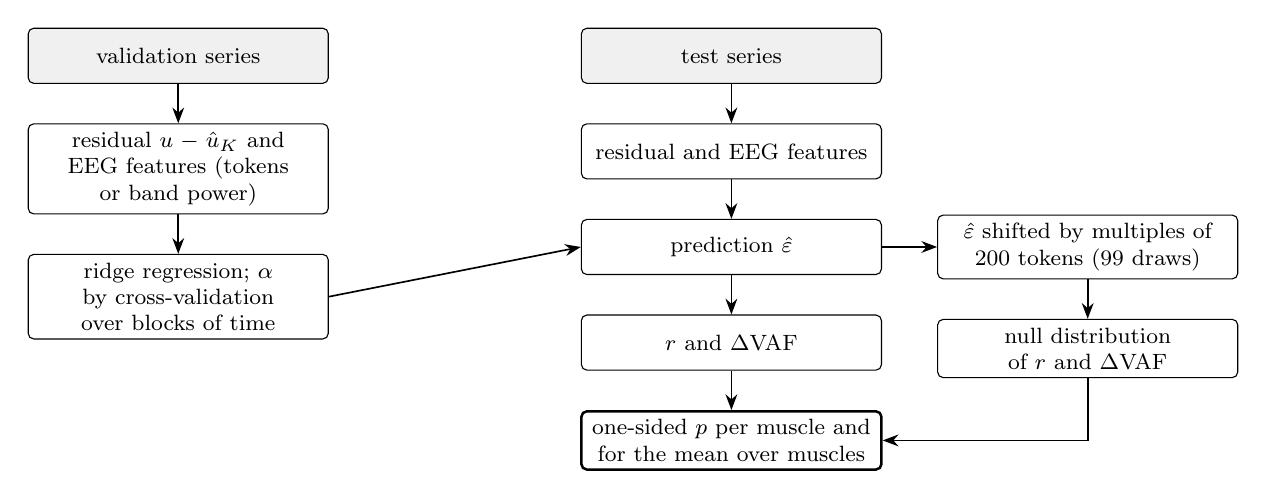
\begin{tikzpicture}[node distance=5mm and 7mm, font=\footnotesize, box/.append style={text width=3.6cm}]
\node[io] (val) {validation series};
\node[box, below=of val] (rv) {residual $u-\hat u_K$ and EEG features (tokens or band power)};
\node[box, below=of rv] (fit) {ridge regression; $\alpha$ by cross-validation over blocks of time};
\node[io, right=32mm of val] (te) {test series};
\node[box, below=of te] (rt) {residual and EEG features};
\node[box, below=of rt] (pr) {prediction $\hat\varepsilon$};
\node[box, below=of pr] (sc) {$r$ and $\Delta\mathrm{VAF}$};
\node[box, right=of pr] (sh) {$\hat\varepsilon$ shifted by multiples of 200 tokens (99 draws)};
\node[box, below=of sh] (nl) {null distribution of $r$ and $\Delta\mathrm{VAF}$};
\node[result, below=of sc] (p) {one-sided $p$ per muscle and for the mean over muscles};
\draw[arr] (val)--(rv); \draw[arr] (rv)--(fit); \draw[arr] (te)--(rt); \draw[arr] (rt)--(pr);
\draw[arr] (fit.east)--(pr.west); \draw[arr] (pr)--(sc); \draw[arr] (pr)--(sh); \draw[arr] (sh)--(nl);
\draw[arr] (sc)--(p); \draw[arr] (nl)|-(p);
\end{tikzpicture}
\end{latin}

\caption{\lr{residual test}.}
\label{fig:residual}
\end{figure}

\subsection{یک دام: موقعیت درون پنجره}

\lr{encoder}های زمانی به هر \lr{token} \lr{sinusoidal positional encoding} اضافه می‌کنند. پس \lr{tokens} \lr{EEG} می‌دانند در کجای پنجره‌ی ۸ ثانیه‌ای هستند. از طرف دیگر، پیش‌بینی پیوسته‌ی \lr{K} از پنجره‌هایی ساخته شده که هر ۴ ثانیه یک بار شروع می‌شوند، پس ممکن است خطای کوچکی با همین دوره‌ی ۴ ثانیه‌ای داشته باشد.

یک \lr{ridge} روی \lr{tokens} می‌تواند این دو الگوی دوره‌ای را به هم ربط دهد، بی آنکه \lr{EEG} واقعاً اطلاعاتی داشته باشد. این اتفاق در آزمون روی داده‌ی کاملاً تصادفی دیده شد: با جابه‌جایی‌های دلخواه، $r$ حدود \lr{۰٫۱} و «معنادار» شد.

راه حل: اگر جابه‌جایی همیشه مضربی از ۴ ثانیه باشد، این الگوی دوره‌ای در داده‌ی جابه‌جاشده هم سر جایش می‌ماند. پس این اثر در \lr{null distribution} هم هست و فقط اطلاعاتی شمرده می‌شود که به زمان واقعی بسته است. ویژگی‌های \lr{band power} اصلاً اطلاعات موقعیت ندارند و از این نظر بررسی تمیزتری هستند.

\subsection{نتایج}

\begin{table}[htbp]
\centering
\small
\caption{\lr{residual test}، ردیف میانگین روی پنج عضله برای هر شرکت‌کننده. \lr{r}: همبستگی باقی‌مانده‌ی پیش‌بینی‌شده و واقعی روی سری‌های آزمون؛ \lr{p}: در برابر همان پیش‌بینی با جابه‌جایی زمانی؛ $\Delta$\lr{VAF}: بهره‌ی \lr{K} به‌علاوه‌ی باقی‌مانده‌ی پیش‌بینی‌شده نسبت به \lr{K} (واحد درصد)؛ ستون آخر همبستگی اصلاحِ خودِ مدل ($F_{eeg}$) با باقی‌مانده.}
\label{tab:res-subj}
\begin{tabular}{lccccccc}
\toprule
شرکت‌کننده & \lr{r} \lr{tokens} & \lr{p} & $\Delta$\lr{VAF} & \lr{r} \lr{band power} & \lr{p} & $\Delta$\lr{VAF} & \lr{r} اصلاح مدل \\
\midrule
\lr{P1} & \lr{۰٫۰۵۵} & \lr{۰٫۰۱} & \lr{−۰٫۰۳} & \lr{۰٫۰۴۱} & \lr{۰٫۰۳} & \lr{−۰٫۰۶} & \lr{۰٫۰۹۲} \\
\lr{P2} & \lr{۰٫۰۸۵} & \lr{۰٫۰۱} & \lr{+۰٫۰۳} & \lr{۰٫۰۸۳} & \lr{۰٫۰۱} & \lr{−۰٫۰۰} & \lr{۰٫۰۰۴} \\
\lr{P3} & \lr{۰٫۱۴۱} & \lr{۰٫۰۱} & \lr{+۰٫۲۴} & \lr{۰٫۱۰۴} & \lr{۰٫۰۱} & \lr{−۰٫۴۸} & \lr{۰٫۰۸۴} \\
\lr{P4} & \lr{۰٫۰۸۸} & \lr{۰٫۰۱} & \lr{+۰٫۰۶} & \lr{۰٫۰۰۶} & \lr{۰٫۳۶} & \lr{−۰٫۱۹} & \lr{۰٫۰۶۴} \\
\lr{P5} & \lr{۰٫۰۶۵} & \lr{۰٫۰۱} & \lr{+۰٫۱۹} & \lr{۰٫۰۳۰} & \lr{۰٫۲۴} & \lr{−۰٫۲۳} & \lr{۰٫۰۸۸} \\
\lr{P6} & \lr{۰٫۰۵۹} & \lr{۰٫۰۱} & \lr{−۰٫۹۷} & \lr{۰٫۰۶۲} & \lr{۰٫۰۳} & \lr{−۰٫۶۳} & \lr{۰٫۱۲۲} \\
\lr{P7} & \lr{۰٫۰۰۱} & \lr{۰٫۶۰} & \lr{−۰٫۰۸} & \lr{−۰٫۰۴۶} & \lr{۱٫۰۰} & \lr{−۰٫۰۸} & \lr{۰٫۱۲۲} \\
\lr{P8} & \lr{۰٫۲۲۶} & \lr{۰٫۰۱} & \lr{+۲٫۳۷} & \lr{۰٫۱۲۲} & \lr{۰٫۰۱} & \lr{+۰٫۴۷} & \lr{۰٫۱۵۲} \\
\lr{P9} & \lr{۰٫۰۷۸} & \lr{۰٫۰۱} & \lr{+۰٫۱۶} & \lr{۰٫۰۴۲} & \lr{۰٫۰۱} & \lr{+۰٫۲۳} & \lr{۰٫۱۴۷} \\
\lr{P10} & \lr{−۰٫۰۵۵} & \lr{۱٫۰۰} & \lr{−۰٫۸۶} & \lr{−۰٫۰۱۲} & \lr{۰٫۸۱} & \lr{−۰٫۵۹} & \lr{−۰٫۰۰۱} \\
\lr{P11} & \lr{۰٫۰۳۹} & \lr{۰٫۰۱} & \lr{−۰٫۱۰} & \lr{۰٫۰۱۷} & \lr{۰٫۱۸} & \lr{+۰٫۰۳} & \lr{−۰٫۰۰۴} \\
\lr{P12} & \lr{۰٫۱۰۱} & \lr{۰٫۰۱} & \lr{+۰٫۱۵} & \lr{۰٫۰۳۶} & \lr{۰٫۰۸} & \lr{−۰٫۰۴} & \lr{۰٫۰۳۷} \\
\midrule
\textbf{میانگین} & \lr{۰٫۰۷۳} &  & \lr{+۰٫۱۰} & \lr{۰٫۰۴۰} &  & \lr{−۰٫۱۳} & \lr{۰٫۰۷۶} \\
\bottomrule
\end{tabular}
\end{table}

\begin{table}[htbp]
\centering
\small
\caption{\lr{residual test} برای هر عضله، میانگین روی ۱۲ شرکت‌کننده؛ ستون‌های تعداد از ۱۲ شمرده شده‌اند.}
\label{tab:res-musc}
\begin{tabular}{ccccccc}
\toprule
عضله & \lr{r} \lr{tokens} & تعداد \lr{p}$\le$۰٫۰۵ & $\Delta$\lr{VAF} & \lr{r} \lr{band power} & تعداد \lr{p}$\le$۰٫۰۵ & $\Delta$\lr{VAF} \\
\midrule
\lr{AD} & \lr{۰٫۰۵۶} & \lr{۷} & \lr{+۰٫۰۴} & \lr{۰٫۰۳۵} & \lr{۴} & \lr{+۰٫۰۲} \\
\lr{BR} & \lr{۰٫۰۷۹} & \lr{۷} & \lr{+۰٫۱۶} & \lr{۰٫۰۲۱} & \lr{۶} & \lr{−۰٫۱۳} \\
\lr{FD} & \lr{۰٫۱۱۸} & \lr{۸} & \lr{+۰٫۱۴} & \lr{۰٫۰۵۲} & \lr{۷} & \lr{−۰٫۴۶} \\
\lr{ED} & \lr{۰٫۰۷۸} & \lr{۷} & \lr{+۰٫۰۸} & \lr{۰٫۰۵۱} & \lr{۴} & \lr{−۰٫۰۳} \\
\lr{FDI} & \lr{۰٫۰۳۶} & \lr{۵} & \lr{+۰٫۰۷} & \lr{۰٫۰۴۲} & \lr{۴} & \lr{−۰٫۰۵} \\
\bottomrule
\end{tabular}
\end{table}


\paragraph{اثر واقعی است.} با \lr{tokens} میانگین $r$ \lr{۰٫۰۷۳} است، در حالی که در \lr{null distribution} \lr{−۰٫۰۰۱} است. در ۱۰ شرکت‌کننده از ۱۲ نفر $p\le0.05$ است؛ از شانس کمتر از یک مورد انتظار می‌رود. با \lr{band power} میانگین $r$ \lr{۰٫۰۴۰} است و در ۶ نفر معنادار.

\paragraph{اما اثر بسیار کوچک است.} $r=0.07$ یعنی حدود \lr{۰٫۵} درصد از واریانس باقی‌مانده. اضافه کردن این پیش‌بینی به \lr{K}، \lr{VAF} را به‌طور میانگین \lr{۰٫۱۰} واحد (با \lr{tokens}) بهتر و \lr{۰٫۱۳} واحد (با \lr{band power}) بدتر می‌کند. فقط در ۷ نفر (\lr{tokens}) و ۲ نفر (\lr{band power}) بهره‌ی \lr{VAF} هم مثبت و هم معنادار است.

\paragraph{استثنا: \lr{P8}.} با \lr{tokens} \lr{VAF} \lr{۲٫۴} واحد بهتر می‌شود و $r$ برای \lr{BR}، \lr{FD} و \lr{ED} تا \lr{۰٫۲۹} می‌رسد. \lr{P8} ضعیف‌ترین \lr{K} را دارد (\lr{VAF} ۵۸ درصد)، پس خطای بیشتری برای توضیح دادن باقی مانده است.

\paragraph{\lr{fusion} همان چیزی را یاد گرفته که هست.} $r_{model}$، یعنی همبستگی اصلاح خود مدل با باقی‌مانده، به‌طور میانگین \lr{۰٫۰۷۶} است؛ هم‌اندازه‌ی \lr{ridge}. پس \lr{fusion} جهت درست را پیدا کرده است. ولی چون اطلاعات این‌قدر کم است، آموزش \lr{gate} را نزدیک صفر نگه داشته است.

\subsection{بحث}

\lr{EEG} در این داده سیگنالی کوچک اما پایدار درباره‌ی آنچه سینماتیک توضیح نمی‌دهد دارد. ارزش پیش‌بینی این سیگنال کمتر از نیم واحد \lr{VAF} است. پس $F\approx K$ نتیجه‌ی درست این داده است، نه نقص \lr{fusion}.

آیا آموزش جداگانه‌ی \lr{fusion} کمکی می‌کرد؟ مثلاً یک مرحله‌ی اضافه فقط برای \lr{fusion}، با هر دو جریان \lr{freeze}‌شده و انتخاب بهترین دوره بر اساس خطای \lr{F}. بر اساس اعداد بالا، در بهترین حالت حدود \lr{۰٫۱} واحد به میانگین و حدود ۲ واحد به \lr{P8} اضافه می‌شد. این بهره هزینه‌ی آموزش دوباره‌ی ۱۲ نفر را توجیه نمی‌کند.

\paragraph{یک احتیاط.} \lr{tokens} بهتر از \lr{band power} عمل کردند. اما \lr{tokens} برای پیش‌بینی \lr{EMG} آموزش دیده‌اند، پس می‌دانند حرکت در چه مرحله‌ای است. ممکن است بخشی از این سیگنال کوچک، زمان‌بندی حرکت یا \lr{artifact} حرکت در \lr{EEG} باشد و نه فرمان قشر حرکتی. پس $r$ معنادار در اینجا \emph{ثابت نمی‌کند} که \lr{EEG} اطلاعات عصبی فراتر از سینماتیک دارد. آزمون بعدی می‌تواند همین \lr{ridge} روی باندها یا الکترودهایی باشد که کمتر در معرض \lr{artifact} حرکت‌اند.

\section{جمع‌بندی و محدودیت‌ها}

\paragraph{آنچه به دست آمد.} \lr{v2} سه پرسش را که مدل پایه در یک خروجی با هم مخلوط می‌کرد جدا کرد.
\begin{enumerate}
\item \textbf{دقت از سینماتیک:} \lr{K} با \lr{VAF} برابر \lr{۷۵٫۸} درصد و \lr{r} برابر \lr{۰٫۸۷۲} در هر ۱۲ شرکت‌کننده از مدل پایه بهتر است و دامنه را در هر سه وزن جسم با خطای کمتر از یک درصد پیش‌بینی می‌کند. بافت ۸ ثانیه‌ای، تاریخچه‌ی بلندکردن‌ها، حوزه‌ی جذر و جزء سطح نگه‌داشتن در هزینه پشت این بهبودند.
\item \textbf{\lr{EEG} به‌تنهایی:} \lr{E} با \lr{r} برابر \lr{۰٫۶۴۵} در هر ۱۲ نفر از \lr{null test} گذشت؛ \lr{EEG} حالت حرکت را رمز می‌کند.
\item \textbf{\lr{EEG} فراتر از سینماتیک:} \lr{F} برابر \lr{K} است. \lr{residual test} سیگنالی واقعی اما بسیار کوچک یافت (\lr{r} حدود \lr{۰٫۰۷}، کمتر از نیم واحد \lr{VAF}) که ماژول \lr{fusion} هم همان را یافته بود.
\end{enumerate}

\paragraph{تفسیرپذیری.} قاعده‌ی «یک مخلوط‌کننده» و \lr{recorder} بیرونی، \lr{rollout}، جریان، \lr{gradient-weighted rollout} و نمای هر لایه را برای هر خروجی و در همه‌ی لایه‌ها بدون حالت خاص ممکن کرد. سنجش نقشه‌ها نشان داد \lr{gradient-weighted rollout} قابل‌اعتمادترین روش است (بهترین در \lr{deletion check}، کمترین شباهت با مدل به‌هم‌ریخته). \lr{attention flow} در این معماری اشباع می‌شود و فقط در برابر خط پایه‌ی توجه یکنواخت معنا دارد. نقشه‌های الکترود \lr{E} کانونی بالای قشر حرکتی چپ دارند، اما سهم الکترودهای پیشانی و پس‌سری هشدار می‌دهد که بخشی از اطلاعات ممکن است \lr{artifact} باشد.

\paragraph{محدودیت‌ها.}
\begin{itemize}
\item \lr{rollout} و جریان فقط وزن‌های توجه را می‌بینند؛ وزن \lr{۰٫۵} \lr{residual connection} یک قرارداد است. روش‌های گرادیانی موضعی و مرتبه‌ی اول‌اند.
\item \lr{plain rollout} \lr{K} در \lr{weight-shuffle check} شباهت بالایی دارد (\lr{۰٫۴۷})؛ شکل آن بیشتر از ساختار مدل می‌آید تا از یادگیری.
\item پنجره‌های رخدادهای نزدیک هم‌پوشانی دارند، پس $p$ مقایسه‌ی رخداد با استراحت تقریبی است.
\item همه‌ی نتایج برای هر شرکت‌کننده جداگانه است؛ تعمیم به شرکت‌کننده‌ی تازه آزموده نشده است.
\item پیش‌بینی برون‌خط است: هر \lr{token} از کل پنجره‌ی ۸ ثانیه‌ای، از جمله آینده، استفاده می‌کند.
\item سقف داده (به‌ویژه برای \lr{FD}) هر بهبود دیگری را محدود می‌کند.
\end{itemize}

\paragraph{بازتولید.} کد در شاخه‌ی \lr{KG-GT-v2} (بسته‌ی \lr{v2/} و دفترچه‌ی \lr{main\_v2.ipynb}) است. جدول‌ها و شکل‌های این گزارش را اسکریپت \lr{v2-report/build\_assets.py} از نتایج ذخیره‌شده می‌سازد و هیچ مدلی را اجرا نمی‌کند.

\begin{thebibliography}{99}
\bibitem{luciw2014} \lr{M. D. Luciw, E. Jarocka, B. B. Edin. Multi-channel EEG recordings during 3,936 grasp and lift trials with varying weight and friction. Scientific Data, 1:140047, 2014.}
\bibitem{vaswani2017} \lr{A. Vaswani et al. Attention is all you need. NeurIPS, 2017.}
\bibitem{velickovic2018} \lr{P. Veli\v{c}kovi\'c et al. Graph attention networks. ICLR, 2018.}
\bibitem{abnar2020} \lr{S. Abnar, W. Zuidema. Quantifying attention flow in transformers. ACL, 2020.}
\bibitem{chefer2021} \lr{H. Chefer, S. Gur, L. Wolf. Generic attention-model explainability for interpreting bi-modal and encoder-decoder transformers. ICCV, 2021.}
\bibitem{shrikumar2016} \lr{A. Shrikumar, P. Greenside, A. Shcherbina, A. Kundaje. Not just a black box: learning important features through propagating activation differences. arXiv:1605.01713, 2016.}
\bibitem{samek2017} \lr{W. Samek, A. Binder, G. Montavon, S. Lapuschkin, K.-R. M\"uller. Evaluating the visualization of what a deep neural network has learned. IEEE TNNLS, 28(11), 2017.}
\bibitem{adebayo2018} \lr{J. Adebayo, J. Gilmer, M. Muelly, I. Goodfellow, M. Hardt, B. Kim. Sanity checks for saliency maps. NeurIPS, 2018.}
\bibitem{nichols2002} \lr{T. E. Nichols, A. P. Holmes. Nonparametric permutation tests for functional neuroimaging: a primer with examples. Human Brain Mapping, 15(1), 2002.}
\bibitem{lin1989} \lr{L. I. Lin. A concordance correlation coefficient to evaluate reproducibility. Biometrics, 45(1), 1989.}
\end{thebibliography}


\end{document}
